\documentclass[11pt,a4paper]{report}
\usepackage{fontspec}
\setmainfont{Latin Modern Roman}
\setsansfont{Latin Modern Sans}
% Characters missing in Latin Modern Mono (the emoji and Chinese characters in
% examples/01_hello.s) are taken from macOS fonts, if they exist.
\directlua{luaotfload.add_fallback("monofallback",
  {"Arial Unicode MS:mode=harf;", "Apple Color Emoji:mode=harf;"})}
\setmonofont{Latin Modern Mono}[Scale=0.88,RawFeature={fallback=monofallback}]
\usepackage[margin=27mm]{geometry}
\usepackage[skip=\medskipamount,indent=0pt]{parskip}
\usepackage{amsmath,amssymb}
\usepackage{microtype}
\usepackage{xcolor}
\usepackage{graphicx}
\usepackage{listings}
\usepackage{fancyvrb}
\usepackage{etoolbox}
\usepackage{booktabs}
\usepackage{array}
\usepackage{longtable}
\usepackage{enumitem}
\usepackage[font=small,labelfont=bf]{caption}
\usepackage{tikz}
\usepackage[most]{tcolorbox}
\usetikzlibrary{arrows.meta,positioning,fit,calc,decorations.pathreplacing,patterns,
  circuits.logic.US,matrix}
\usepackage{xurl}
\usepackage{titlesec}
\titleformat{\chapter}[display]{\normalfont\bfseries}{\large\chaptertitlename\ \thechapter}{4pt}{\LARGE}
\titlespacing*{\chapter}{0pt}{0pt}{16pt}
\usepackage{hyperref}
\hypersetup{
  colorlinks=true,
  linkcolor=blue!50!black,
  urlcolor=blue!50!black,
  linktoc=all,
  bookmarksnumbered=true,
  bookmarksopen=true,
  bookmarksopenlevel=0,
  pdftitle={ULM on ICE: Building a Computer on an FPGA, Step by Step},
  pdfauthor={Michael C. Lehn}
}

% Start a section on the next page if it would get only a line or two here.
\usepackage{needspace}
\usepackage{placeins}
\let\plainsection\section
\renewcommand{\section}{\needspace{6.5\baselineskip}\plainsection}

\definecolor{codebg}{RGB}{247,248,250}
\definecolor{codekw}{RGB}{0,70,140}
\definecolor{codecomment}{RGB}{95,105,115}
\definecolor{termbg}{RGB}{240,242,238}
\lstdefinestyle{code}{
  basicstyle=\ttfamily\small,
  keywordstyle=\color{codekw},
  commentstyle=\color{codecomment},
  backgroundcolor=\color{codebg},
  frame=single,
  rulecolor=\color{black!15},
  columns=fullflexible,
  keepspaces=true,
  showstringspaces=false,
  breaklines=true,
  tabsize=8,
  aboveskip=6pt,
  belowskip=6pt
}
\lstdefinelanguage{SystemVerilog}[]{Verilog}{
  morekeywords={logic,always_comb,always_ff,always_latch,typedef,enum,struct,
    packed,interface,endinterface,modport,package,endpackage,import,unique,
    priority,int,bit,byte,shortint,longint,localparam,genvar,generate,
    endgenerate},
  sensitive=true
}
% Commands typed at a prompt and what they print.
\lstdefinestyle{term}{
  style=code,
  language={},
  basicstyle=\ttfamily\footnotesize,
  backgroundcolor=\color{termbg},
  breaklines=true,
  breakindent=2em,
  postbreak={}
}
% \endgraf drops the indentation of an enclosing list, so we restore it by hand.
\makeatletter
\lstnewenvironment{terminal}{\endgraf\noindent\hskip\@totalleftmargin\minipage{\linewidth}\lstset{style=term}}{\endminipage\endgraf}
\makeatother
\lstset{style=code,language=SystemVerilog}

% Files of the repository, given relative to its top directory.  Whole files
% may break across pages; \svpart keeps a part of a file on one page.
\newcommand{\svfile}[2][]{\lstinputlisting[language=SystemVerilog,title={\texttt{\detokenize{#2}}},#1]{../#2}}
\newcommand{\svpart}[2]{\par\noindent\begin{minipage}{\linewidth}\lstinputlisting[language=SystemVerilog,title={\texttt{\detokenize{#2}}},#1]{../#2}\end{minipage}\par}
\newcommand{\cppfile}[2][]{\lstinputlisting[language=C++,title={\texttt{\detokenize{#2}}},#1]{../#2}}
\newcommand{\cpppart}[2]{\par\noindent\begin{minipage}{\linewidth}\lstinputlisting[language=C++,title={\texttt{\detokenize{#2}}},#1]{../#2}\end{minipage}\par}
\newcommand{\makefilepart}[2]{\par\noindent\begin{minipage}{\linewidth}\lstinputlisting[language=make,title={\texttt{\detokenize{#2}}},#1]{../#2}\end{minipage}\par}
% A file shown verbatim, for files with characters outside of Latin-1, which
% listings would put in the wrong order (examples/01_hello.s).
\newcommand{\verbfile}[1]{\par\noindent\begin{tcolorbox}[colback=codebg,colframe=black!15,
  boxrule=0.4pt,sharp corners,left=3pt,right=3pt,top=2pt,bottom=2pt,
  title={\texttt{\detokenize{#1}}},coltitle=black,colbacktitle=white,
  fonttitle=\small,toptitle=0pt,bottomtitle=2pt,halign title=center]
  \VerbatimInput[fontsize=\small,tabsize=8]{../#1}\end{tcolorbox}\par}
% Output of the tools, captured in the directory output.
\newcommand{\outputfile}[1]{\par\noindent\begin{minipage}{\linewidth}\lstinputlisting[style=term,basicstyle=\ttfamily\scriptsize]{output/#1}\end{minipage}\par}

\setlist[description]{leftmargin=1.5em,itemsep=2pt,topsep=2pt,font=\normalfont\bfseries}
\setlist[itemize]{itemsep=2pt,topsep=2pt}
\setlist[enumerate]{itemsep=4pt,topsep=2pt}
\setlength{\emergencystretch}{1.5em}

% Something for the reader to do.
\definecolor{tryitbar}{RGB}{40,90,190}
\newcounter{exercise}[chapter]
\renewcommand{\theexercise}{\thechapter.\arabic{exercise}}
\newenvironment{exercise}
  {\par\medskip\refstepcounter{exercise}\noindent
   \begin{list}{}{\leftmargin=9pt\rightmargin=0pt\topsep=0pt}\item\relax
   \textcolor{tryitbar}{\textbf{Exercise~\theexercise.}}\ }
  {\end{list}\medskip}

% Solutions at the end of a chapter, in the order of the exercises.
\newcounter{solution}[chapter]
\newcommand{\solutions}{\clearpage\section{Solutions}\setcounter{solution}{0}}
\newcommand{\solution}{\par\medskip\refstepcounter{solution}\noindent
  \textcolor{tryitbar}{\textbf{Exercise~\thechapter.\arabic{solution}.}}\ }

% A pitfall.
\definecolor{warnbar}{RGB}{170,70,20}
\newenvironment{pitfall}
  {\par\medskip\noindent
   \begin{list}{}{\leftmargin=9pt\rightmargin=0pt\topsep=0pt}\item\relax
   \textcolor{warnbar}{\textbf{Pitfall.}}\ }
  {\end{list}\medskip}

% Exclusive or: a dotted \lor.
\newcommand{\xor}{\mathbin{\dot{\lor}}}

% Terms defined in the text.
\newcommand{\term}[1]{\emph{#1}}
% Inline code on a light gray background, as on GitHub.
\definecolor{inlinebg}{RGB}{236,238,241}
\tcbset{inlinecode/.style={on line,colback=inlinebg,colframe=inlinebg,frame empty,boxrule=0pt,
  arc=2pt,boxsep=0pt,left=2pt,right=2pt,top=1pt,bottom=1pt,before upper={\vphantom{(}}}}
% \smash: the background may reach into the line spacing, but never changes it.
\DeclareRobustCommand{\cc}[1]{\smash{\tcbox[inlinecode]{\ttfamily\detokenize{#1}}}}

% Figures.
\tikzset{
  box/.style={draw,rounded corners=2pt,align=center,font=\small},
  toolbox/.style={box,fill=blue!7,minimum height=9mm},
  filebox/.style={box,fill=black!5,minimum height=9mm},
  chipbox/.style={box,fill=green!10},
  arrow/.style={->,>=Stealth,thick,draw=black!65},
  biarrow/.style={<->,>=Stealth,thick,draw=black!65},
  note/.style={font=\footnotesize,align=center,text=black!70},
  wire/.style={thick,draw=black!80},
  % timing diagrams: \draw[signal] ... with high at y=0.5, low at y=0
  signal/.style={thick,draw=blue!60!black},
  clocksig/.style={thick,draw=black!70},
}


\title{ULM on ICE\\[6pt]
       \large Building a Computer on an FPGA, Step by Step}
\author{Michael C. Lehn}
\date{}

\begin{document}
\maketitle
\tableofcontents

\chapter*{Preface}
\addcontentsline{toc}{chapter}{Preface}

The ULM, the \emph{Ulm Lecture Machine}, is the computer we use in our lectures
to explain what a machine does with a program. It has sixteen 64-bit registers,
a memory, instructions of 32 bits, and a few instructions to read and write
characters. Until now it existed as a simulator. In these notes we build it as
real hardware: on an FPGA, a chip whose circuits are not fixed when it leaves
the factory but are configured later.

We do not build it in one go. The repository \cc{ulm-on-ice} consists of nine
directories, \cc{01_logic_gates} to \cc{09_ulm_on_ice}, and each of them is a
small, complete project that you can simulate, put on the FPGA and try out.
The first one connects two buttons to two LEDs through a few logic gates, the
last one is the ULM, running programs that we type in through a terminal. Each
step adds one new idea, and each chapter of these notes is one step.

On the way you should learn three things:
\begin{itemize}
\item what an FPGA is, and what it can and cannot do;
\item how we describe a circuit in SystemVerilog, and how the tools turn this
  description into a configuration of the FPGA;
\item how a computer is built from parts that you know: gates, flip-flops,
  multiplexers, adders, registers and memory.
\end{itemize}

We assume that you know logic gates and flip-flops, and that you have built
small circuits with a tool like CircuitVerse: an adder, a multiplexer, a
register. This is all the hardware background we need. The rest is introduced
when a step needs it, and only as much as that step needs.

Most of all, we treat SystemVerilog as what it is: \emph{a textual
representation of circuits}. It looks like a programming language, and this is
the source of most misunderstandings. A line of SystemVerilog does not do
something at some point in time. It says how wires are connected. Whenever a
construct is new, we first ask which circuit it describes.

The notes are a tutorial, so they are meant to be worked through with the
repository and the board at hand. Every listing of SystemVerilog is taken
directly from the repository, and all the output shown was produced by the
tools on a Mac (yosys 0.70, nextpnr 0.11.1, Verilator 5.052, sv2v 0.0.13). Your
output may differ in details.

The board is an \href{https://1bitsquared.com/products/icebreaker}{iCEBreaker},
with the small button-and-LED module that comes with it and the 7-segment
display module from the same manufacturer. The idea for the material grew out
of the course \emph{HPC0}, where we build a Mini-ALU in CircuitVerse, first
look at its description in SystemVerilog, and then put it on exactly this
board.

\part{Getting Started}
\label{part:start}

\chapter{The Big Picture}
\label{ch:overview}

Before we describe a single circuit, we need a mental model of the chip that
will contain it. This chapter answers three questions: what is inside an FPGA,
what is on our board, and which tools bring a description in SystemVerilog onto
the chip.

\section{What an FPGA Is}
\label{sec:fpga}

A processor, say the CPU of your laptop, is a fixed circuit. It was designed
once, and all chips of this type contain the same gates connected by the same
wires. What changes is the program it runs.

An FPGA, a \term{field programmable gate array}, is different. It is a chip
that consists of a large number of small, identical building blocks and of
wires between them, and both are \emph{configurable}: which Boolean function a
block computes, and which blocks are connected to which. The configuration is
loaded into the chip when it is switched on. So the circuit itself is what we
change, not a program running on it. If we configure an FPGA as a processor,
then this processor can in turn run programs, and that is exactly what we do
in the last step.

The building blocks of our FPGA, a Lattice iCE40UP5K, come in a few kinds:
\begin{description}
\item[Logic cells.] The workhorse. A logic cell consists of a lookup table with
  four inputs, a flip-flop, and a little extra logic for adding numbers. The
  iCE40UP5K has 5280 of them.
\item[Routing.] Wires between the logic cells, with switches that decide which
  wires are connected. Most of the area of an FPGA is routing, not logic.
\item[I/O pins.] The connections to the outside world, here buttons, LEDs, the
  display and the USB chip on the board.
\item[Memory blocks.] Ready-made memory, because building memory from
  flip-flops would use up the logic cells quickly. We meet them in
  Chapter~\ref{ch:step07}.
\end{description}
The lookup table is the part that needs explaining, and it is simpler than its
name suggests.

\section{A Lookup Table Is a Multiplexer}
\label{sec:lut}

You know the multiplexer from CircuitVerse: it has data inputs, control inputs,
and one output, and the control bits select which data input appears at the
output. A multiplexer with four control bits selects one of $2^4 = 16$ data
inputs.

Now take such a 16-to-1 multiplexer and do not connect its data inputs to
signals. Instead, fix each of them to a constant 0 or 1 when the chip is
configured. These 16 constants are the \term{configuration bits} of the
lookup table, and the four control inputs are its actual inputs
(Figure~\ref{fig:lut}). This is a \term{lookup table}, or \term{LUT} for short.

\begin{figure}[ht]
\centering
\begin{tikzpicture}[x=1mm,y=1mm]
  % the multiplexer
  \draw[thick,fill=green!8] (0,0) -- (0,64) -- (18,54) -- (18,10) -- cycle;
  \node[font=\small] at (9,32) {MUX};
  \foreach \k in {0,...,15} {
    \pgfmathsetmacro{\y}{60-3.7*\k}
    \draw[wire] (-12,\y) -- (0,\y);
    \node[font=\scriptsize,anchor=east] at (-12,\y) {$t_{\k}$};
  }
  \node[note,anchor=east] at (-20,32) {16 configuration\\bits, set when\\the FPGA is\\configured};
  \draw[decorate,decoration={brace,amplitude=4pt},thick,black!60]
    (-19,2) -- (-19,62);
  \foreach \j/\name in {0/x_0,1/x_1,2/x_2,3/x_3} {
    \pgfmathsetmacro{\x}{3+4*\j}
    \draw[wire] (\x,-8) -- (\x,{\x*10/18});
    \node[font=\scriptsize,anchor=north] at (\x,-8) {$\name$};
  }
  \node[note,anchor=north] at (9,-13) {inputs of the LUT\\(control bits of the multiplexer)};
  \draw[wire] (18,32) -- (32,32) node[right,font=\small] {$f(x_3,x_2,x_1,x_0) = t_{8x_3+4x_2+2x_1+x_0}$};
\end{tikzpicture}
\caption{A lookup table with four inputs: a 16-to-1 multiplexer whose data
inputs are constants. The inputs of the LUT select one of them.}
\label{fig:lut}
\end{figure}

What does such a LUT compute? The four input bits, read as a binary number
$i = 8x_3 + 4x_2 + 2x_1 + x_0 \in \{0, \dots, 15\}$, select the configuration
bit $t_i$. So the LUT computes the Boolean function
\[
  f\colon \{0,1\}^4 \to \{0,1\}, \qquad
  f(x_3, x_2, x_1, x_0) = t_{8x_3+4x_2+2x_1+x_0},
\]
and the 16 configuration bits are nothing but the last column of its truth
table. Every Boolean function of four variables has a truth table with 16 rows,
so a LUT can compute \emph{every} such function: there are $2^{16} = 65536$ of
them, one for each way to choose the configuration bits.

This is the whole trick of an FPGA. There are no AND or OR gates on the chip
waiting to be connected. A circuit that you draw with gates is translated into
Boolean functions of at most four inputs each, and every one of these functions
becomes a LUT with the right 16 bits. A function of more than four inputs is
split into several LUTs, the output of one feeding an input of the next.

\begin{exercise}
Which configuration bits $t_0, \dots, t_{15}$ make a LUT compute the
function $f(x_3,x_2,x_1,x_0) = x_3 \wedge x_2$? Which ones make it compute
$x_0 \xor x_1 \xor x_2 \xor x_3$?
\end{exercise}

\section{Flip-Flops, and Why the Clock Matters}
\label{sec:ff-intro}

A circuit of LUTs alone is combinational: its outputs depend only on its
current inputs. To store something we need flip-flops, and every logic cell has
one right behind its LUT. The output of the LUT can go out of the logic cell
directly, or into the flip-flop, which takes it over at the rising edge of a
clock.

On our board a crystal oscillator delivers a clock of 12\,MHz, that is
$12 \cdot 10^6$ rising edges per second, one every $83.3$\,ns. All flip-flops
in our designs use this one clock (or are meant to, see
Section~\ref{sec:step02-pins}). Between two edges, the signals have to travel
from the flip-flops through LUTs and wires to the next flip-flops and settle
there. This takes time, and so the tools tell us after placing the design how
fast the clock could be. For our larger designs this will be a real
limitation.

\section{The Board}
\label{sec:board}

The iCEBreaker (Figure~\ref{fig:board}) carries the FPGA, the 12\,MHz
oscillator, a flash memory that stores the configuration, and a USB chip. The
USB chip has two jobs: it writes the configuration into the flash, and it
provides a serial line between your computer and the FPGA, which we use from
Chapter~\ref{ch:step06} on.

\begin{figure}[ht]
\centering
\begin{tikzpicture}[node distance=6mm and 22mm]
  \node[chipbox,minimum width=34mm,minimum height=24mm] (fpga) {iCE40UP5K\\[-2pt]\footnotesize FPGA};
  \node[box,fill=black!5,left=of fpga,minimum width=24mm,minimum height=10mm,yshift=8mm] (usb) {USB chip\\[-2pt]\footnotesize FTDI FT2232H};
  \node[box,fill=black!5,left=of fpga,minimum width=24mm,minimum height=10mm,yshift=-8mm] (flash) {flash\\[-2pt]\footnotesize 16\,MiB};
  \node[box,fill=black!5,above=of fpga,minimum width=24mm] (osc) {oscillator\\[-2pt]\footnotesize 12\,MHz};
  \node[box,fill=yellow!12,right=12mm of fpga,minimum width=28mm,yshift=10mm] (pmod1) {PMOD 1A\\[-2pt]\footnotesize 7-segment display};
  \node[box,fill=yellow!12,right=12mm of fpga,minimum width=28mm,yshift=-10mm] (pmod2) {PMOD 2\\[-2pt]\footnotesize 3 buttons, 5 LEDs};
  \node[left=10mm of usb,note] (pc) {your\\computer};
  \draw[biarrow] (pc) -- node[above,note]{USB} (usb);
  \draw[arrow] (usb) -- node[left,note]{writes} (flash);
  \draw[arrow] (flash) -- node[above,note]{configuration} (fpga.west |- flash);
  \draw[biarrow] (usb) -- node[above,note]{serial} (fpga.west |- usb);
  \draw[arrow] (osc) -- node[right,note]{clock} (fpga);
  \draw[biarrow] (fpga.east |- pmod1) -- (pmod1);
  \draw[biarrow] (fpga.east |- pmod2) -- (pmod2);
\end{tikzpicture}
\caption{What is on the board, and how the parts are connected.}
\label{fig:board}
\end{figure}

The FPGA forgets its configuration when the power goes off. At power-up it
reads the configuration from the flash, and so the flash is what we program.

On the right edge of the board are connectors in the PMOD format, a simple
standard for small extension modules. On one we plug the module with three
buttons and five LEDs, on another the 7-segment display with two digits.

Which wire of the FPGA leads to which button is not something the FPGA knows.
The file \cc{icebreaker.pcf} at the top of the repository gives the pins of
the chip names that we can use in our designs. A few lines of it:
\begin{terminal}
# 12 MHz clock
set_io -nowarn CLK        35
...
# LEDs and Buttons (PMOD 2)
set_io -nowarn LED1       26
set_io -nowarn LED2       27
...
set_io -nowarn BTN1       20
set_io -nowarn BTN2       19
\end{terminal}
So pin 35 of the chip is called \cc{CLK}, and pin 20 \cc{BTN1}. When a design
has an input called \cc{BTN1}, it is connected to the first button.

\section{From a Description to a Configured Chip}
\label{sec:toolflow}

Between the SystemVerilog file and the configured chip there are four tools,
and it pays to know what each of them does. Each one reads a file and writes
the next (Figure~\ref{fig:toolflow}).

\begin{figure}[ht]
\centering
\begin{tikzpicture}[node distance=5mm and 7mm]
  \node[filebox] (sv) {\cc{test.sv}};
  \node[toolbox,right=of sv] (sv2v) {\textbf{sv2v}\\[-2pt]\footnotesize translate};
  \node[filebox,right=of sv2v] (v) {\cc{test.v}};
  \node[toolbox,right=of v] (yosys) {\textbf{yosys}\\[-2pt]\footnotesize synthesize};
  \node[filebox,right=of yosys] (json) {\cc{test.json}};
  \node[toolbox,below=9mm of json] (pnr) {\textbf{nextpnr}\\[-2pt]\footnotesize place \& route};
  \node[filebox,left=of pnr] (asc) {\cc{test.asc}};
  \node[toolbox,left=of asc] (pack) {\textbf{icepack}\\[-2pt]\footnotesize pack bits};
  \node[filebox,left=of pack] (bin) {\cc{test.bin}};
  \node[toolbox,left=of bin] (prog) {\textbf{iceprog}\\[-2pt]\footnotesize write flash};
  \node[filebox,right=of pnr] (pcf) {\cc{icebreaker.pcf}};
  \draw[arrow] (sv) -- (sv2v); \draw[arrow] (sv2v) -- (v);
  \draw[arrow] (v) -- (yosys); \draw[arrow] (yosys) -- (json);
  \draw[arrow] (json) -- (pnr); \draw[arrow] (pcf) -- (pnr);
  \draw[arrow] (pnr) -- (asc); \draw[arrow] (asc) -- (pack);
  \draw[arrow] (pack) -- (bin); \draw[arrow] (bin) -- (prog);
\end{tikzpicture}
\caption{The tools between a description in SystemVerilog and the
configuration in the flash of the board. \cc{make synth} runs everything up to
\cc{test.bin}, \cc{make prog} also \cc{iceprog}.}
\label{fig:toolflow}
\end{figure}

\begin{description}
\item[sv2v] translates SystemVerilog into plain Verilog. Verilog is the older
  language from which SystemVerilog grew; yosys understands only part of
  SystemVerilog, but all of Verilog. For our first designs the translation
  hardly changes anything; later, SystemVerilog features such as interfaces
  and packages are translated into Verilog that means the same.
\item[yosys] \term{synthesizes} the design: it turns the description into a
  \term{netlist}, a list of the building blocks of our FPGA (LUTs with their 16
  bits, flip-flops, memory blocks) and of the wires between them. It also
  simplifies the logic as far as it can. Nothing is placed on the chip yet.
\item[nextpnr] \term{places} every building block of the netlist on one of the
  physical blocks of the chip and \term{routes} the wires, that is, it chooses
  the switches of the routing so that the right blocks are connected. Here the
  pin names from \cc{icebreaker.pcf} come in. Then it computes how long the
  signals take, and how fast the clock may be.
\item[icepack] converts the result into the bit pattern that the FPGA loads at
  power-up, the \term{bitstream}.
\item[iceprog] writes the bitstream through USB into the flash and restarts
  the FPGA, which then loads it.
\end{description}

We do not call these tools by hand. Every step directory contains the same
\cc{Makefile} (it is a link to the one in \cc{01_logic_gates}), and its
targets do it for us. The design is always in \cc{test.sv}, with the top
module called \cc{test}.

Next to this path to the chip there is a second one that does not need the
board at all: \term{simulation}. The tool Verilator translates the design into
a C++ class, and a small C++ program, the \term{testbench}, sets the inputs of
this class step by step and records how all signals change. We look at these
recordings in a waveform viewer. Chapter~\ref{ch:step01} shows both paths for
our first design. Appendix~\ref{app:tools} lists all \cc{make} targets.

\solutions

\solution
For $x_3 \wedge x_2$, the output is 1 exactly when $8x_3 + 4x_2 + 2x_1 + x_0
\ge 12$, that is, for the indices 12, 13, 14, 15. So $t_{12} = t_{13} = t_{14}
= t_{15} = 1$ and all other bits are 0. Written from $t_{15}$ down to $t_0$, as
yosys does it (Section~\ref{sec:step01-yosys}):
\cc{1111000000000000}.

For $x_0 \xor x_1 \xor x_2 \xor x_3$, the output is 1 exactly when the
index $i$ has an odd number of ones in binary: $i = 1, 2, 4, 7, 8, 11, 13, 14$.
From $t_{15}$ down to $t_0$: \cc{0110100110010110}.

\chapter{Step 01: Logic Gates}
\label{ch:step01}

Our first design has no state at all: two buttons, two LEDs, and a few gates in
between. This is little hardware, but enough to meet the basic parts of
SystemVerilog, to follow the design through all the tools of
Figure~\ref{fig:toolflow}, and to simulate it. Everything is in the directory
\cc{01_logic_gates}.

\section{The Circuit}
\label{sec:step01-circuit}

Call the two buttons $a$ and $b$ (pressed means 1) and the two LEDs
$\mathit{out}_1$ and $\mathit{out}_2$ (1 means on). The circuit computes
\[
  \mathit{out}_1 = (a \wedge b) \vee a, \qquad
  \mathit{out}_2 = a \vee b .
\]
You would draw it in CircuitVerse as in Figure~\ref{fig:step01-netlist}: an AND
gate and two OR gates. In fact, this figure was not drawn by hand: it was
generated from the SystemVerilog description by \cc{make png}, which we come
back to in Section~\ref{sec:step01-pictures}.

\begin{figure}[ht]
\centering
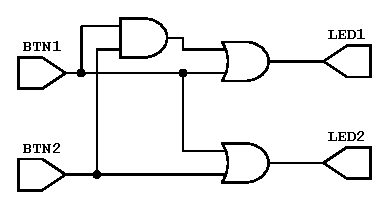
\includegraphics[width=0.62\linewidth]{figures/01_netlist.pdf}
\caption{The circuit of step 01, as drawn by \cc{make svg} from \cc{test.sv}.
The pins on the left and right are the ports of the module.}
\label{fig:step01-netlist}
\end{figure}

\section{The Description in SystemVerilog}
\label{sec:step01-sv}

This is the complete description:

\svfile{01_logic_gates/test.sv}

Read it as a description of the circuit in Figure~\ref{fig:step01-netlist},
piece by piece.

\textbf{A module is a box with pins.} Everything between \cc{module} and
\cc{endmodule} describes one circuit, here called \cc{test}. The list in
parentheses are its \term{ports}: the wires that leave the box, each one an
\cc{input} or an \cc{output}. In CircuitVerse terms, a module is what you get
when you turn a circuit into a subcircuit, and the ports are its inputs and
outputs.

Because \cc{test} is the outermost module, the \term{top module}, its ports
are the pins of the chip. Their names are not arbitrary: \cc{BTN1}, \cc{BTN2},
\cc{LED1} and \cc{LED2} are names from \cc{icebreaker.pcf}
(Section~\ref{sec:board}), and that is how nextpnr knows which pin of the FPGA
each port is.

\textbf{\cc{logic} declares a signal.} The line \cc{logic a, b;} declares two
wires inside the box, each carrying one bit. The type \cc{logic} says only
that the signal carries a logic value; whether it ends up as a plain wire or as
the output of a flip-flop follows from how we use it, as we see in the next
chapter.

\textbf{\cc{assign} connects.} \cc{assign a = BTN1;} says that the wire
\cc{a} is permanently connected to the input \cc{BTN1}. It is not an
assignment in the sense of a programming language, which happens once when the
line is executed. It is a statement about the circuit that holds all the time:
whatever value \cc{BTN1} has, \cc{a} has it too. The four \cc{assign}
statements only give the pins more convenient names. This separates the logic
of our design (\cc{a}, \cc{b}, \cc{out1}, \cc{out2}) from the question which
pin is which, and we can change one without the other.

\textbf{\cc{always_comb} describes combinational logic.} The block
\begin{lstlisting}
always_comb begin
    out1 = a & b | a;
    out2 = a | b;
end
\end{lstlisting}
says: \cc{out1} and \cc{out2} are computed from the signals on the right-hand
sides, by a circuit without memory. Whenever an input changes, the outputs
follow. The operators are the Boolean operations you know:
\begin{center}
\begin{tabular}{cccl}
\toprule
SystemVerilog & logic & name & \\
\midrule
\cc{&} & $\wedge$ & AND & \\
\cc{|} & $\vee$ & OR & \\
\cc{^} & $\xor$ & XOR & (exclusive or) \\
\cc{~} & $\neg$ & NOT & \\
\bottomrule
\end{tabular}
\end{center}
As in arithmetic, where $\cdot$ binds stronger than $+$, \cc{&} binds stronger
than \cc{|}, so \cc{a & b | a} means \cc{(a & b) | a}.

Here the two statements in the block are independent, so their order does not
matter at all. We could also have written \cc{assign out1 = a & b | a;}, which
describes the same circuit. \cc{always_comb} becomes useful when the logic
needs case distinctions, which we see in later steps.

\begin{pitfall}
SystemVerilog looks like a programming language, and the \cc{=} in
\cc{always_comb} looks like an assignment that is executed at some point. It is
not. The whole module describes a circuit that exists all the time, and all of
its parts work in parallel. There is no ``first line'' that runs before the
second, just as there is no first gate in Figure~\ref{fig:step01-netlist}.
\end{pitfall}

\begin{exercise}
\label{ex:step01-absorb}
Simplify $(a \wedge b) \vee a$. What does that mean for \cc{LED1}?
\end{exercise}

\section{From test.sv to the Chip}
\label{sec:step01-synth}

In the directory \cc{01_logic_gates}, the command \cc{make synth} runs the
tools of Figure~\ref{fig:toolflow} up to the bitstream. It prints the
commands it runs:

\outputfile{step01_make_synth.txt}

Before that, \cc{make} has called \cc{sv2v} to produce \cc{test.v}:

\outputfile{step01_make_v.txt}

The option \cc{--define=SYNTHESIS} matters only from step 08 on: there, parts
of a file are meant for simulation only, and \cc{SYNTHESIS} switches them off.

\subsection*{What yosys makes of it}
\label{sec:step01-yosys}

yosys writes its report to \cc{test.log}. The interesting part is at the end, a
list of the building blocks of the netlist:

\outputfile{step01_yosys_stat.txt}

Four ports, six wires, and exactly \emph{one} building block, an
\cc{SB_LUT4}: one lookup table with four inputs. Three gates became a single
LUT, and \cc{LED1} needs no logic at all. If you solved
Exercise~\ref{ex:step01-absorb}, you know why: $(a \wedge b) \vee a = a$, so
\cc{LED1} is simply connected to \cc{BTN1}, and yosys found that out by itself.
\cc{LED2} needs a LUT for $a \vee b$.

Which LUT? The netlist \cc{test.json} contains, for every building block, its
type and its parameters. For our LUT:

\outputfile{step01_lut.txt}

\cc{LUT_INIT} are the 16 configuration bits of Section~\ref{sec:lut}, written
from $t_{15}$ on the left down to $t_0$ on the right. The netlist also says
how the LUT is connected: \cc{BTN1} drives input $x_3$, \cc{BTN2} drives $x_2$,
and the inputs $x_1$ and $x_0$ are fixed to 0. So the LUT selects the bit
\[
  t_{8\cdot\mathtt{BTN1} + 4\cdot\mathtt{BTN2}} ,
\]
which is $t_0 = 0$ if no button is pressed, and $t_4 = t_8 = t_{12} = 1$ if at
least one is. That is $\mathtt{BTN1} \vee \mathtt{BTN2}$, exactly as it should
be. The other twelve bits are never selected; yosys sets them to 1, but any
value would do.

\subsection*{What nextpnr makes of it}

nextpnr places the LUT on one of the 5280 logic cells, connects the four pins,
and reports what it used:

\outputfile{step01_pnr_util.txt}

\cc{ICESTORM_LC} are the logic cells, \cc{SB_IO} the I/O pins. Three logic
cells for one LUT? The other two produce the constants 0 and 1, which the
unused LUT inputs are connected to. (Our report from
Appendix~\ref{app:tools}, \cc{make report}, shows the same numbers.)

nextpnr also computes how long a signal takes from an input pin to an output
pin. For the slowest path, from \cc{BTN2} to \cc{LED2}:

\outputfile{step01_pnr_path.txt}

The numbers in parentheses are positions on the chip: the pin of \cc{BTN2}
at the lower edge, the LUT in the middle, the pin of \cc{LED2} at the upper
edge. The LUT itself takes 1.21\,ns, and the wires to and from it take 9.77\,ns.
This is typical for FPGAs: the routing is usually slower than the logic. For
us it does not matter here, since nobody presses buttons within 11\,ns. Once a
clock is involved, it will.

\subsection*{Programming the board}

\cc{make prog} does everything \cc{make synth} does and then calls
\cc{iceprog test.bin}, which writes the bitstream into the flash of the board
and restarts the FPGA. A second later, the LEDs follow the buttons: \cc{LED1}
is on while the first button is pressed, \cc{LED2} while one of the two is
pressed.

\begin{exercise}
\label{ex:step01-xor}
Replace \cc{out2 = a | b;} by \cc{out2 = a ^ b;}. Predict the value of
\cc{LUT_INIT} for the LUT of \cc{LED2}, then check it with \cc{make test.json}
and a look into \cc{test.json}.
\end{exercise}

\section{Simulation}
\label{sec:step01-sim}

Programming the board is the final test, but it is a poor tool for finding
mistakes: you see only what reaches a pin. In a \term{simulation}, a program
computes how all signals of the design change over time, and we can look at
every one of them.

We use Verilator. It translates the design into a C++ class \cc{Vtest}, whose
member variables are the ports of the module. A small C++ program, the
\term{testbench} \cc{tb_test.cpp}, creates such an object, sets its inputs and
calls \cc{eval()}, which computes the outputs. Here is its main loop:

\cpppart{firstline=21,lastline=45}{01_logic_gates/tb_test.cpp}

The variable \cc{sim_time} counts steps of the simulation; it has no unit, it is
just an index. At time 5 the testbench presses the first button, at time 8
both, at time 11 the second, and at all other times none. After each
\cc{eval()}, \cc{m_trace->dump(sim_time)} records the values of all signals in
the file \cc{waveform.vcd}, a \term{value change dump}.

\cc{make sim} (or just \cc{make}) calls Verilator, compiles the generated C++
code together with the testbench, and runs the result:

\outputfile{step01_make_sim.txt}

The simulation itself prints nothing. Its result is \cc{waveform.vcd}, and
\cc{make surfer} (or \cc{make waves} for GTKWave) shows it in a waveform
viewer. Figure~\ref{fig:step01-waves} shows what you see.

\begin{figure}[ht]
\centering
\begin{tikzpicture}[x=6.5mm,y=5mm]
  \foreach \name/\y in {BTN1/6, BTN2/4.5, LED1/3, LED2/1.5} {
    \node[anchor=east,font=\small\ttfamily] at (-0.3,\y+0.3) {\name};
    \draw[black!15] (0,\y) -- (15,\y);
  }
  % BTN1 high on [5,6) and [8,9)
  \draw[signal] (0,6) -- (5,6) -- (5,6.6) -- (6,6.6) -- (6,6) -- (8,6) -- (8,6.6) -- (9,6.6) -- (9,6) -- (15,6);
  % BTN2 high on [8,9) and [11,12)
  \draw[signal] (0,4.5) -- (8,4.5) -- (8,5.1) -- (9,5.1) -- (9,4.5) -- (11,4.5) -- (11,5.1) -- (12,5.1) -- (12,4.5) -- (15,4.5);
  % LED1 = BTN1
  \draw[signal,draw=green!45!black] (0,3) -- (5,3) -- (5,3.6) -- (6,3.6) -- (6,3) -- (8,3) -- (8,3.6) -- (9,3.6) -- (9,3) -- (15,3);
  % LED2 = BTN1 | BTN2
  \draw[signal,draw=green!45!black] (0,1.5) -- (5,1.5) -- (5,2.1) -- (6,2.1) -- (6,1.5) -- (8,1.5) -- (8,2.1) -- (9,2.1) -- (9,1.5) -- (11,1.5) -- (11,2.1) -- (12,2.1) -- (12,1.5) -- (15,1.5);
  \foreach \t in {0,5,8,11,15} {
    \draw[black!40] (\t,0.9) -- (\t,0.7) node[below,font=\scriptsize] {\t};
  }
  \node[note,anchor=west] at (15.3,0.4) {\cc{sim_time}};
\end{tikzpicture}
\caption{The waveforms of step 01: the inputs set by the testbench, and the
outputs computed by the simulation.}
\label{fig:step01-waves}
\end{figure}

In this design, the outputs follow the inputs within the same step. That is
what combinational means, and in the simulation there are no wires that take
time. The simulation shows the logic, not the 11\,ns of the real chip.

\begin{exercise}
\label{ex:step01-tb}
Change the testbench so that it also presses only the second button for a
while, and check in the waveform viewer that \cc{LED1} stays off and \cc{LED2}
goes on.
\end{exercise}

\section{Pictures of a Design}
\label{sec:step01-pictures}

\cc{make svg} and \cc{make png} produce pictures like
Figure~\ref{fig:step01-netlist}. They run yosys with only light processing
(\cc{prep} instead of \cc{synth_ice40}) and let the tool netlistsvg draw the
result. So the picture shows the logic as we wrote it, with an AND and two ORs,
not the single LUT that ends up on the chip. That is what makes it useful: it is
the most direct check that the text describes the circuit we had in mind.

For small designs this is the best way to see a circuit. For the larger steps
the pictures become too big to read, and we turn to other views: how many
logic cells each part of a design uses (\cc{make report}), and where they end
up on the chip (\cc{make floorplan}). Appendix~\ref{app:tools} describes them.

\solutions

\solution
By absorption, $(a \wedge b) \vee a = a$: if $a = 1$ the right side is 1; if
$a = 0$ both terms are 0. So \cc{LED1} is on exactly when the first button is
pressed, and \cc{LED1} needs no gate at all. yosys finds this, and the netlist
connects \cc{LED1} directly to \cc{BTN1}.

\solution
The LUT selects $t_{8\cdot\mathtt{BTN1} + 4\cdot\mathtt{BTN2}}$, and for
$\mathtt{BTN1} \xor \mathtt{BTN2}$ we need $t_0 = 0$, $t_4 = 1$, $t_8 = 1$,
$t_{12} = 0$. If yosys keeps the inputs as before and again sets the unused
bits like the bit they share the higher inputs with, you get
\cc{0000111111110000}. The unused bits may come out differently; what must
hold is $t_0 = t_{12} = 0$ and $t_4 = t_8 = 1$. (yosys may also connect the
buttons to other inputs of the LUT. Then the positions change, but the rule
for reading them is the same.)

\solution
For example, add a case to the \cc{switch}:
\begin{lstlisting}[language=C++]
case 14:
    dut->BTN1 = 0;
    dut->BTN2 = 1;
    break;
\end{lstlisting}
Since the \cc{default} case releases both buttons again at the next step,
the button is pressed for one step only. To keep it pressed for longer, use a
range of times, for instance with an \cc{if} instead of the \cc{switch}.

\chapter{Step 02: Flip-Flops}
\label{ch:step02}

Step 01 had no memory: the LEDs showed a function of the buttons at that very
moment. Now we add state. The design of \cc{02_flip_flops} consists of two
flip-flops and the logic that computes their next values, a very small
\term{state machine}. The new piece of SystemVerilog is \cc{always_ff}.

\section{The Circuit}

Two D flip-flops store the bits $Q_1$ and $Q_2$. At every rising edge of the
clock they take over the values
\[
  Q_1' = \neg Q_1 \vee Q_2, \qquad Q_2' = \neg(Q_1 \wedge Q_2),
\]
which a combinational circuit computes from the current values. The outputs of
the flip-flops are fed back into this circuit (Figure~\ref{fig:step02-netlist}).

\begin{figure}[ht]
\centering
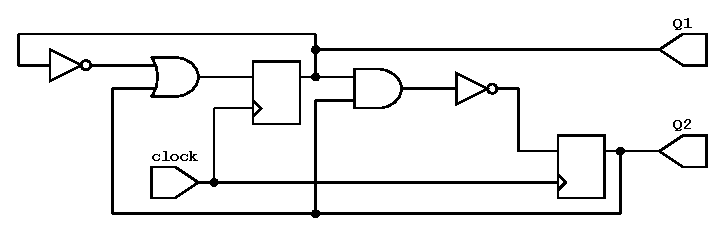
\includegraphics[width=0.85\linewidth]{figures/02_netlist.pdf}
\caption{The circuit of step 02, drawn by \cc{make svg}: two flip-flops (the
boxes with the small triangle at the clock input) and the logic between their
outputs and inputs.}
\label{fig:step02-netlist}
\end{figure}

Mathematically, the circuit is a map $\{0,1\}^2 \to \{0,1\}^2$, $(Q_1, Q_2)
\mapsto (Q_1', Q_2')$, which is applied once per clock cycle. Starting from
$(0,0)$ we get
\[
  (0,0) \mapsto (1,1) \mapsto (1,0) \mapsto (0,1) \mapsto (1,1) \mapsto (1,0)
  \mapsto \cdots
\]
After the first step, the state runs through a cycle of length three.

\section{The Description in SystemVerilog}

\svfile{02_flip_flops/test.sv}

\textbf{The combinational part} is an \cc{always_comb} block as in step 01. It
computes the two signals \cc{nextQ1} and \cc{nextQ2}, the inputs of the
flip-flops.

\textbf{\cc{always_ff} describes flip-flops.} The block
\begin{lstlisting}
always_ff @ (posedge clock) begin
    Q1 <= nextQ1;
    Q2 <= nextQ2;
end
\end{lstlisting}
says: at every rising edge (\cc{posedge}, positive edge) of \cc{clock}, \cc{Q1}
takes over the value of \cc{nextQ1}, and \cc{Q2} that of \cc{nextQ2}. Between
two rising edges they keep their values. That is the definition of a D
flip-flop with data input \cc{nextQ1}, output \cc{Q1}, and clock \cc{clock}.
So these three lines describe the two flip-flops of
Figure~\ref{fig:step02-netlist}.

\textbf{\cc{<=} is the non-blocking assignment.} In \cc{always_ff} we write
\cc{<=} instead of \cc{=}. Read \cc{Q1 <= nextQ1} as ``at the clock edge,
\cc{Q1} becomes what \cc{nextQ1} is just before the edge.'' All right-hand
sides in the block are taken from before the edge, and only then are all
flip-flops updated, at the same time. This is how real flip-flops behave: all
of them sample their inputs at the same edge.

The rule for the two kinds of blocks is simple, and we follow it in all
designs:
\begin{center}
\begin{tabular}{lll}
\toprule
block & describes & assignment \\
\midrule
\cc{always_comb} & combinational logic & \cc{=} \\
\cc{always_ff @ (posedge clock)} & flip-flops, updated at the rising edge & \cc{<=} \\
\bottomrule
\end{tabular}
\end{center}

\textbf{\cc{initial} sets the values at power-up.} The \cc{initial} block
states that \cc{Q1} and \cc{Q2} start as 0. On the FPGA this is the value the
flip-flops have right after the configuration is loaded. Our flip-flops start
with 0 anyway, so here it changes nothing on the chip, but it documents the
start state, and the simulation needs it (otherwise it would not know where to
start).

\textbf{The same type, two kinds of hardware.} \cc{nextQ1} and \cc{Q1} are
both declared as \cc{logic}. That \cc{nextQ1} becomes a wire and \cc{Q1} the
output of a flip-flop follows only from the block that assigns it. In
SystemVerilog, the hardware is determined by how a signal is used, not by its
declaration.

\begin{pitfall}
Assign every signal in \emph{one} block only. A signal that is assigned in an
\cc{always_comb} and also in an \cc{always_ff} would be the output of a gate
and of a flip-flop at the same time, two drivers on one wire. (The
\cc{initial} block is the one exception we allow ourselves: on the FPGA it sets
the power-up value of the flip-flop and drives nothing afterwards. Verilator's
linter does not know that and warns about it, see
Section~\ref{sec:step02-sim}.)
\end{pitfall}

\begin{exercise}
\label{ex:step02-blocking}
Swap the two lines in the \cc{always_ff} block. Does the circuit change? What
if the block were
\begin{lstlisting}
always_ff @ (posedge clock) begin
    Q1 <= ~Q1 | Q2;
    Q2 <= ~(Q1 & Q2);
end
\end{lstlisting}
without the \cc{always_comb} block?
\end{exercise}

\section{What yosys Makes of It}

The statistics in \cc{test.log} now list two kinds of building blocks:

\outputfile{step02_yosys_stat.txt}

An \cc{SB_DFF} is a D flip-flop, the one in a logic cell. Here is the netlist
in short, one building block per line with the signals at its connections
(\cc{C} clock, \cc{D} data input, \cc{Q} output; \cc{I0} to \cc{I3} and \cc{O}
for the LUTs):

\outputfile{step02_cells.txt}

Each next-state function became one LUT, whose output goes to the data input
of a flip-flop. Since a logic cell contains a LUT \emph{and} a flip-flop, nextpnr
puts each pair into one logic cell, and the whole design needs two of them (plus
two for the constants, as in step 01). You can check the LUTs as in
Section~\ref{sec:step01-yosys}: with \cc{Q2} on $x_3$ and \cc{Q1} on $x_2$, the
LUT of \cc{Q1} selects $t_{8Q_2 + 4Q_1}$, and its \cc{LUT_INIT} gives $t_0 = 1$,
$t_4 = 0$, $t_8 = t_{12} = 1$: that is $\neg Q_1 \vee Q_2$.

\section{How Fast May the Clock Be?}

Now there are paths from flip-flops through logic to flip-flops, and nextpnr can
say how long the slowest one takes. Its answer:

\outputfile{step02_pnr_fmax.txt}

With a clock of 232\,MHz there would still be enough time for the signal from
the output of a flip-flop through a LUT to the input of the next flip-flop. Our
board's clock has 12\,MHz, so there is plenty of room. That will change: the
ULM in Chapter~\ref{ch:step09} reaches only about 15\,MHz.

\section{Where Are the Pins?}
\label{sec:step02-pins}

nextpnr also prints warnings this time:

\outputfile{step02_pnr_warnings.txt}

The ports of this design are called \cc{clock}, \cc{Q1} and \cc{Q2}, and none
of these names is in \cc{icebreaker.pcf}. The Makefile calls nextpnr with
\cc{--pcf-allow-unconstrained}, so instead of an error we get these warnings,
and nextpnr connects the ports to \emph{some} pins. Moreover, the line
\cc{set_frequency CLK 12} in the pin file refers to \cc{CLK}, which does not
exist here, so nextpnr does not know which clock to check against. (It still
checks against 12\,MHz, its default.)

\begin{pitfall}
Port names of the top module must be names from \cc{icebreaker.pcf},
otherwise the port ends up on an arbitrary pin, and the design does nothing
visible on the board. Read the warnings of nextpnr: ``unconstrained in PCF''
always means a typo or a forgotten pin.
\end{pitfall}

To see something on the board, the ports need pin names. For the clock, the
12\,MHz oscillator \cc{CLK} is the obvious choice, but then the LEDs change
twelve million times per second, and you see them all glowing at the same time.
We need a slower clock, or a way to make something happen only once in a while.
This is what the next step is about.

\begin{exercise}
\label{ex:step02-button}
Rename the ports so that the first button is the clock and the LEDs show the
state: \cc{clock} becomes \cc{BTN1}, \cc{Q1} becomes \cc{LED1}, \cc{Q2} becomes
\cc{LED2} (also in the testbench). Program the board and press the button a few
times. Does the state always advance by one step per press?
\end{exercise}

\section{Simulation}
\label{sec:step02-sim}

The testbench now has only one input to set, the clock. Its loop inverts it in
every step:

\cpppart{firstline=21,lastline=30}{02_flip_flops/tb_test.cpp}

So the clock has a rising edge at every second step. Figure~\ref{fig:step02-waves}
shows the result of \cc{make sim} in the waveform viewer.

\begin{figure}[ht]
\centering
\begin{tikzpicture}[x=6.5mm,y=7mm]
  \foreach \name/\y in {clock/6, nextQ1/4.5, nextQ2/3, Q1/1.5, Q2/0} {
    \node[anchor=east,font=\small\ttfamily] at (-0.3,\y+0.3) {\name};
    \draw[black!8,line width=3mm] (0,\y+0.3) -- (15,\y+0.3);
  }
  % clock: 1 at t=0, toggles every step
  \draw[clocksig] (0,6.6) \foreach \t in {1,3,...,13} { -- (\t,6.6) -- (\t,6) -- (\t+1,6) -- (\t+1,6.6) } -- (15,6.6);
  % Q1: 0 until 2, 1 on [2,6), 0 on [6,8), 1 on [8,12), 0 on [12,14), 1 from 14
  \draw[signal] (0,1.5) -- (2,1.5) -- (2,2.1) -- (6,2.1) -- (6,1.5) -- (8,1.5) -- (8,2.1) -- (12,2.1) -- (12,1.5) -- (14,1.5) -- (14,2.1) -- (15,2.1);
  % Q2: 0 until 2, 1 on [2,4), 0 on [4,6), 1 on [6,10), 0 on [10,12), 1 on [12,16)
  \draw[signal] (0,0) -- (2,0) -- (2,0.6) -- (4,0.6) -- (4,0) -- (6,0) -- (6,0.6) -- (10,0.6) -- (10,0) -- (12,0) -- (12,0.6) -- (15,0.6);
  % nextQ1 = ~Q1 | Q2: 1 on [0,4), 0 on [4,6), 1 on [6,10), 0 on [10,12), 1 on [12,...)
  \draw[signal,draw=green!45!black] (0,5.1) -- (4,5.1) -- (4,4.5) -- (6,4.5) -- (6,5.1) -- (10,5.1) -- (10,4.5) -- (12,4.5) -- (12,5.1) -- (15,5.1);
  % nextQ2 = ~(Q1 & Q2): 1, 0 on [2,4), 1 on [4,8), 0 on [8,10), 1 on [10,14), 0 on [14,...)
  \draw[signal,draw=green!45!black] (0,3.6) -- (2,3.6) -- (2,3) -- (4,3) -- (4,3.6) -- (8,3.6) -- (8,3) -- (10,3) -- (10,3.6) -- (14,3.6) -- (14,3) -- (15,3);
  \foreach \t in {0,2,...,14} {
    \draw[black!12] (\t,-0.4) -- (\t,6.9);
    \node[below,font=\scriptsize] at (\t,-0.4) {\t};
  }
  \node[note,anchor=west] at (15.3,-0.7) {\cc{sim_time}};
\end{tikzpicture}
\caption{The waveforms of step 02. At every rising edge of \cc{clock} (the
gray lines), \cc{Q1} and \cc{Q2} take over the values that \cc{nextQ1} and
\cc{nextQ2} had just before.}
\label{fig:step02-waves}
\end{figure}

The simulation starts at time 0 with \cc{clock} already 1. This is not a rising
edge, since there is no earlier value, so the state stays $(0,0)$. The first
rising edge is at time 2, and from there on the state runs through $(1,1)$,
$(1,0)$, $(0,1)$, $(1,1)$, \dots, as computed above. Note how \cc{nextQ1} and
\cc{nextQ2} change right after an edge, as soon as the state has changed: they
are combinational, and they always show what the state will be after the next
edge.

Verilator prints some warnings during \cc{make sim}:
\begin{terminal}
%Warning-MULTIDRIVEN: test.sv:20:9: Variable written to in always_ff also
written by other process (IEEE 1800-2023 9.2.2.4): 'Q1'
\end{terminal}
This is the \cc{initial} block of the pitfall above. For a simulator, it is a
second process writing \cc{Q1}. For us, it is the power-up value of the
flip-flop, and we can ignore the warning.

\solutions

\solution
Swapping the lines changes nothing: both right-hand sides are taken from before
the edge, and both flip-flops are updated together. The order of the lines in
an \cc{always_ff} block with \cc{<=} does not matter.

The block without \cc{always_comb} describes the same circuit as well. The
expressions on the right are computed by combinational logic in any case; we
only no longer give its outputs names. Here, \cc{Q1} on the right of the second
line is still the old value, since \cc{<=} takes all right-hand sides from
before the edge. (With \cc{=} instead of \cc{<=}, the second line would see the
new value of \cc{Q1}, and the block would describe a different circuit. This
is why we never use \cc{=} in \cc{always_ff}.)

\solution
After renaming, nextpnr finds all ports in the pin file, and the warnings are
gone. On the board you will see the state advance, but now and then by two or
more steps per press. A mechanical button does not close cleanly: its
contacts bounce for a few milliseconds and produce several edges. For a clock,
which must be clean, a button is a bad choice. We will instead sample buttons
with the 12\,MHz clock, starting in Chapter~\ref{ch:step04}, and react to a
press only once the contacts have settled, starting in
Chapter~\ref{ch:step05}.


\part{From Counters to a Computer}
\label{part:computer}

\chapter{Step 03: A Counter on the 7-Segment Display}
\label{ch:step03}

In step 02 the clock was too fast to see anything. Step 03 solves this with a
counter: it counts the 12 million clock edges of a second and then increments
a second counter, whose value appears on the two digits of the 7-segment
display. For this we need many new pieces of SystemVerilog at once, but each
of them describes a circuit you know: signals of several bits (vectors),
constants, registers with an adder, multiplexers written as \cc{if} and
\cc{case}, and a module used as a part of another module. Everything is in the
directory \cc{03_hexdisplay}.

\section{The Circuit}
\label{sec:step03-circuit}

The design consists of three parts (Figure~\ref{fig:step03-netlist}):
\begin{itemize}
\item a counter \cc{posEdgeCount} that counts the edges of the 12\,MHz clock
  and starts again at 0 after twelve million of them;
\item a one-bit register \cc{tic}, which is 1 for exactly one clock cycle
  whenever \cc{posEdgeCount} starts again, so once per second;
\item an 8-bit counter \cc{hex_val}, which is incremented in the clock cycles
  in which \cc{tic} is 1. Its value goes to a second module, \cc{dev_hex},
  which drives the display.
\end{itemize}

\begin{figure}[ht]
\centering
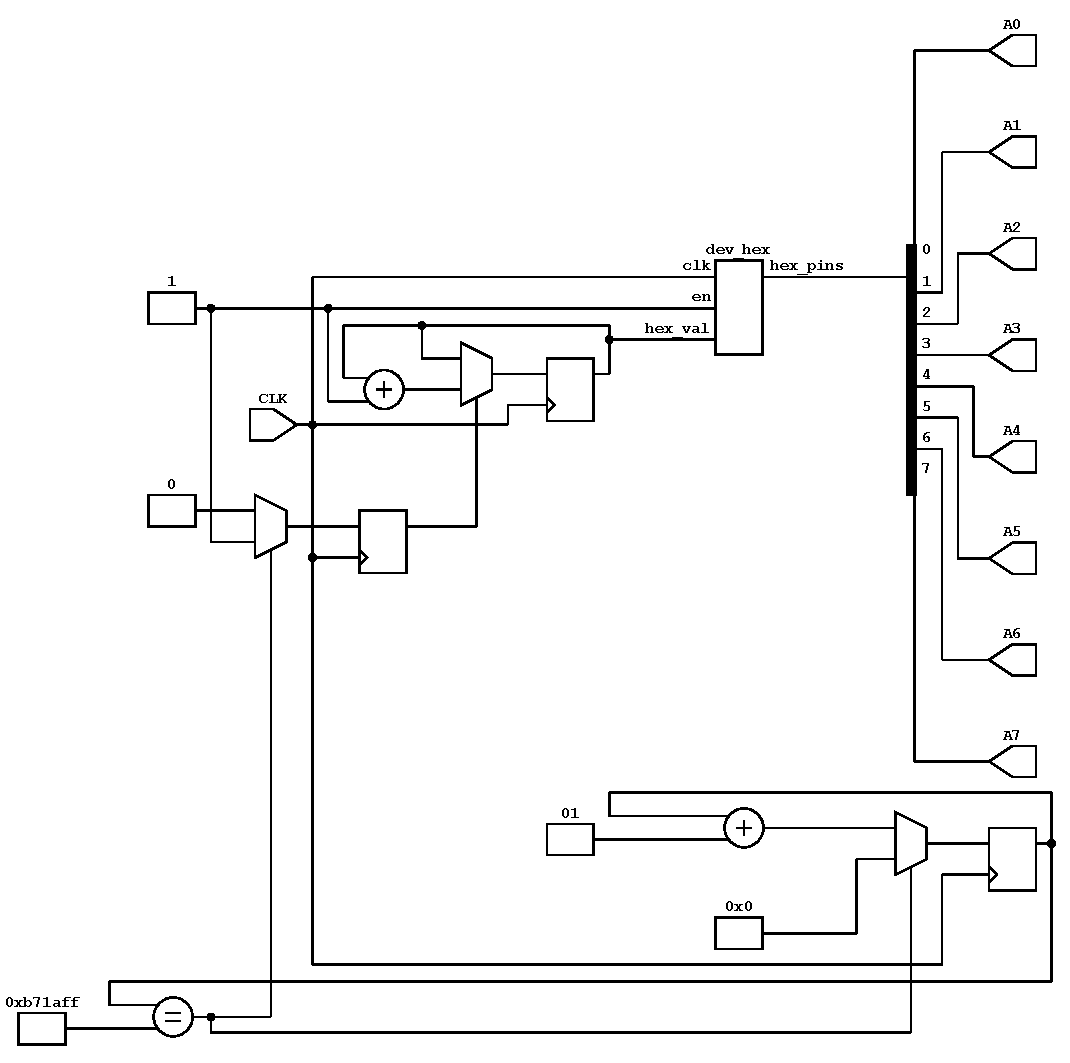
\includegraphics[width=0.8\linewidth]{figures/03_netlist.pdf}
\caption{The top module of step 03, drawn by \cc{make svg}. Bottom:
\cc{posEdgeCount} with its adder, the multiplexer that resets it and the
comparison with \cc{0xb71aff}${}= 11\,999\,999$. Middle left: \cc{tic}. Top:
\cc{hex_val} with its adder and the multiplexer that keeps the old value when
\cc{tic} is 0. The box \cc{dev_hex} is a module of its own.}
\label{fig:step03-netlist}
\end{figure}

All flip-flops in this design are clocked by the 12\,MHz clock \cc{CLK}. This
is the answer to the question at the end of Chapter~\ref{ch:step02}. We do not
build a slower clock; we build a signal that says ``now'' once per second, and
the register \cc{hex_val} takes over a new value only in those clock cycles.
Such a signal is called a \term{clock enable}. (One could also use the output
of a flip-flop as the clock of other flip-flops. But then the design has
several clocks whose edges are shifted against each other, and the tools can
no longer check the timing between them easily. We stay with one clock.)

\section{Vectors and Constants}
\label{sec:step03-vectors}

Here is the top module:

\svfile{03_hexdisplay/test.sv}

\textbf{Vectors.} \cc{logic [7:0] hex_val} declares eight signals
\cc{hex_val[7]}, \dots, \cc{hex_val[0]} under one name, a \term{vector}, like a
bus of eight wires in CircuitVerse. The range \cc{[7:0]} says that the bits are
numbered from 7 on the left down to 0 on the right. Whenever we compute with
a vector, it stands for the unsigned number
\[
  u(\mathit{hex\_val}) = \sum_{i=0}^{7} \mathit{hex\_val}_i \cdot 2^i ,
\]
so \cc{hex_val[7]} is the most significant bit. Parts of a vector are written
\cc{hex_val[3:0]} (the low four bits, a \term{nibble}) or \cc{hex_val[7:4]}
(the high nibble). In \cc{dev_hex} you will also see \cc{counter[2 +: 3]}:
three bits, starting at bit 2 and counting upward, which is the same as
\cc{counter[4:2]}. None of this is hardware; it only names wires.

\textbf{Concatenation.} Braces put signals side by side into one vector, the
first one on the left (most significant). Line 14,
\begin{lstlisting}
assign {A7, A6, A5, A4, A3, A2, A1, A0} = hex_pins;
\end{lstlisting}
has a concatenation on the left side: it splits the vector \cc{hex_pins} into
its bits, \cc{A7} gets \cc{hex_pins[7]} and \cc{A0} gets \cc{hex_pins[0]}. The
ports have to be single bits with the names from \cc{icebreaker.pcf}, where
\cc{A0} to \cc{A7} are the pins of PMOD 1A with the display. Inside, we
prefer to work with a vector. On the right side, as in \cc{dev_hex},
\cc{{digit_sel, seg_pins}} joins a bit and a 7-bit vector into 8 bits.

\textbf{Literals with a size.} A constant can be given with its number of bits
and its base: \cc{8'h0} is the number 0 as 8 bits in hexadecimal notation,
\cc{1'b1} a single 1 bit, \cc{7'b1000000} seven bits in binary, \cc{4'hA} the
four bits \cc{1010}. The format is \emph{width}\,\cc{'}\,\emph{base}\,\emph{digits}
with base \cc{b}, \cc{d} or \cc{h}. Underscores are ignored and only help
reading: \cc{12_000_000}. A number without a size, like \cc{1} or \cc{0}, has
32 bits. In hardware a constant is a wire tied to 0 or 1.

\textbf{\cc{localparam} names a constant.} \cc{localparam CLK_FREQ = 12_000_000;}
gives the number a name. It is not a signal and creates no hardware: wherever
\cc{CLK_FREQ} appears, the tools use the number. Even \cc{CLK_FREQ - 1} in
line 26 is computed by the tools, not by a subtractor: in
Figure~\ref{fig:step03-netlist} it is the constant \cc{0xb71aff} at the
comparator.

\textbf{\cc{integer}} is a 32-bit signed variable, an older type from Verilog.
In hardware, \cc{posEdgeCount} becomes 32 flip-flops, as we will see.

\textbf{Declaration with a value.} \cc{logic tic = 0;} declares \cc{tic} and
gives it the value 0 at the start. This is the same as an \cc{initial} block
(Chapter~\ref{ch:step02}): the power-up value of the flip-flops. The same
holds for \cc{posEdgeCount} and \cc{hex_val}. Verilator again reminds us that
these signals are also written in an \cc{always_ff} block:
\begin{terminal}
%Warning-PROCASSINIT: test.sv:21:17: Procedural assignment to declaration with
initial value: 'tic'
\end{terminal}
For us this is intended, as with \cc{MULTIDRIVEN} in Chapter~\ref{ch:step02}.

\section{Counters}
\label{sec:step03-counter}

\textbf{A counter is a register and an adder.} The block of lines 35--39 says:
at a rising edge of \cc{CLK}, \cc{hex_val} takes over \cc{hex_val + 1} if
\cc{tic} is 1. Read it as a circuit: an 8-bit register (eight flip-flops)
whose output goes through an adder that adds 1, and whose input is the output
of that adder. This is the counter you built in CircuitVerse.

The adder has eight output bits, so it computes modulo $2^8$:
\[
  u(\mathit{hex\_val}') = \bigl(u(\mathit{hex\_val}) + 1\bigr) \bmod 2^8 ,
\]
and after \cc{8'hff} comes \cc{8'h00}. (Strictly, \cc{hex_val + 1} has 32 bits,
because the literal \cc{1} has 32 bits. Assigning it to the 8-bit \cc{hex_val}
drops the upper 24 bits, and the result is the same.)

\textbf{\cc{if} in \cc{always_ff} is a multiplexer.} What happens if \cc{tic}
is 0? The block does not say, and for a flip-flop that means: it keeps its
value. So in front of the data input of the register there is a multiplexer
(Figure~\ref{fig:step03-netlist}, top) that selects between the new value
\cc{hex_val + 1} and the old value \cc{hex_val}, and \cc{tic} is its select
input. A register whose next value is either a new value or its old one,
depending on a signal, is a register with an \term{enable}, and the iCE40 has
a flip-flop for exactly this, \cc{SB_DFFE}. Mathematically,
\[
  \mathit{hex\_val}' =
  \begin{cases}
    \mathit{hex\_val} + 1, & \text{if } \mathit{tic} = 1,\\
    \mathit{hex\_val}, & \text{otherwise.}
  \end{cases}
\]

\textbf{Several assignments: the last one wins.} The block of lines 23--30
assigns \cc{posEdgeCount} and \cc{tic} twice:
\begin{lstlisting}
posEdgeCount <= posEdgeCount + 1;
tic <= 0;
if (posEdgeCount == CLK_FREQ - 1) begin
    posEdgeCount <= 0;
    tic <= 1;
end
\end{lstlisting}
The rule is: of all assignments to a signal in a block that apply, the last
one counts. So \cc{posEdgeCount} becomes 0 if it equals \cc{CLK_FREQ - 1}, and
\cc{posEdgeCount + 1} otherwise. And \cc{tic} becomes 1 in that case and 0
otherwise, in short $\mathit{tic}' = (u(\mathit{posEdgeCount}) =
11\,999\,999)$. This is a description of next-state functions, not a sequence
of steps: the comparison \cc{==} is a comparator circuit, the \cc{if} is a
multiplexer behind the adder, and both flip-flops take over their new values
at the same edge, as in Chapter~\ref{ch:step02}.

So \cc{posEdgeCount} runs through $0, 1, \dots, 11\,999\,999, 0, 1, \dots$,
twelve million values, and \cc{tic} is 1 in the clock cycle right after
\cc{posEdgeCount} was $11\,999\,999$: once every $12\,000\,000$ cycles,
exactly once per second. A counter that produces such a pulse once every $N$ cycles is
a \term{clock divider}, even though no new clock comes out of it.

\begin{exercise}
\label{ex:step03-period}
An earlier version of \cc{test.sv} compared with \cc{CLK_FREQ} instead of
\cc{CLK_FREQ - 1}. How many clock cycles lay between two cycles in which
\cc{tic} was 1, and how long was the ``second'' of that design? Would you
have noticed on the board?
\end{exercise}

\section{Using a Module: dev\_hex}
\label{sec:step03-instance}

Lines 41--46 place the display driver into our design:
\begin{lstlisting}
dev_hex dev_hex0 (
    .clk(CLK),
    .en(1'b1),
    .hex_val(hex_val),
    .hex_pins(hex_pins)
);
\end{lstlisting}
This is an \term{instance} of the module \cc{dev_hex}: a copy of the circuit
described in \cc{dev_hex.sv}, named \cc{dev_hex0}, with its ports connected to
our signals. In CircuitVerse terms, we place a subcircuit and wire it up.
\cc{.clk(CLK)} connects the port \cc{clk} of the instance to our signal
\cc{CLK}. Connecting by name is safer than by position, and we always do it.
The port \cc{en} is connected to the constant 1: the display is always on. We
could place several instances of the same module, each with its own name and
its own flip-flops.

The Makefile passes all \cc{.sv} files of the directory to the tools
(\cc{SV_FILES := $(wildcard *.sv)}), so \cc{dev_hex.sv} is found without
further ado; which module is the top module is given by \cc{-top test}.

\section{Driving the 7-Segment Display}
\label{sec:step03-display}

Each digit of the display consists of seven LED segments, called $a$ to $g$
(Figure~\ref{fig:step03-segments}). The module has only eight signal lines,
not $2 \cdot 7$: the seven segment lines are shared by both digits, and the
eighth line selects which of the two digits is switched on. So at any moment
at most one digit shows something. To show two digits, the driver alternates
between them, so fast that the eye sees both at once. This is called
\term{multiplexing} a display.

\begin{figure}[ht]
\centering
\begin{tikzpicture}[scale=0.55,
    seg/.style={line width=4pt,line cap=round,draw=red!75!black},
    lbl/.style={font=\small}]
  % one digit, segment a at the top, g in the middle
  \draw[seg] (0.3,4) -- (1.7,4);   \node[lbl,above] at (1,4.2) {$a$};
  \draw[seg] (2,3.7) -- (2,2.3);   \node[lbl,right] at (2.2,3) {$b$};
  \draw[seg] (2,1.7) -- (2,0.3);   \node[lbl,right] at (2.2,1) {$c$};
  \draw[seg] (0.3,0) -- (1.7,0);   \node[lbl,below] at (1,-0.2) {$d$};
  \draw[seg] (0,1.7) -- (0,0.3);   \node[lbl,left] at (-0.2,1) {$e$};
  \draw[seg] (0,3.7) -- (0,2.3);   \node[lbl,left] at (-0.2,3) {$f$};
  \draw[seg] (0.3,2) -- (1.7,2);   \node[lbl,above] at (1,2.1) {$g$};
  \node[anchor=west,align=left,font=\small] at (4.5,2) {%
    \begin{tabular}{@{}l@{}}
    \cc{seg_pins[0]} = $a$, \dots, \cc{seg_pins[6]} = $g$\\[2pt]
    0 = segment on, 1 = segment off\\[2pt]
    \cc{hex_pins} = \cc{{digit_sel, seg_pins}}, pins \cc{A7}, \dots, \cc{A0}
    \end{tabular}};
\end{tikzpicture}
\caption{The segments of one digit, and how \cc{dev_hex} encodes them.}
\label{fig:step03-segments}
\end{figure}

\subsection*{The segments: a truth table}

Which segments show a hexadecimal digit is a function
$\{0,1\}^4 \to \{0,1\}^7$, and the last block of \cc{dev_hex.sv} is its truth
table:

\svpart{firstline=58,lastline=77}{03_hexdisplay/dev_hex.sv}

\textbf{\cc{case} selects by value.} The \cc{case} statement compares
\cc{digit} with each of the values on the left and applies the assignment of
the matching one. In an \cc{always_comb} block it describes combinational
logic, here literally a table with 16 rows and 7 output columns. The bits are
written from \cc{segments[6]} ($g$) on the left to \cc{segments[0]} ($a$) on
the right, and a 0 switches a segment on. For example, \cc{4'h1} gives
\cc{1111001}: only $b$ and $c$ are on, the two segments on the right, which
form a ``1''. And \cc{4'h8} gives \cc{0000000}, all segments on.

Every segment is a Boolean function of the four bits of \cc{digit}. A function
of four bits is exactly what one LUT computes (Section~\ref{sec:lut}), so the
whole table becomes seven LUTs, one per segment.

\begin{pitfall}
A \cc{case} in \cc{always_comb} must assign a value in \emph{every} case.
Here it does: all 16 values of a 4-bit \cc{digit} are listed. If a case were
missing, the output would have to keep its old value for that input, and a
combinational circuit cannot keep anything. The tools then build a
\term{latch}, a storage element without a clock, which is almost never what
you want. Assigning a default value first, as the block that computes
\cc{digit} does with \cc{digit = 0;}, avoids this. In \cc{always_ff}, by contrast, a missing assignment is fine:
the flip-flop keeps its value, as we saw with \cc{hex_val}.
\end{pitfall}

\subsection*{Multiplexing the two digits}

The rest of \cc{dev_hex} decides which digit is shown when:

\svpart{firstline=13,lastline=46}{03_hexdisplay/dev_hex.sv}

\textbf{A counter as a time base.} \cc{counter} is a 30-bit counter that is
incremented at every clock edge. Only its bits 4 to 2 are used: line 17
connects them to \cc{display_state}. They change every 4 clock cycles and run through
$0, 1, \dots, 7$ once every 32 cycles, which is the 375\,kHz of the comment
($12\,\text{MHz} / 32$). yosys notices that bits 5 to 29 are never used and
removes them, so only five flip-flops remain. (\cc{always @(posedge clk)} is
the older Verilog form of \cc{always_ff @ (posedge clk)}, and describes the same
flip-flops here.)

\textbf{Which nibble.} The next block is a multiplexer:

\svpart{firstline=48,lastline=56}{03_hexdisplay/dev_hex.sv}

In states 0 and 1, \cc{digit} is the low nibble \cc{hex_val[3:0]},
in states 4 and 5 the high nibble, otherwise 0.

\textbf{When.} The \cc{case} in the clocked block sets the registers
\cc{seg_pins} and \cc{digit_sel} depending on the state:
\begin{center}
\begin{tabular}{cll}
\toprule
\cc{display_state} & \cc{seg_pins} & \cc{digit_sel} \\
\midrule
0, 1 & segments of the low nibble & (keeps 1) \\
2 & all off (\cc{~0}) & \\
3 & & becomes 0 \\
4, 5 & segments of the high nibble & (keeps 0) \\
6 & all off & \\
7 & & becomes 1 \\
\bottomrule
\end{tabular}
\end{center}
(\cc{~0} inverts the 32-bit number 0, and the lower 7 bits of the result, all
ones, go into \cc{seg_pins}.) Figure~\ref{fig:step03-mux} shows one period.
While \cc{digit_sel} is 1 the display shows the low nibble, which must
therefore be the right digit; while it is 0, the high nibble on the left. The
select line changes only in states 3 and 7, while all segments are off. If it
changed while segments were on, the other digit would light up briefly with
the wrong pattern, a faint ``ghost''. Each digit is on for 8 of the 32 cycles,
the 25\,\% duty cycle of the comment.

\begin{figure}[ht]
\centering
\begin{tikzpicture}[x=3.3mm,y=6mm]
  \def\bus#1#2#3#4{% x1, x2, y, label
    \draw[signal] (#1+0.25,#3) -- (#2-0.25,#3) -- (#2,#3+0.3) -- (#2-0.25,#3+0.6)
      -- (#1+0.25,#3+0.6) -- (#1,#3+0.3) -- cycle;
    \node[font=\scriptsize] at ({(#1+#2)/2},#3+0.3) {#4};}
  \foreach \t in {0,4,...,32} {
    \draw[black!12] (\t,0.8) -- (\t,6.9);
    \node[below,font=\scriptsize] at (\t,0.8) {\t};
  }
  \foreach \name/\y in {CLK/6, display\_state/4.8, seg\_pins/3.6, digit\_sel/2.4, shown/1.2} {
    \node[anchor=east,font=\small\ttfamily] at (-0.3,\y+0.3) {\name};
  }
  \draw[clocksig] (0,6) \foreach \t in {0,...,33} { -- (\t,6) -- (\t,6.6) -- (\t+0.5,6.6) -- (\t+0.5,6) } -- (34,6);
  \foreach \s in {0,...,7} { \bus{4*\s}{4*\s+4}{4.8}{\s} }
  \bus{32}{34}{4.8}{0}
  \bus{0}{1}{3.6}{}
  \bus{1}{9}{3.6}{low nibble}
  \bus{9}{17}{3.6}{off}
  \bus{17}{25}{3.6}{high nibble}
  \bus{25}{33}{3.6}{off}
  \bus{33}{34}{3.6}{}
  \draw[signal] (0,3) -- (13,3) -- (13,2.4) -- (29,2.4) -- (29,3) -- (34,3);
  \bus{1}{9}{1.2}{right digit}
  \bus{17}{25}{1.2}{left digit}
  \node[note,anchor=north east] at (34,0.3) {clock cycles};
\end{tikzpicture}
\caption{One period of \cc{dev_hex}, 32 clock cycles. The registers
\cc{seg_pins} and \cc{digit_sel} change one clock edge after
\cc{display_state} enters a new state. ``shown'' is what lights up.}
\label{fig:step03-mux}
\end{figure}

\begin{pitfall}
Lines 16 and 17 declare \cc{display_state} and connect it with \cc{assign}.
An earlier version of \cc{dev_hex.sv} did both in one line,
\begin{lstlisting}
logic [2:0] display_state = counter[2 +: 3];
\end{lstlisting}
which looks like a connection, but by the rules of SystemVerilog it is a
declaration with an initial value, like \cc{logic tic = 0;} in \cc{test.sv}:
\cc{display_state} gets the value of \cc{counter[4:2]} once at the start and
keeps it. Verilator follows this rule: in \cc{make sim}, \cc{display_state}
stayed 0 while \cc{counter} counted, so the simulated display never switched
digits. yosys (via sv2v) treated the line as a connection, and on the board
the display worked. Simulation and hardware disagreed, and neither tool
warned. A declaration with a value is a power-up value; to connect, write
\cc{assign}. (The same version also used \cc{segments} in the clocked block
before declaring it further down. The tools accepted that, but a name should
be declared before it is used, as lines 19 and 20 do now.)
\end{pitfall}

\section{What yosys Makes of It}
\label{sec:step03-yosys}

yosys flattens the design: the instance \cc{dev_hex0} disappears as a box, and
its parts appear in the netlist with names that begin with \cc{dev_hex0.}. The
statistics:

\outputfile{step03_yosys_stat.txt}

There are now four kinds of flip-flops, all of them the flip-flop of a logic
cell with extra inputs: \cc{E} (enable), \cc{R} (reset to 0) and \cc{S} (set to
1). Reset and set are \emph{synchronous}, they act at the clock edge like the
data input. With the cell names from \cc{test.json} we can tell what each one
is:
\begin{center}
\begin{tabular}{rll}
\toprule
count & type & signals \\
\midrule
32 & \cc{SB_DFFSR}, with synchronous reset & \cc{posEdgeCount} \\
8 & \cc{SB_DFFE}, with enable & \cc{hex_val}, enabled by \cc{tic} \\
7 & \cc{SB_DFFESS}, with enable and synchronous set & \cc{seg_pins} \\
7 & \cc{SB_DFF}, plain & \cc{counter[4:0]}, \cc{digit_sel}, \cc{tic} \\
\bottomrule
\end{tabular}
\end{center}
The \cc{if} that resets \cc{posEdgeCount} became the \cc{R} input: when
the comparator says ``equal'', the flip-flops become 0 at the next edge. The
``all off'' of \cc{seg_pins} became the \cc{S} input. All 32 bits of the
\cc{integer} are there, although $12\,000\,000 < 2^{24}$ and the upper 8 bits
are always 0; yosys cannot know that (Exercise~\ref{ex:step03-width}).

\subsection*{Adders and the carry chain}

The 39 \cc{SB_CARRY} belong to the three adders: 30 to the 32-bit
\cc{posEdgeCount}, 6 to the 8-bit \cc{hex_val}, 3 to the 5 remaining bits of
\cc{counter}. Here is the netlist of the counter \cc{hex_val}, one building
block per line, with the generated net names abbreviated: \cc{d[i]} is the data
input of the flip-flop of bit $i$ and \cc{c[i]} the carry into bit $i$:

\outputfile{step03_counter_cells.txt}

Read it as a ripple-carry adder for $h + 1$, with $h$ = \cc{hex_val}. Adding
1 means: bit $i$ flips if all bits below it are 1. With the carry $c_i$ into
bit $i$,
\[
  c_0 = 1, \qquad
  d_i = h_i \xor c_i, \qquad
  c_{i+1} = h_i \wedge c_i .
\]
For bit 0 this is $d_0 = \neg h_0$, a LUT that inverts (\cc{LUT_INIT} 1 for
$h_0 = 0$), and the carry into bit 1 is $h_0$ itself. For every other bit, a
LUT computes $h_i \xor c_i$ (\cc{0110100110010110} is the XOR of all four
inputs, two of which are 0), and an \cc{SB_CARRY} computes the carry. An
\cc{SB_CARRY} computes the carry of a full adder, $I_0 I_1 \vee (I_0 \vee
I_1)\,\mathit{CI}$, which is $h_i \wedge c_i$ for $I_0 = 0$.

The \cc{SB_CARRY} is not a LUT. It is a small piece of fixed logic in every
logic cell, next to the LUT, with a direct wire to the logic cell above it in
the same column. These wires form the \term{carry chain}. nextpnr places the
bits of an adder in consecutive logic cells of one column, so that the carry
runs up the chain without using the general routing.

\section{What nextpnr Makes of It}
\label{sec:step03-pnr}

\outputfile{step03_pnr_util.txt}

75 logic cells. \cc{SB_GB} is one of the eight \term{global buffers}: the
clock reaches all flip-flops over a special network with little delay
difference between them, and nextpnr puts \cc{CLK} on it.

The slowest path now starts at \cc{posEdgeCount[0]} and runs along the carry
chain to the top bit:

\outputfile{step03_pnr_path.txt}

Each step along the chain takes 0.28\,ns, and the positions show the chain
climbing the column $x = 4$ from tile $(4,1)$ to tile $(4,4)$: eight logic
cells per tile, four tiles for 32 bits. 30 steps of 0.28\,ns are the largest
part of the 15.32\,ns. The maximal clock frequency, 65\,MHz, is still far
above our 12\,MHz. But we see a rule: the longer an adder, the slower the
design. In the ULM, with its 64-bit adder, this will matter.

\begin{exercise}
\label{ex:step03-width}
Declare \cc{posEdgeCount} as \cc{logic [23:0]} instead of \cc{integer}. Why
are 24 bits enough? Predict the changes in the statistics of yosys, then check
them, and look at the logic cells and the maximal frequency in the output of
nextpnr.
\end{exercise}

\section{Simulation}
\label{sec:step03-sim}

The testbench toggles the clock, 35 rising edges in all. That is enough to
see \cc{posEdgeCount} and \cc{counter} count in the waveform viewer, and to
see the display switch digits: after each rising edge, the testbench compares
the output \cc{A7}, which is \cc{digit_sel}, with its value one edge before,
and counts the changes. At the end it prints the count, and if \cc{digit_sel}
never changed, it ends with an error, so that \cc{make sim} fails. This is
exactly the check that would have caught the mistake of the pitfall above.
\cc{tic}, however, would need twelve million edges. For a simulation we make
the second shorter:

\begin{exercise}
\label{ex:step03-sim}
Set \cc{CLK_FREQ} to 2 and \cc{MAX_SIM_TIME} in \cc{tb_test.cpp} to 200, and
run \cc{make sim}. Predict at which clock edges \cc{tic} is 1 and when
\cc{hex_val} changes, and check it in the waveform viewer. Then look at
\cc{display_state}, \cc{digit_sel} and \cc{seg_pins}, and compare with
Figure~\ref{fig:step03-mux}.
\end{exercise}

(Remember to undo the change of \cc{CLK_FREQ} before you program the board.)

\section{What Is Next}

The board now shows a number, and we know how to make something happen at a
human pace with a 12\,MHz clock. The display driver \cc{dev_hex} stays with us
until the last step. What is still missing is input: in step 04, the number on
the display comes from the DIP switch, stored into a register at the press of
a button.

\solutions

\solution
With \cc{== CLK_FREQ}, \cc{posEdgeCount} ran through $0, 1, \dots,
12\,000\,000$ and then started again at 0. These are $12\,000\,001$ values, so
\cc{tic} was 1 every $12\,000\,001$ cycles, and the second was one clock
cycle, $83$\,ns, too long. On the board nobody notices: after a day, the
display is 7\,ms behind. A counter that starts at 0 and should produce a pulse
every $N$ cycles has to start again after $N - 1$; such off-by-one errors are
found by counting in a simulation, not by watching the board.

\solution
The counter never exceeds $11\,999\,999 < 2^{24} = 16\,777\,216$, so 24 bits
hold all its values. With \cc{logic [23:0]}, yosys reports 24 \cc{SB_DFFSR}
instead of 32, 31 \cc{SB_CARRY} instead of 39 (8 fewer bits of the adder),
and 58 \cc{SB_LUT4} instead of 69. nextpnr then needs 64 logic cells instead of
75, and the maximal frequency rises from 65\,MHz to about 76\,MHz, because the
carry chain is 8 steps shorter.

\solution
With \cc{CLK_FREQ} = 2, \cc{posEdgeCount} runs through 0, 1, so \cc{tic}
is 1 in every second clock cycle, and \cc{hex_val} is incremented at the edge
that ends such a cycle: 1, 2, 3, \dots\ at every second edge.
\cc{display_state} changes every 4 cycles, \cc{seg_pins} shows the segments
of the low nibble, all ones, the segments of the high nibble, all ones, and
\cc{digit_sel} becomes 0 and 1 in the middle of the ``off'' phases, as in
Figure~\ref{fig:step03-mux}. (Since \cc{hex_val} now changes every two
cycles, the segments shown in one phase are those of the value when the phase
began, and may change during the phase.)

\chapter{Step 04: Storing the DIP Switch}
\label{ch:step04}

Step 03 showed a number on the display; now we choose the number ourselves.
The design of \cc{04_dip_switch} reads eight bits from a DIP switch and stores
them in an 8-bit register when the first button is pressed. The display shows
the register. There is almost no new SystemVerilog in this step. What is new is
that a button controls a register, and after the bouncing button at the end
of Chapter~\ref{ch:step02} we look closely at what this means.

\section{The Circuit}
\label{sec:step04-circuit}

A DIP switch is a row of eight small switches, each one giving a constant bit
for as long as we leave it alone. It sits on its own PMOD module, here on
PMOD 1B, next to the display on PMOD 1A (Figure~\ref{fig:step04-board}).

\begin{figure}[ht]
\centering
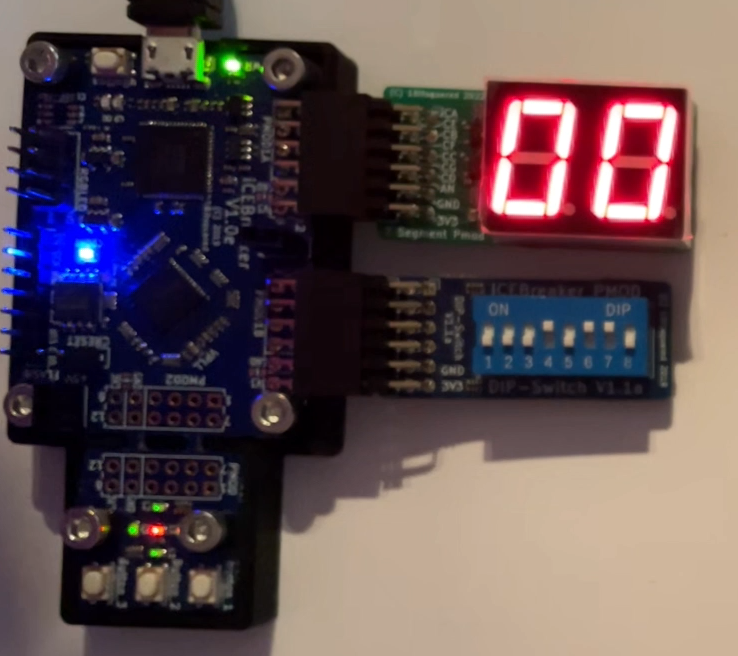
\includegraphics[width=0.55\linewidth]{figures/04_board.png}
\caption{The board with the 7-segment display (PMOD 1A, top right), the DIP
switch (PMOD 1B, right) and the module with buttons and LEDs (PMOD 2,
bottom). The display shows \cc{00}, the power-up value of the register.}
\label{fig:step04-board}
\end{figure}

The circuit is an 8-bit register with enable. Its data inputs are the switches,
its enable is the button:
\[
  \mathit{hex\_val}' =
  \begin{cases}
    \mathit{hex\_in}, & \text{if } \mathit{BTN1} = 1,\\
    \mathit{hex\_val}, & \text{otherwise,}
  \end{cases}
\]
and \cc{dev_hex} from Chapter~\ref{ch:step03} shows \cc{hex_val}.

\section{The Description in SystemVerilog}
\label{sec:step04-sv}

\svfile{04_dip_switch/test.sv}

Every piece of this was introduced in Chapter~\ref{ch:step03}. The file
\cc{dev_hex.sv} in this directory is a link to the one of step 03, so both
steps use the same display driver.

\textbf{The bit order.} Line 26 collects the eight switch inputs into a
vector, with \cc{B0} on the left:
\begin{lstlisting}
assign hex_in = {B0, B1, B2, B3, B4, B5, B6, B7};
\end{lstlisting}
So \cc{B0} is \cc{hex_in[7]}, the most significant bit, and \cc{B7} is
\cc{hex_in[0]}. If \cc{B0} to \cc{B7} are the switches 1 to 8 from left to
right, the switches read as the binary number from left to right, the way we
write numbers. (The concatenation makes this possible without a single gate:
it only decides which wire is which bit.)

\textbf{The register.} The \cc{always_ff} block in lines 30--34 is the
register with enable of Section~\ref{sec:step04-circuit}: \cc{if (BTN1)}
loads, and without an \cc{else} the register keeps its value. This is the
same construction as \cc{hex_val} in step 03, only with \cc{hex_in} instead of
\cc{hex_val + 1}, and with the button instead of \cc{tic}.

\section{What yosys Makes of It}
\label{sec:step04-yosys}

\outputfile{step04_yosys_stat.txt}

Compared with step 03, the one-second counter is gone (no \cc{SB_DFFSR}, 36
fewer \cc{SB_CARRY}), and what is left besides \cc{dev_hex} is the register. Its
eight flip-flops in the netlist:

\outputfile{step04_cells.txt}

This is as direct as it gets. Each switch goes straight into the data input
\cc{D} of a flip-flop, and the button straight into all eight enable inputs
\cc{E}. There is no LUT between them: the multiplexer of the \cc{if} is the
enable of the \cc{SB_DFFE}. (The yosys option \cc{-dffe_min_ce_use 4} in the
Makefile says to use the enable input only if at least four flip-flops share
the same enable signal; for a single flip-flop like \cc{digit_sel} in
\cc{dev_hex}, yosys builds the multiplexer with a LUT instead.)

The flip-flops are clocked by \cc{CLK}, not by the button. This is the
difference to the experiment of Exercise~\ref{ex:step02-button}, where the
button \emph{was} the clock.

\section{The Button}
\label{sec:step04-button}

In Exercise~\ref{ex:step02-button}, the state sometimes advanced by two or more
steps per press, because the contacts of the button bounce: for a few
milliseconds after we press it (and again when we release it), the signal
jumps between 0 and 1 several times. Each of these jumps was a clock edge.

Here, \cc{BTN1} is not a clock. At every edge of the 12\,MHz clock, the
register looks at the button. Pressing it for a tenth of a second means that
\cc{BTN1} is 1 at about 1.2 million clock edges, and at each of them the
register loads the switches. During the bouncing, the enable goes on and off a
few times, and the register loads in some cycles and not in others.

None of this matters, because loading is \emph{idempotent}: loading the same
value twice gives the same result as loading it once. Let $L_s$ be the map
``load $s$'', $L_s(h) = s$ for every register value $h$. Then $L_s \circ L_s =
L_s$, and whether the register loads once, three times or a million times
during a press, it ends up with $s$, the setting of the switches. In step 02
the map applied per edge was the next-state map of the state machine, and
applying it twice is not the same as applying it once. That is why bouncing
mattered there and does not matter here.

\textbf{Is the button synchronised?} No. The button changes whenever we press
it, not in step with the clock, and its signal goes straight into the enable
inputs of eight flip-flops. If it changes just before a clock edge, it may
reach some of the eight flip-flops in time and others not, and in rare cases a
flip-flop may even need a little longer than usual to decide between 0 and 1
(\term{metastability}). Usually one samples such an input with two flip-flops
in a row first, a \term{synchroniser}, and uses only the output of the second
one. Here we can do without: if some flip-flops load at the edge where the
press begins and others do not, they all load at the next edge, 83\,ns later.
And when the button is released, all eight bits already hold the setting of
the switches, so it does not matter which of them load once more.

\begin{exercise}
\label{ex:step04-change}
Press the button, and while you keep it pressed, change a switch. What does
the display do? What happens if you change a switch while the button is not
pressed?
\end{exercise}

\begin{exercise}
\label{ex:step04-count}
Suppose we want to count the presses of \cc{BTN1} instead: \cc{hex_val} is
incremented by one per press. Why does \cc{if (BTN1) hex_val <= hex_val + 1;}
not work? Describe a circuit that produces a pulse of one clock cycle when
the (synchronised) button changes from 0 to 1, write it in SystemVerilog, and
say what bouncing does to it.
\end{exercise}

\section{What nextpnr Makes of It}
\label{sec:step04-pnr}

\outputfile{step04_pnr_util.txt}

29 logic cells: the eight flip-flops of the register and \cc{dev_hex}.
18 \cc{SB_IO}: the clock, the button, eight switches, eight display pins.
nextpnr finds all of them in \cc{icebreaker.pcf}, which has a section for
the DIP switch:
\begin{terminal}
# for DIP switch
set_io -nowarn B0         43
set_io -nowarn B1         38
...
set_io -nowarn B7         28
\end{terminal}
These are the same pins as \cc{P1B1} to \cc{P1B4} and \cc{P1B7} to \cc{P1B10}
further down in the file, the signal pins of PMOD 1B. (A PMOD connector has
twelve pins in two rows; in each row, one pin is ground and one is 3.3\,V,
which leaves eight signals, numbered 1--4 and 7--10.) So, as in
Section~\ref{sec:step02-pins}, there is no warning about unconstrained pins.

\section{Simulation}
\label{sec:step04-sim}

The testbench changes the inputs at the falling edges of the clock, half a
cycle before the rising edge that samples them:

\cpppart{firstline=27,lastline=62}{04_dip_switch/tb_test.cpp}

\cc{posedge_cnt + 1} is the number of the next rising edge. For the 5th
rising edge it sets \cc{B0} and \cc{B1} and presses the button, for the 8th
it sets only \cc{B1} with the button, for the 11th it sets \cc{B0} and
\cc{B7} without the button. Figure~\ref{fig:step04-waves} shows the result of
\cc{make sim}.

\begin{figure}[ht]
\centering
\begin{tikzpicture}[x=5mm,y=6mm]
  \def\bus#1#2#3#4{% x1, x2, y, label
    \draw[signal] (#1+0.2,#3) -- (#2-0.2,#3) -- (#2,#3+0.3) -- (#2-0.2,#3+0.6)
      -- (#1+0.2,#3+0.6) -- (#1,#3+0.3) -- cycle;
    \node[font=\scriptsize\ttfamily] at ({(#1+#2)/2},#3+0.3) {#4};}
  \foreach \t in {0,2,...,24} {
    \draw[black!12] (\t,0.8) -- (\t,5.7);
    \node[below,font=\scriptsize] at (\t,0.8) {\t};
  }
  \foreach \name/\y in {CLK/4.8, BTN1/3.6, hex\_in/2.4, hex\_val/1.2} {
    \node[anchor=east,font=\small\ttfamily] at (-0.3,\y+0.3) {\name};
  }
  % CLK: 1 at even times, 0 at odd times
  \draw[clocksig] (0,5.4) \foreach \t in {0,2,...,24} { -- (\t,5.4) -- (\t+1,5.4) -- (\t+1,4.8) -- (\t+2,4.8) -- (\t+2,5.4) } -- (26,5.4);
  \draw[signal] (0,3.6) -- (7,3.6) -- (7,4.2) -- (9,4.2) -- (9,3.6) -- (13,3.6)
     -- (13,4.2) -- (15,4.2) -- (15,3.6) -- (26,3.6);
  \bus{0}{7}{2.4}{00} \bus{7}{9}{2.4}{c0} \bus{9}{13}{2.4}{00}
  \bus{13}{15}{2.4}{40} \bus{15}{19}{2.4}{00} \bus{19}{21}{2.4}{81}
  \bus{21}{26}{2.4}{00}
  \bus{0}{8}{1.2}{00} \bus{8}{14}{1.2}{c0} \bus{14}{26}{1.2}{40}
  \node[note,anchor=north east] at (26,0.3) {\cc{sim_time}};
\end{tikzpicture}
\caption{The waveforms of step 04 (values in hexadecimal). The inputs change
at falling edges. \cc{hex_val} takes over \cc{hex_in} at the rising edges at
which \cc{BTN1} is 1, and ignores \cc{hex_in} otherwise.}
\label{fig:step04-waves}
\end{figure}

The inputs change at time 7, and \cc{hex_val} becomes \cc{c0} =
\cc{11000000} at the rising edge at time 8: \cc{B0} and \cc{B1} are the two
most significant bits. It becomes \cc{40} at time 14, and at time 20 nothing
happens, since the button is not pressed.

\begin{pitfall}
An earlier version of the testbench set the inputs at the rising edges, in
the same step as the clock, before \cc{eval()}. Then an input and the clock
change at the same moment, and whether the flip-flops see the old or the new
input at that edge is a race. Verilator let them see the new inputs, so
\cc{hex_val} changed at the very edge at which the inputs changed. On a real
chip, an input that changes together with the clock edge violates the
\term{setup time}, the short time before the edge during which the input of a
flip-flop must be stable. A testbench should change its inputs away from the
active edge, for example at the falling edge, as this one does now.
\end{pitfall}

\section{What Is Next}

We now have input (the switches), storage (a register), and output (the
display). Step 05 adds the missing piece of a computer, arithmetic: four
registers, an adder/subtractor and status flags, controlled by instructions
that we set on the DIP switch.

\solutions

\solution
While the button is pressed, the register loads the switches at every clock
edge, so the display follows the switches at once: the register behaves like
a wire from the switches to the display. When you release the button, the
register keeps the last setting. Without the button, the switches have no
effect at all.

\solution
\cc{if (BTN1) hex_val <= hex_val + 1;} increments at every clock edge while the
button is pressed, about 1.2 million times for a press of a tenth of a
second. We must react to the \emph{change} of the button, not to its level.
For this we remember the value of the button from the cycle before: a press
begins in the cycle in which the button is 1 now and was 0 one cycle before.
As a circuit: a synchroniser of two flip-flops, a third flip-flop that delays
by one cycle, and an AND gate with an inverted input:
\begin{lstlisting}
logic btn_s1 = 0, btn_s2 = 0, btn_prev = 0;

always_ff @ (posedge CLK) begin
    btn_s1   <= BTN1;       // synchroniser, first stage
    btn_s2   <= btn_s1;     // synchroniser, second stage
    btn_prev <= btn_s2;     // value one clock earlier
end

logic press;
assign press = btn_s2 & ~btn_prev;

always_ff @ (posedge CLK) begin
    if (press) begin
        hex_val <= hex_val + 1;
    end
end
\end{lstlisting}
\cc{press} is 1 for exactly one cycle per rising edge of \cc{btn_s2}. But
bouncing produces several rising edges per press, and each of them is
counted: we are back at the problem of Exercise~\ref{ex:step02-button},
because incrementing is not idempotent. The remedy is a \term{debouncer}:
accept a new value of the button only after it has been stable for some
milliseconds, for example with a counter that counts the cycles in which the
synchronised button differs from the accepted value, is reset to 0 as soon as
they agree again, and copies the new value when it reaches $2^{17}$ (about
11\,ms at 12\,MHz). Step 05 uses exactly this circuit for its button
(Section~\ref{sec:step05-button}).

\chapter{Step 05: A Mini-ALU}
\label{ch:step05}

% Listings with line numbers, for listings whose lines the text refers to.
\lstdefinestyle{numbered}{numbers=left,numberstyle=\tiny\color{codecomment},numbersep=6pt}

% Inline code that contains a percent sign, such as a register name \ccpct{%1}.
\providecommand{\ccpct}{\begingroup\catcode`\%=12 \ccpctaux}
\providecommand{\ccpctaux}[1]{\cc{#1}\endgroup}

With step 05 the board starts to compute. The design of \cc{05_mini_alu} is
the Mini-ALU that we build in CircuitVerse in the course HPC0 (worksheets 4
and 6): four 8-bit registers, one of them the zero register, an
adder/subtractor, four status flags and a decoder. It executes 8-bit
instructions that we set on the DIP switch, one per press of a button. The
new pieces of SystemVerilog are the array, four registers under one name
selected by a signal, and the replication \cc{{8{sub}}}. And for the first
time we react to a button press rather than to the level of the button, with
the synchroniser and debouncer of Exercise~\ref{ex:step04-count}.

\section{The Mini-ALU from the Course}
\label{sec:step05-course}

Let us first recall what we built in CircuitVerse, so that we can compare it
with the text later.

\textbf{The instruction format.} An instruction is a bit pattern
$(\mathit{instr}_7, \dots, \mathit{instr}_0)$, split into four fields of two
bits each:
\begin{center}
\begin{tabular}{cccc}
\toprule
$\mathit{instr}_7\,\mathit{instr}_6$ & $\mathit{instr}_5\,\mathit{instr}_4$ &
$\mathit{instr}_3\,\mathit{instr}_2$ & $\mathit{instr}_1\,\mathit{instr}_0$ \\
\midrule
Op & X & Y & Z \\
\bottomrule
\end{tabular}
\end{center}
Op is the operation code, X, Y and Z name one of the four registers \ccpct{%0} to
\ccpct{%3}, and XY is the 4-bit pattern $(\mathit{instr}_5, \dots,
\mathit{instr}_2)$. With $u(\cdot)$ for the unsigned integer that a bit pattern
represents, worksheet 4 defines
\begin{center}
\begin{tabular}{cl}
\toprule
Op & operation \\
\midrule
00 & $u(\mathrm{XY}) \to u(\%Z)$ \\
01 & $(u(\mathrm{XY}) \cdot 2^4 + u(\%Z)) \bmod 2^8 \to u(\%Z)$ \\
10 & $(u(\%X) + u(\%Y)) \bmod 2^8 \to u(\%Z)$ \\
11 & $(u(\%X) - u(\%Y)) \bmod 2^8 \to u(\%Z)$ \\
\bottomrule
\end{tabular}
\end{center}
The first two operations together build any 8-bit value in a register: Op =
00 sets the low nibble and clears the high one, Op = 01 then adds the high
nibble.

\textbf{The parts.} The CircuitVerse Mini-ALU consists of
\begin{itemize}
\item a \emph{register file} with four 8-bit registers, one write port
  (\cc{data_in}, \cc{addr_in}) and two read ports (\cc{addr1_out},
  \cc{addr2_out}). A demultiplexer selects the register that receives the clock
  edge, a multiplexer per read port selects the register that is read. \ccpct{%0}
  is a \emph{zero register}: it has no flip-flops at all, reading it selects a
  constant 0, and a value written to it is lost;
\item an 8-bit \emph{adder/subtractor}: one adder whose second operand $b$ is
  passed through XOR gates, so that \cc{add/sub} $= 1$ inverts it and also
  feeds the carry-in (the XOR trick: $b \xor 0 = b$, $b \xor 1 = \neg b$);
\item the \emph{status flags}, computed from the operands $a$, $b$, the result
  $s$ and the carry-out, and stored in four flip-flops:
  ZF $= 1$ if $s = 0$; CF, the carry-out for an addition and the inverted
  carry-out for a subtraction; SF $= s_7$; and OF $= 1$ if $a$ and the added
  operand ($b$, or $\neg b$ for a subtraction) have the same sign and $s$ has
  the other one;
\item modules \cc{ZeroExtend} and \cc{LeftShift} for the immediate values of
  Op = 00 and Op = 01;
\item the \emph{ALU}, which connects them: the first operand of the adder is
  either the immediate value \cc{data_in} or the register \cc{data1_out},
  chosen by \cc{use_data1_out}; the second operand is always \cc{data2_out};
  the result goes back to the register file;
\item the \emph{decoder}, which splits the instruction with splitters and
  produces the control signals.
\end{itemize}
The only inputs left at the end are the instruction and the clock. The decoder
of worksheet 6 connects \cc{addr_in} to Z and \cc{addr1_out} to X, and
chooses the rest by Op:
\begin{center}
\begin{tabular}{cllcc}
\toprule
Op & \cc{data_in} & \cc{addr2_out} & \cc{add/sub} & \cc{use_data1_out} \\
\midrule
00 & \cc{ZeroExtend}(XY) & 00, so $b = u(\%0) = 0$ & 0 & 0 \\
01 & \cc{LeftShift}(XY) & Z & 0 & 0 \\
10 & (not used) & Y & 0 & 1 \\
11 & (not used) & Y & 1 & 1 \\
\bottomrule
\end{tabular}
\end{center}
So every instruction is an addition or a subtraction $a \pm b$, even the two
that load a value. (The table of operations in the decoder step of worksheet 6
writes Op = 11 as $(-u(\%X) + u(\%Y)) \bmod 2^8$. The circuit, with $a$ from
X and $b$ from Y, computes $u(\%X) - u(\%Y)$, as worksheet 4 and the final
table of worksheet 6 say, and so does our code.)

\section{The Description in SystemVerilog}
\label{sec:step05-sv}

The file \cc{test.sv} describes exactly this circuit
(Figure~\ref{fig:step05-datapath}), except for the clock, which we discuss in
Section~\ref{sec:step05-button}. We go through it in pieces.

\begin{figure}[ht]
\centering
\begin{tikzpicture}[x=1mm,y=1mm,font=\small,
    mux/.style={draw,rounded corners=2pt,fill=blue!7,minimum height=11mm,minimum width=5mm,inner sep=1pt,font=\scriptsize},
    op/.style={box,fill=black!5,minimum height=7mm}]
  % register file
  \node[box,fill=green!10,minimum width=17mm,minimum height=30mm,anchor=north west] (rf) at (0,30) {};
  \node[draw,dashed,minimum width=12mm,minimum height=5mm,font=\scriptsize] at (8.5,25) {\texttt{\%0} = 0};
  \foreach \i/\y in {1/18.5,2/12,3/5.5} {
    \node[draw,fill=white,minimum width=12mm,minimum height=5mm,font=\scriptsize] at (8.5,\y) {\texttt{\%\i}};
  }
  \node[note,rotate=90,anchor=south] at (rf.west) {\cc{register}};
  % read ports
  \node[mux] (mx) at (28,24) {X};
  \node[mux,minimum width=9mm] (my) at (28,6) {\cc{addr2}};
  \draw[wire,->] (rf.east |- mx) -- (mx.west);
  \draw[wire,->] (rf.east |- my) -- (my.west);
  % operand a
  \node[mux] (ma) at (46,22) {};
  \node[note,above=0.5mm of ma] {\cc{use_data1}};
  \node[note,anchor=east] (imm) at (42,19) {\cc{imm}};
  \draw[wire,->] (mx.east) -- (mx.east -| ma.west);
  \draw[wire,->] (imm.east) -- (imm.east -| ma.west);
  % operand b
  \node[op] (xor) at (46,6) {$\xor$ \cc{sub}};
  \draw[wire,->] (my.east) -- (xor.west);
  % adder
  \node[op,minimum height=26mm,minimum width=9mm] (add) at (64,15) {$+$};
  \node[note,below=0.5mm of add] {carry-in \cc{sub}};
  \draw[wire,->] (ma.east) -- (ma.east -| add.west);
  \draw[wire,->] (xor.east) -- (xor.east -| add.west);
  % flags
  \node[box,fill=green!10,minimum width=16mm] (fl) at (90,6) {ZF CF\\SF OF};
  \node[note,below=0.5mm of fl] {\cc{LED1}--\cc{LED4}};
  \draw[wire,->] (add.east |- fl) -- node[above,note]{\cc{s}, \cc{cout}} (fl.west);
  % result back to the register file
  \draw[wire,->] (add.east |- ma) -- (76,22) -- (76,38)
    -- node[above,note]{\cc{s}, written into \texttt{\%Z}} (8.5,38) -- (rf.north);
  % display
  \node[mux] (md) at (28,-12) {};
  \node[note,below=0mm of md] {\cc{BTN3}, \cc{BTN2}};
  \draw[wire,->] (rf.south) |- (md.west);
  \node[note,anchor=north east,align=right] at (7.5,-1) {clock \cc{CLK}\\enable: \cc{exec}, \cc{z} $\ne 0$};
  \node[box,fill=yellow!12] (hex) at (58,-12) {\cc{dev_hex}};
  \draw[wire,->] (md.east) -- (hex.west);
\end{tikzpicture}
\caption{The circuit described by \cc{05_mini_alu/test.sv}. The decoder (not
drawn) computes \cc{imm}, \cc{addr2}, \cc{sub} and \cc{use_data1} from the
instruction. Every read multiplexer gives 0 for address 0. At a rising edge of
\cc{CLK} in which \cc{exec} is 1, the sum \cc{s} is written into register Z
(unless Z is \texttt{\%0}) and the flags are stored.}
\label{fig:step05-datapath}
\end{figure}

\svpart{style=numbered,firstline=19,lastline=35,firstnumber=19}{05_mini_alu/test.sv}

\textbf{The ports.} \cc{A0} to \cc{A7} go to the 7-segment display, \cc{B0} to
\cc{B7} come from the DIP switch, as in Chapter~\ref{ch:step04}. \cc{BTN1}
executes the instruction, \cc{BTN2} and \cc{BTN3} select the register that the
display shows. New are the outputs \cc{LED1} to \cc{LED4} for the flags; they
are four of the five LEDs on PMOD 2, next to the buttons.

\textbf{Decoding the instruction.} Line 32 collects the switches into
\cc{instr}, with \cc{B0} as the most significant bit \cc{instr[7]}. So the
instruction reads in the order \cc{B0}, \dots, \cc{B7}, in the order in which
we write it down. Line 35 then splits it. A concatenation on the \emph{left}
side of an assignment (Chapter~\ref{ch:step03}) distributes the bits of the
right side, from the left: \cc{op} gets \cc{instr[7:6]}, \cc{x} gets
\cc{instr[5:4]}, \cc{y} gets \cc{instr[3:2]}, \cc{z} gets \cc{instr[1:0]}.
This is exactly the \cc{Instruction} module of worksheet 4: a splitter,
nothing but wires. The field XY needs no name of its own; where we need it, we
write \cc{{x, y}}.

\subsection*{The register file}

\svpart{style=numbered,firstline=59,lastline=61,firstnumber=59}{05_mini_alu/test.sv}

\textbf{An array of registers.} Line 61 declares an \term{array}: four
elements \cc{register[0]} to \cc{register[3]}, each a vector of 8 bits. The
range in front of the name, \cc{[7:0]}, gives the bits of one element; the
size after the name, \cc{[4]}, gives the number of elements and is short for
\cc{[0:3]}. (sv2v writes it like that: \cc{reg [7:0] register [0:3];}.)
\cc{register[2]} is an 8-bit vector, and \cc{register[2][3:0]} is its low
nibble. Like every \cc{logic}, the array says nothing yet about hardware. That
follows from its use, and it is used in two ways.

\textbf{Reading with a signal as index is a multiplexer.} In
\cc{register[x]} the index is not a constant but the 2-bit signal \cc{x}. The
expression stands for whichever of the four registers \cc{x} selects, that is,
a 4:1 multiplexer for 8-bit words with select input \cc{x}. The design has
three of these \term{read ports}: \cc{register[x]} for the first operand,
\cc{register[addr2]} for the second, and \cc{register[{BTN3, BTN2}]} for the
display. The register file of the course has two, plus the outputs
\ccpct{%0} to \ccpct{%3} for its four displays.

\textbf{The zero register.} Each read port is followed by an \cc{if} that
replaces the value by 0 when the address is 0, for example
\begin{lstlisting}
b = register[addr2];
if (addr2 == 2'b00) begin
    b = 8'h00;
end
\end{lstlisting}
(lines 103--106, the last assignment wins, Chapter~\ref{ch:step03}). This is
the multiplexer of the course with a constant 0 at its input 0. Since no read
port ever delivers \cc{register[0]}, and the write below skips it, nothing in
the design depends on \cc{register[0]}, and yosys removes its flip-flops: as
in the course, \ccpct{%0} has no storage.

\textbf{Writing with a signal as index selects the register.} In the
\cc{always_ff} block further down, \cc{register[z] <= s} says: at the edge, the
register with number \cc{z} takes the new value, and the other registers keep
theirs. In hardware, all flip-flops share one clock. Each register gets an
\term{enable} input: at the edge, a flip-flop with enable takes over its data
input only if the enable is 1, otherwise it keeps its value. A decoder computes
the enables from \cc{z}: register $i$ is enabled exactly when
$u(\mathtt{z}) = i$ (and, as we will see, \cc{exec} is 1). The
demultiplexer of worksheet 6 does the same job by passing the clock edge only
to the selected register. On an FPGA we do not switch clocks with logic, since
a clock should arrive at all flip-flops at the same moment; the enable
achieves the same result with a clean clock.

\subsection*{The decoder}

\svpart{style=numbered,firstline=63,lastline=86,firstnumber=63}{05_mini_alu/test.sv}

This is the table of Section~\ref{sec:step05-course}, written as a
\cc{case} in \cc{always_comb} (combinational logic, Chapter~\ref{ch:step03}).
\cc{imm} is the \cc{data_in} of the course: \cc{{4'h0, x, y}} is
\cc{ZeroExtend}, a concatenation with four zero bits on the left, and
\cc{{x, y, 4'h0}} is \cc{LeftShift}, four zero bits on the right, so
$u(\mathtt{\{x, y, 4'h0\}}) = u(\mathrm{XY}) \cdot 2^4$. Neither needs a
single gate. \cc{addr2} is the \cc{addr2_out} of the course, \cc{sub} is
\cc{add/sub}, and \cc{use_data1} is \cc{use_data1_out}. The \cc{default}
branch covers Op = 10 and 11, which differ only in \cc{sub}. Every branch
assigns both outputs, so no latch is needed (Chapter~\ref{ch:step03}).

\subsection*{The adder/subtractor}

\svpart{style=numbered,firstline=88,lastline=110,firstnumber=88}{05_mini_alu/test.sv}

Lines 92--107 are the two operand multiplexers of
Figure~\ref{fig:step05-datapath}, with the zero register built into the read
ports. Lines 109 and 110 are the adder/subtractor of worksheet 4.

\textbf{Replication.} \cc{{8{sub}}} is the bit \cc{sub} repeated eight
times, a \term{replication}: eight wires connected to the same signal. So
\cc{b ^ {8{sub}}} is a row of eight XOR gates, each with \cc{sub} at one
input, and \cc{b_xor} is $b$ for an addition and $\neg b$ for a subtraction.

\textbf{The carry-out.} The adder in line 110 has 9-bit operands: \cc{{1'b0,
a}} puts a zero bit in front of \cc{a}, and \cc{{8'h00, sub}} is the carry-in
as a 9-bit number. The 9-bit sum is split into its top bit \cc{cout} and the
8 bits \cc{s}. So
\[
  2^8 \cdot \mathit{cout} + u(s) = u(a) + u(b \xor \mathit{sub}\cdots\mathit{sub})
  + \mathit{sub},
\]
which for a subtraction is $u(a) + (2^8 - 1 - u(b)) + 1 = 2^8 + u(a) - u(b)$.
Thus $u(s) = (u(a) - u(b)) \bmod 2^8$, the two's-complement subtraction of the
course, and $\mathit{cout} = 1$ exactly when $u(a) \ge u(b)$. The \cc{+}
operator describes the whole carry chain; we do not write out the full adders.

\subsection*{The status flags}

\svpart{style=numbered,firstline=112,lastline=127,firstnumber=112}{05_mini_alu/test.sv}

The flip-flops \cc{ZF}, \cc{CF}, \cc{SF}, \cc{OF} are the
\cc{Status-Flags-FF} of worksheet 6, and the expressions are those of
worksheet 4:
\begin{itemize}
\item \cc{s == 8'h00} is a comparator with a constant, the NOR of all eight
  bits of $s$;
\item \cc{cout ^ sub} is CF. For an addition the carry-out says that the sum
  does not fit into 8 bits. For a subtraction we just saw that the carry-out
  is 1 exactly when there is \emph{no} borrow, $u(a) \ge u(b)$, so it has to be
  inverted, which is the XOR trick once more;
\item \cc{s[7]} is SF;
\item for OF, \cc{b_xor[7]} is the sign bit of the operand that is actually
  added, $b$ or $\neg b$. Signed overflow happens exactly when $a$ and this
  operand are both negative and $s$ is not, or both non-negative and $s$ is
  negative.
\end{itemize}
Line 127 shows the flags on the LEDs: \cc{LED1} is ZF, \cc{LED2} CF,
\cc{LED3} SF and \cc{LED4} OF.

Two details follow the course. First, the flags are stored for every executed
instruction, also for Op = 00 and Op = 01: the adder is used for them too.
After \cc{00001101}, which computes $3 + u(\%0) = 3 + 0$, all four flags are
0. Second, the flags do not depend on the destination. The \cc{if (z !=
2'b00)} only guards the write into the register file; the flags are assigned
outside of it. An instruction with destination \ccpct{%0} computes $s$ as
always, stores the flags, and discards $s$. This is the answer to the
question of worksheet 6, and it follows from the circuit, not from a special
rule.

\textbf{The display} shows \cc{register[{BTN3, BTN2}]}, with 0 for
\ccpct{%0}: with no button pressed \ccpct{%0}, with \cc{BTN2} \ccpct{%1},
with \cc{BTN3} \ccpct{%2}, with both \ccpct{%3}. The module \cc{dev_hex} is
the one of Chapter~\ref{ch:step03}.

\begin{exercise}
\label{ex:step05-decode}
Which instruction computes $(u(\%2) - u(\%1)) \bmod 2^8 \to u(\%3)$? Write
down the eight switch positions \cc{B0}, \dots, \cc{B7}. If \ccpct{%1} = 3 and
\ccpct{%2} = 2, what does the display show for \ccpct{%3} afterwards, and
which LEDs are on?
\end{exercise}

\begin{exercise}
\label{ex:step05-flags}
Write a program that puts \cc{80} (hexadecimal) into \ccpct{%1}, and then
computes $(u(\%1) + u(\%1)) \bmod 2^8 \to u(\%1)$. Predict the register and
the four flags after each instruction.
\end{exercise}

\section{The Button}
\label{sec:step05-button}

In the course, pressing the button produces the rising clock edge at which
the Mini-ALU executes the instruction. On the board, the 12\,MHz clock
\cc{CLK} is the only clock (Section~\ref{sec:step03-circuit}): all flip-flops
of the design, those of \cc{dev_hex}, of the register file and of the flags,
form one \term{clock domain}, the flip-flops driven by the same clock. The
button produces a signal \cc{exec} instead, which is 1 for exactly one clock
cycle per press, and the register file and the flags are enabled by it
(line 115). For the Mini-ALU, a press is then exactly one rising edge of the
course.

Why not simply use \cc{BTN1} as the clock? In the solution of
Exercise~\ref{ex:step02-button} we saw that a button is a bad clock: its
contacts bounce and produce several edges per press. For the Mini-ALU this
would mean that an instruction is sometimes executed several times.
Executing \cc{00001101} twice puts 3 into \ccpct{%1} twice, which does no
harm, but \cc{10011001}, $(u(\%1) + u(\%2)) \bmod 2^8 \to u(\%1)$, would add
\ccpct{%2} two or three times. The same happens if we only synchronise the
button and look for its rising edge, as Exercise~\ref{ex:step04-count}
showed: each bounce is a rising edge. We need a debouncer.

\svpart{style=numbered,firstline=37,lastline=57,firstnumber=37}{05_mini_alu/test.sv}

This is the circuit of the solution of Exercise~\ref{ex:step04-count}:
\begin{itemize}
\item \cc{btn_s1} and \cc{btn_s2} are the synchroniser
  (Section~\ref{sec:step04-button}). Only \cc{btn_s2} is used.
\item \cc{btn} is the debounced button, the value we have accepted.
  \cc{btn_cnt} is a 17-bit counter, which counts the cycles in which the
  synchronised button differs from \cc{btn}, and is reset to 0 as soon as both
  agree again. Only when they have differed for $2^{17}$ cycles in a row, that
  is, when \cc{btn_cnt} reaches \cc{17'h1ffff} and \cc{btn_s2} still differs,
  is the new value accepted. $2^{17}$ cycles at 12\,MHz are about 11\,ms,
  longer than the bouncing of a button, and short enough that we do not notice
  the delay. During the bouncing, the button keeps returning to its old value
  for a moment, which resets the counter; so the counter only reaches its end
  once the button is stable.
\item \cc{exec} is set in the same cycle in which \cc{btn} changes, to the new
  value. So it becomes 1 when a press is accepted, and not when a release is
  accepted. The default assignment \cc{exec <= 0} sets it back to 0 one cycle
  later.
\end{itemize}
As next-state functions, with $d = 1$ if \cc{btn_s2} $\ne$ \cc{btn} and $e = 1$
if additionally $u(\mathit{btn\_cnt}) = 2^{17} - 1$:
\[
  \mathit{btn\_cnt}' = d \cdot \bigl((u(\mathit{btn\_cnt}) + 1) \bmod 2^{17}\bigr), \qquad
  \mathit{btn}' = \mathit{btn} \xor e, \qquad
  \mathit{exec}' = e \wedge \mathit{btn\_s2} .
\]
Loading a value and keeping it, as in step 04, needed none of this, because
loading is idempotent (Section~\ref{sec:step04-button}). Executing an
instruction is not.

\begin{exercise}
\label{ex:step05-debounce}
How long after the button has stopped bouncing is the instruction executed?
What happens if you press the button only for 5\,ms? And if you press it
again 5\,ms after releasing it?
\end{exercise}

\section{What yosys Makes of It}
\label{sec:step05-yosys}

yosys first recognises the array as a \term{memory}, an array that is read and
written with a signal as index. It then decides how to build it:

\outputfile{step05_memory_map.txt}

``FF mapping'' means flip-flops, as opposed to one of the block RAMs of the
FPGA that we will meet in Chapter~\ref{ch:step07}. A block RAM would be far too
large for 32 bits, and above all it cannot do what we need: it has one read
port, and it delivers the data only after a clock edge. Our register file has
three read ports that deliver their values at once. So yosys builds four 8-bit
registers (``4 \$dff cells of width 8''), multiplexers for the read ports, and
the write logic. Later it notices that nothing depends on \cc{register[0]} and
removes it. After mapping to the building blocks of the iCE40:

\outputfile{step05_yosys_stat.txt}

(\cc{$scopeinfo} is bookkeeping about the module hierarchy, not hardware.)
There are 62 flip-flops. The 28 \cc{SB_DFFE}, with enable, are the registers
\ccpct{%1} to \ccpct{%3} (24) and the four flags, all enabled by \cc{exec}.
The 18 \cc{SB_DFFSR}, with synchronous reset, are \cc{btn_cnt}, reset when
the button agrees with \cc{btn}, and \cc{exec}. Of the 9 \cc{SB_DFF}, three
are \cc{btn_s1}, \cc{btn_s2} and \cc{btn}, and six belong to \cc{dev_hex},
as do the 7 \cc{SB_DFFESS} (Section~\ref{sec:step03-yosys}). Of the 26
\cc{SB_CARRY}, 3 belong to the counter of \cc{dev_hex}, 15 to \cc{btn_cnt},
and 8 to our adder/subtractor: one carry chain for all four operations, plus
one for the carry-out \cc{cout}.

nextpnr reports:

\outputfile{step05_pnr.txt}

One global buffer, since there is one clock. The slowest path runs from a
register through a read multiplexer and the operand logic into the carry chain
of the adder, and from its end back into a register: 21\,ns, so 47\,MHz, far
above our 12\,MHz. The switches are not synchronised; they are read only in
the cycle in which \cc{exec} is 1, and they do not change while we press the
button.

The DIP switch is on PMOD 1B, and \cc{icebreaker.pcf} names its eight pins
\cc{B0} to \cc{B7}; the LEDs and buttons of PMOD 2 are \cc{LED1} to \cc{LED5}
and \cc{BTN1} to \cc{BTN3}. So all 24 ports of \cc{test} have pins, and
nextpnr places them without warnings (Section~\ref{sec:step02-pins}).

\section{Simulation}
\label{sec:step05-sim}

The testbench \cc{tb_test.cpp} executes a program and checks every result.
Each instruction comes with the predicted registers and flags:

\cpppart{firstline=63,lastline=84}{05_mini_alu/tb_test.cpp}

The first four instructions are the program of worksheet 4, the fifth is from
worksheet 6, and the rest test the flags: the sixth is a subtraction with
destination \ccpct{%0}, the eighth an addition with a signed overflow,
$114 + 114 = 228$, which as a signed 8-bit number is $-28$.

For each instruction, the testbench sets the switches and presses and releases
\cc{BTN1} like a real button: the signal bounces four times within 2\,ms, and
then stays for $2^{17} + 100$ clock cycles. As in Chapter~\ref{ch:step04}, the
inputs change half a cycle before a rising edge. The testbench counts the
cycles in which \cc{exec} is 1, which must be exactly one per instruction.
Then it reads the four registers the way we do on the board: it sets
\cc{BTN2} and \cc{BTN3} and looks at the value \cc{hex_val} that \cc{dev_hex}
displays. To look at signals inside the design, the testbench includes the
header \cc{Vtest___024root.h}; then \cc{dut->rootp->test__DOT__exec} is the
signal \cc{exec} of the module \cc{test}, and
\cc{test__DOT__dev_hex0__DOT__hex_val} is \cc{hex_val} in the instance
\cc{dev_hex0}. The flags it reads from the outputs \cc{LED1} to \cc{LED4}.

\outputfile{step05_make_sim.txt}

Before an instruction writes them, \ccpct{%2} and \ccpct{%3} show
\cc{2F}: the simulation gives flip-flops without an initial value a random
value; on the board they start with 0. Those values are not checked. (The random values need the line
\cc{Verilated::commandArgs(argc, argv);} in the testbench, see
Appendix~\ref{app:tools}.) The simulation runs for about three million clock
cycles, a quarter of a second of the board, and takes less than a second. To
keep the waveform file small, the testbench writes only the first 20 cycles
of each press and each release, and the 20 cycles after each \cc{exec}, into
\cc{waveform.vcd}.

\begin{exercise}
\label{ex:step05-zero}
In the program above, \cc{11100100} has destination \ccpct{%0} and still sets
CF and SF. How would you change \cc{test.sv} so that an instruction with
destination \ccpct{%0} leaves the flags alone? Why is it useful that it does
not? Hint: think of comparing two registers.
\end{exercise}

\section{What Is Still Missing}

The Mini-ALU executes one instruction per button press, and we have to set
every instruction by hand. A computer fetches its instructions from a memory,
and to get a program into that memory, we need a way to talk to the board from
our computer. The next step does this: it connects the FPGA to the serial line
of the USB chip. The register file comes back in Chapter~\ref{ch:step09}, with
sixteen registers of 64 bits instead of four of eight, and again with a zero
register.

\solutions

\solution
We need Op = 11, X = 10, Y = 01 and Z = 11, so the instruction is
\cc{11100111}: \cc{B0} = 1, \cc{B1} = 1, \cc{B2} = 1, \cc{B3} = 0, \cc{B4} =
0, \cc{B5} = 1, \cc{B6} = 1, \cc{B7} = 1. With \ccpct{%1} = 3 and \ccpct{%2}
= 2 it computes $(2 - 3) \bmod 256 = 255$, so the display shows \cc{FF} for
\ccpct{%3}. ZF = 0. The adder computes $2 + 252 + 1 = 255$ without carry-out,
so there is a borrow and CF = 1. SF = 1. OF = 0: $a = 2$ is non-negative and
the added operand $\neg b$ = \cc{11111100} is negative, and the sum of two
numbers with different signs never overflows. So \cc{LED2} and \cc{LED3} are
on.

\solution
\cc{00000001} loads 0 into \ccpct{%1} (ZF = 1, since the sum is 0, and the
other flags 0), \cc{01100001} adds
$u(1000) \cdot 2^4 = 128$, so \ccpct{%1} = \cc{80} (ZF = 0, CF = 0, SF = 1, OF =
0: $0 + (-128)$ does not overflow). Then \cc{10010101} computes
$128 + 128 = 256$, so \ccpct{%1} = \cc{00}, with ZF = 1, CF = 1 (unsigned
overflow), SF = 0 and OF = 1: two negative operands, $-128 + (-128) = -256$,
give a non-negative result. (If \ccpct{%1} was 0 already, the first
instruction is not needed.) Putting the three instructions with these
predictions into the table of the testbench confirms them.

\solution
\cc{btn} changes when the synchronised button has differed from it for
$2^{17}$ cycles in a row, so the instruction is executed about $2^{17}$
cycles, 11\,ms, after the last bounce. (A few cycles more: two for the
synchroniser, and \cc{exec} is a register itself. In the simulation, \cc{exec}
is 1 exactly $2^{17} + 2$ cycles after the last change of \cc{BTN1}.) A press of 5\,ms is ignored: the counter is reset when the button is
released, before it reaches its end. A press 5\,ms after a release is also
ignored: the release has not been accepted yet, \cc{btn} is still 1, and the
new press only means that the button agrees with \cc{btn} again. On the
board, both are far shorter than a normal press.

\solution
Move the four flag assignments into the \cc{if (z != 2'b00)} block. But an
instruction that computes flags and discards its result is useful:
\cc{11011000}, for example, computes $u(\%1) - u(\%2)$ and only keeps the
flags. Afterwards ZF says whether the registers are equal and CF whether
$u(\%1) < u(\%2)$, without destroying a register. Many processors have such a
\emph{compare} instruction, and with a zero register we get it for free, as
worksheet 6 points out.

\chapter{Step 06: The Serial Line}
\label{ch:step06}

% Listings with line numbers, for listings whose lines the text refers to.
\lstdefinestyle{numbered}{numbers=left,numberstyle=\tiny\color{codecomment},numbersep=6pt}

So far the board has talked to us through LEDs and a display, and we have
talked to it through buttons and switches. To load programs, we need a real
connection to the computer. Step 06 uses the serial line that the USB chip
provides (Section~\ref{sec:board}). The design of \cc{06_io_mirror} receives
every character we type in a terminal, shows its code on the display, and
sends it back. So what we see in the terminal is what the FPGA sent. On the
way we meet a lot of new SystemVerilog: modules with \cc{parameter}s, state
machines with \cc{typedef enum}, a \cc{function}, and a trap that the
synthesis tool does not let us fall into.

\section{Sending Bits One After the Other}
\label{sec:step06-uart}

The serial line has two wires, one for each direction. In
\cc{icebreaker.pcf} they are called \cc{RX} (pin 6, from the computer to the
FPGA) and \cc{TX} (pin 9, from the FPGA to the computer), named from the
FPGA's point of view. The circuit that sends and receives on such a line is
called a \term{UART}, a \emph{universal asynchronous receiver/transmitter}.

\emph{Asynchronous} means: there is no clock wire. Sender and receiver only
agree on the \term{baud rate}, the number of bits per second. Ours is
9600\,baud, so one bit lasts $1/9600\,\mathrm{s} \approx 104.2\,\mu\mathrm{s}$,
which is $12\,000\,000 / 9600 = 1250$ cycles of our 12\,MHz clock. Each side
measures this time with its own clock.

One byte is sent as a \term{frame} (Figure~\ref{fig:step06-frame}):
\begin{itemize}
\item When nothing is sent, the line is \emph{idle} and stays at 1.
\item A \term{start bit}, a 0, announces a frame. Its falling edge is the
  moment from which the receiver measures time.
\item Then come the 8 data bits, the \emph{least} significant bit first.
\item A \term{stop bit}, a 1, ends the frame. Our transmitter sends two of
  them; a receiver needs only one, the second simply looks like idle line.
\end{itemize}
A frame with one stop bit takes 10 bit times, ours 11. The receiver samples
each bit in its middle, where it is furthest from both of its edges. Since the
two clocks are never exactly equal, the sample points drift; but if the baud
rates of both sides differ by a few percent at most, the last sample of a
frame, about $9.5$ bit times after the falling edge, is still well inside its
bit. The next frame starts with a new falling edge, so the error does not
accumulate from frame to frame.

\begin{figure}[ht]
\centering
\begin{tikzpicture}[x=9.5mm,y=5mm]
  % bits of 'A' = 0x41, LSB first
  \def\lo{0} \def\hi{1}
  \draw[black!15] (0,0) -- (13,0);
  \draw[signal] (0,1) -- (1,1) -- (1,0) -- (2,0) -- (2,1) -- (3,1) -- (3,0)
     -- (8,0) -- (8,1) -- (9,1) -- (9,0) -- (10,0) -- (10,1) -- (13,1);
  \foreach \x/\lab in {1/start,2/$d_0$,3/$d_1$,4/$d_2$,5/$d_3$,6/$d_4$,7/$d_5$,8/$d_6$,9/$d_7$,10/stop,11/stop} {
    \draw[black!25] (\x,-0.4) -- (\x,1.6);
    \node[font=\scriptsize] at (\x+0.5,1.9) {\lab};
  }
  \draw[black!25] (12,-0.4) -- (12,1.6);
  \foreach \x/\v in {1/0,2/1,3/0,4/0,5/0,6/0,7/0,8/1,9/0,10/1,11/1} {
    \node[font=\scriptsize\ttfamily] at (\x+0.5,-0.8) {\v};
  }
  \foreach \x in {1,...,10} { \fill[green!45!black] (\x+0.5,0.5) circle (1.2pt); }
  \node[font=\scriptsize,anchor=east] at (0,0.5) {\cc{TX}};
  \node[note] at (0.5,1.9) {idle};
  \node[note] at (12.5,1.9) {idle};
  \draw[decorate,decoration={brace,mirror,amplitude=3pt}] (1,-1.4) -- (2,-1.4)
     node[midway,below=2pt,note] {1250 cycles};
\end{tikzpicture}
\caption{The frame for the character \cc{A}, code $\mathtt{41}_{16} =
\mathtt{01000001}_2$, as \cc{uart_tx} sends it: start bit, the data bits
$d_0$ to $d_7$ starting with the least significant, two stop bits. The dots
mark where a receiver samples.}
\label{fig:step06-frame}
\end{figure}

\section{The Top Module}
\label{sec:step06-top}

The top module \cc{test.sv} connects a receiver \cc{uart_rx}, a transmitter
\cc{uart_tx} and \cc{dev_hex}, and controls them with a small state machine.
Its first part declares the signals between them:

\svpart{style=numbered,firstline=1,firstnumber=1,lastline=33}{06_io_mirror/test.sv}

The comments \cc{/* verilator lint_off UNUSEDSIGNAL */} and \cc{lint_on} tell
Verilator not to warn that \cc{rx_idle} and \cc{rx_eop} are never read. The
receiver provides them, and we do not need them.

\textbf{\cc{typedef enum} names the states.} Lines 26 to 31 define a new type
\cc{state_t} whose values have names: \cc{IO_READY_TO_RECEIVE},
\cc{IO_BUFFERING_DATA}, and so on. The names stand for the numbers 0, 1, 2,
3, in this order. Line 33 declares two signals of this type, \cc{state} with
the power-up value \cc{IO_READY_TO_RECEIVE} and \cc{next_state}. As with
\cc{logic}, the type says nothing about the hardware; that \cc{state} becomes a
register follows from the \cc{always_ff} block that assigns it. What the
\cc{enum} gives us is readability: we write the name of a state instead of a
number, and a simulator shows the names in the waveform.

How many bits does \cc{state} have? Without further information, an
\cc{enum} is based on the type \cc{int}, which has 32 bits. sv2v writes
\cc{reg [31:0] state}. yosys finds that the upper 30 bits are always 0 and
removes their flip-flops, but we will see in
Section~\ref{sec:step06-latch} that the 32 bits still matter.

\subsection*{A state machine}

A \term{state machine} is a register, the \emph{state}, together with
combinational logic that computes the next state from the current state and
the inputs. We have seen the smallest example in Chapter~\ref{ch:step02}.
Here the description is split into three blocks:

\svpart{style=numbered,firstline=35,firstnumber=35,lastline=71}{06_io_mirror/test.sv}

The \cc{always_comb} block says which state follows which: a combinational
circuit from \cc{state} to \cc{next_state}, here simply the successor in a
cycle of four. The \cc{always_ff} block is the state register. In some states
it takes over \cc{next_state} only under a condition, and if the condition is
false it keeps its value. As a circuit, this is a register with enable, where
the enable is 1 in \cc{IO_READY_TO_RECEIVE} if \cc{rx_ready} is 1, in
\cc{IO_BUFFERING_DATA} if \cc{tx_busy} is 0, and in the other two states
always. Figure~\ref{fig:step06-fsm} shows the result as a state diagram.

\begin{figure}[ht]
\centering
\begin{tikzpicture}[node distance=12mm and 44mm,
    st/.style={box,fill=blue!7,minimum width=38mm,minimum height=8mm,font=\footnotesize}]
  \node[st] (r) {\cc{IO_READY_TO_RECEIVE}};
  \node[st,right=of r] (b) {\cc{IO_BUFFERING_DATA}};
  \node[st,below=of b] (i) {\cc{IO_INIT_TRANSMISSION}};
  \node[st,below=of r] (s) {\cc{IO_STARTED_TRANSMISSION}};
  \draw[arrow] (r) -- node[above,note]{\cc{rx_ready}} node[below,note]{\cc{data_buf <= rx_data_out}} (b);
  \draw[arrow] (b) -- node[right,note]{\cc{!tx_busy}} (i);
  \draw[arrow] (i) -- node[above,note]{always} node[below,note]{\cc{tx_start <= 1}} (s);
  \draw[arrow] (s) -- node[left,note]{always}  node[right,note]{\cc{tx_start <= 0}} (r);
\end{tikzpicture}
\caption{The state machine of \cc{06_io_mirror/test.sv}. An arrow is taken at a
rising edge of \cc{CLK} if its condition holds; otherwise the state stays. The
assignments below the arrows are made at the same edge.}
\label{fig:step06-fsm}
\end{figure}

The third block describes what happens in each state:

\svpart{style=numbered,firstline=73,firstnumber=73,lastline=94}{06_io_mirror/test.sv}

It describes three registers with enable: \cc{data_buf} loads the received
byte when \cc{rx_ready} is 1 in the first state; \cc{tx_data_in} and
\cc{tx_start} change in the last two states. A state that is not mentioned,
or the empty statement \cc{;}, means: the register keeps its value.

Together: the receiver signals a byte with \cc{rx_ready}, which is 1 for
exactly one clock cycle. At that edge, the byte goes into \cc{data_buf}, and
the machine moves to \cc{IO_BUFFERING_DATA}. There it waits until the
transmitter is free. In \cc{IO_INIT_TRANSMISSION} it hands the byte to the
transmitter and sets \cc{tx_start}, which is 1 during the one cycle in
\cc{IO_STARTED_TRANSMISSION} and is cleared at the edge back to the first
state. So the transmitter sees a start pulse of one cycle. The display shows
\cc{data_buf}, the last byte received.

\begin{exercise}
\label{ex:step06-next}
Change one line of \cc{test.sv} so that the board answers each character with
the next one in the code table: \cc{a} with \cc{b}, \cc{A} with \cc{B}.
\end{exercise}

\section{Parameters}
\label{sec:step06-parameter}

The last part of \cc{test.sv} creates the receiver and the transmitter:

\svpart{style=numbered,firstline=96,firstnumber=96,lastline=120}{06_io_mirror/test.sv}

Between the module name and the instance name stands a list
\texttt{\#(\,\dots)}: values for the \term{parameters} of the module. In
\cc{uart_rx.sv} they are declared as
\begin{lstlisting}
parameter clk_freq = 12000000;
parameter baud = 115200;
parameter oversampling = 8;
\end{lstlisting}
A \cc{parameter} is a constant of the module, like a \cc{localparam}
(Chapter~\ref{ch:step03}), with one difference: each instance may replace its
value. The numbers after \cc{=} are only defaults. Here \cc{.baud(BAUD)} sets
\cc{baud} to 9600 for both instances, \cc{oversampling} keeps its default.
Parameters can also be given by position, in the order of their declaration;
\cc{uart_rx} does that when it creates its tick generator:
\begin{lstlisting}
baud_tick_gen #(clk_freq, baud, oversampling) tickgen(.clk(clk), .enable(1'b1), .tick(os_tick));
\end{lstlisting}

A parameter is not a wire. It is a number that is fixed when the design is
synthesised, and it changes the circuit itself: other values give other
widths and other constants, so each set of parameter values describes a
different circuit. yosys builds a separate module for each set, with a name
derived from the values. The per-module statistics of \cc{make report}
(Appendix~\ref{app:tools}) list them:

\outputfile{step06_paramod.txt}

There are two versions of \cc{baud_tick_gen}, one with oversampling 8 for the
receiver and one with oversampling 1 for the transmitter.

\textbf{A note on style.} \cc{uart_rx.sv}, \cc{uart_tx.sv} and \cc{baud_tick_gen.sv} come from the
iCEBreaker examples of Piotr Esden-Tempski and are written in the older
Verilog style. \cc{reg} and \cc{wire} are the predecessors of \cc{logic}, and
\cc{always @(posedge clk)} with \cc{<=} is what we write as \cc{always_ff}, as
in \cc{dev_hex} (Chapter~\ref{ch:step03}). Ports without a type, such as
\cc{input clk}, are single wires. It describes the same kind of hardware; only
the tools no longer check that an \cc{always} block really describes
flip-flops.

\section{Baud Ticks from \texorpdfstring{12\,MHz}{12 MHz}}
\label{sec:step06-baud}

Both the transmitter and the receiver need a signal that is 1 for one clock
cycle, at the baud rate (transmitter) or at eight times the baud rate
(receiver). For 9600\,baud a counter to 1250 would do, but for eight times
9600 we would need $12\,000\,000 / 76\,800 = 156.25$ cycles, and for 115200\,baud
$104.17$. \cc{baud_tick_gen} solves this for all rates at once:

\svpart{style=numbered,firstline=23,firstnumber=23,lastline=48}{06_io_mirror/baud_tick_gen.sv}

\textbf{The circuit} is in lines 39, 45 and 46: a register \cc{acc} of $w + 1$
bits, where $w$ is \cc{acc_width}, and an adder. In each cycle, the low $w$
bits of \cc{acc} plus the constant \cc{inc} are stored back; the top bit
\cc{acc[w]} receives the carry-out of this $w$-bit addition, and it is the
output \cc{tick}. Mathematically, with $a_n$ the value of the low $w$ bits
after $n$ cycles,
\[
  a_{n+1} = (a_n + \mathit{inc}) \bmod 2^w, \qquad
  \mathit{tick}_{n+1} = 1 \iff a_n + \mathit{inc} \ge 2^w .
\]
So $a_n = n \cdot \mathit{inc} \bmod 2^w$ (starting from 0), and the number of
ticks in the first $n$ cycles is $\lfloor n \cdot \mathit{inc} / 2^w \rfloor$.
At a clock of $f$\,Hz this gives on average
\[
  f \cdot \frac{\mathit{inc}}{2^w}
\]
ticks per second. Since $\mathit{inc} < 2^w$, at most one tick comes per
cycle, and the gap between two ticks is either $\lfloor 2^w /
\mathit{inc}\rfloor$ or $\lceil 2^w / \mathit{inc}\rceil$ cycles. Such a
circuit is called a \term{phase accumulator}, or a fractional divider: it
divides the clock by the fraction $2^w / \mathit{inc}$.

\textbf{The constants.} To get $o \cdot b$ ticks per second for baud rate $b$
and oversampling $o$, we need $\mathit{inc} \approx o \cdot b \cdot 2^w / f$,
rounded. The larger $w$, the smaller the rounding error. Line 37 sets $w$ to 8
more than the number of binary digits of $f / b$. Line 42 computes the rounded
value of $o \cdot b \cdot 2^w / f$ in integer arithmetic: adding half the
divisor, \cc{clk_freq >> (shiftlimiter + 1)}, before the division turns
truncation into rounding, and \cc{shiftlimiter} shifts numerator and
denominator so that the intermediate values stay below $2^{31}$. If we
uncomment the \cc{$display} in line 43, the simulation prints the values for
our two instances:

\outputfile{step06_baud_inc.txt}

For the transmitter, $w = 19$ and $\mathit{inc} = 419$, so
\[
  12\,000\,000 \cdot \frac{419}{2^{19}} \approx 9590.1\ \text{ticks per second},
\]
about 0.1\,\% slower than 9600; a bit lasts 1251 or 1252 cycles instead of 1250.
For the receiver, $\mathit{inc} = 3355$ gives $76\,789.9$ instead of $76\,800$,
an error of $0.013\,\%$. Both are far inside the tolerance of a UART.

\textbf{A function computed by the tools.} \cc{log2_} in lines 31 to 34 is a
\cc{function}: it takes an integer and returns one. Here it is only used in
\cc{localparam}s, so it is evaluated by the tools, during synthesis, and it
describes \emph{no} circuit at all. Its \cc{while} loop is a loop in yosys,
not in hardware. (A function applied to signals would describe combinational
logic; we will not need that.) Despite its name, \cc{log2_(v)} is not
$\log_2 v$: it counts the binary digits of $v$, that is, $\lfloor \log_2 v
\rfloor + 1$ for $v \ge 1$. For example, $f/b = 1250$ has 11 binary digits,
so $w = 19$.

\textbf{The enable.} If \cc{enable} is 0, line 45 sets \cc{acc} to \cc{inc}.
The transmitter connects \cc{enable} to \cc{tx_busy}, so its tick generator
starts afresh with every frame, and the first tick comes one bit time after
the transmission starts. The receiver's tick generator always runs.

\begin{exercise}
\label{ex:step06-baud}
With the default parameters (12\,MHz, 115200\,baud, no oversampling), compute
\cc{acc_width}, \cc{shiftlimiter} and \cc{inc}, and the actual tick rate. How
large is the relative error?
\end{exercise}

\section{The Transmitter}
\label{sec:step06-tx}

\svpart{style=numbered,firstline=27,firstnumber=27,lastline=49}{06_io_mirror/uart_tx.sv}

The states of the transmitter are not an \cc{enum} but \cc{localparam}s with
codes chosen by hand. The choice is clever: the eight data states have bit 3
set and the number of the data bit in bits 2 to 0, the states in which the
line is 1 (\cc{IDLE}, \cc{BIT_STOP1}, \cc{BIT_STOP2}) are the codes below 4,
and \cc{BIT_START} is 4. This makes the output logic small:

\svfile[style=numbered,firstline=51,firstnumber=51,lastline=82]{06_io_mirror/uart_tx.sv}

\cc{tx_shift} is a \term{shift register}: when the transmitter is idle and
\cc{tx_start} is 1, it loads the byte; in each data state it shifts right by
one at every \cc{bit_tick}. So \cc{tx_shift[0]} is always the bit to be sent,
first $d_0$, then $d_1$, and so on: least significant bit first. The state
moves on at every \cc{bit_tick}. In line 82, \cc{tx_state < 4} is 1 in idle
and in the stop bits, \cc{tx_state[3] & tx_shift[0]} is the data bit in the
data states, and in \cc{BIT_START} both are 0. The codes 1, 5, 6 and 7 are
not used, and the \cc{default} branch leads from them back to \cc{IDLE}.

\section{The Receiver}
\label{sec:step06-rx}

Receiving is harder: the receiver has to find the start of a frame and the
middle of each bit by itself. It does that by looking at the line eight
times per bit, at each \cc{os_tick} of its tick generator. This is called
\term{oversampling}.

\svpart{style=numbered,firstline=55,firstnumber=55,lastline=80}{06_io_mirror/uart_rx.sv}

\textbf{Synchronising.} \cc{RX} changes whenever the computer sends, without
any relation to our clock. A flip-flop whose input changes just at the clock
edge may need unusually long to settle on 0 or 1. The two flip-flops
\cc{rx_sync} in series give it a whole sampling period to settle before the
value is used. This is the standard way to bring an outside signal into a
clocked design.

\textbf{Filtering.} \cc{filter_cnt} is a 2-bit counter that counts up while
the line is 1 and down while it is 0, stopping at 3 and 0. \cc{rx_bit} only
changes when the counter reaches 3 or 0, that is, when the line had the new
value for three samples in a row. Short glitches are ignored.

\svfile[style=numbered,firstline=92,firstnumber=92,lastline=125]{06_io_mirror/uart_rx.sv}

\textbf{Finding the middle of a bit.} \cc{os_cnt} has \cc{l2o-1} bits;
\cc{log2(8)} counts the binary digits of 8, which gives 4, so \cc{os_cnt} has
3 bits and counts the oversampling ticks modulo 8. In \cc{IDLE} it is held at
0: \cc{c ? a : b} is the \term{conditional operator}, a 2:1 multiplexer that
selects \cc{a} if \cc{c} is 1 and \cc{b} otherwise. When the filtered line falls to 0, the start bit has begun, and the state
machine goes to \cc{BIT_START}. Now \cc{os_cnt} counts, and \cc{sample_now}
is 1 at the tick on which \cc{os_cnt} is 3: about half a bit after the falling
edge, and from then on every 8 ticks, one bit later. Each \cc{sample_now}
advances the state, and in the eight data states (bit 3 of the state set) the
filtered bit is shifted into \cc{rx_data} from the left. After eight shifts,
the first bit received, $d_0$, has arrived at position 0. The delay of the
synchroniser and the filter does not matter: it delays the falling edge and
all data bits alike.

\svpart{style=numbered,firstline=128,firstnumber=128,lastline=132}{06_io_mirror/uart_rx.sv}

At the sample point of the stop bit, \cc{rx_ready} becomes 1 for one cycle if
the stop bit is 1; a frame without a valid stop bit is dropped. Since
\cc{sample_now} is 1 for one cycle, so is \cc{rx_ready}, as the comment says.
The rest of \cc{uart_rx.sv} measures pauses between bytes for
\cc{rx_idle} and \cc{rx_eop}, which we do not use.

\section{A Latch from an Incomplete case}
\label{sec:step06-latch}

An earlier version of \cc{test.sv} had no \cc{default} branch in the
\cc{always_comb} block of the state machine. With this version, yosys stops:

\outputfile{step06_latch.txt}

What is a latch doing here? An \cc{always_comb} block must say, for every
possible value of its inputs, what its outputs are. If there is an input value
for which \cc{next_state} is not assigned, then \cc{next_state} must keep its
previous value for that input. A circuit without clock that keeps a value is a
\term{latch}: level-sensitive storage, the D latch of the course. On an FPGA
it has to be built from LUTs with feedback, its timing is hard to analyse, and
it is almost never what we wanted. \cc{synth_ice40} therefore aborts by
default (its option \cc{-latches} has the default \cc{error}); with
\cc{-latches warn} it would only warn and build the latch from LUTs.

But the \cc{case} lists all four states. Why is it incomplete? Because
\cc{state} has 32 bits, as we saw: the \cc{case} covers four of its $2^{32}$
values. That only these four occur is a property of our state machine, not of
the circuit that computes \cc{next_state}, and yosys builds that circuit for
all inputs. (Verilator, which knows that an \cc{enum} variable holds one of its
values, does not complain. Simulator and synthesis tool look at the same text
differently.) The \cc{default} branch makes the assignment complete.

\begin{pitfall}
In \cc{always_comb}, assign every output in every case, for example with a
\cc{default} branch, or with a value assigned before the \cc{case}, as
\cc{dev_hex} does with \cc{digit = 0;}. In \cc{always_ff}, a missing
assignment is no problem: a flip-flop that keeps its value is a flip-flop with
enable. That is why the \cc{case} blocks in \cc{always_ff} above need no
\cc{default}.
\end{pitfall}

\begin{exercise}
\label{ex:step06-enum}
Remove the \cc{default} branch again, and give the \cc{enum} a base
type of two bits: write \cc{typedef enum logic [1:0]} instead of
\cc{typedef enum} in line 26. Does yosys still find a latch? Why?
\end{exercise}

\section{What yosys and nextpnr Make of It}

\outputfile{step06_yosys_stat.txt}

Most of the 40 \cc{SB_CARRY} belong to the two accumulators of the tick
generators: 18 each, for adders of 19 bits. The flip-flops come in more kinds
than before; the letters S and R stand for set and reset inputs, which yosys
uses for assignments of constants, such as \cc{acc <= inc} when
\cc{enable} is 0. nextpnr places it all on 133 logic cells:

\outputfile{step06_pnr.txt}

\section{Talking to the Board}
\label{sec:step06-kermit}

After \cc{make prog}, the board waits for characters. On the computer, the
USB chip appears as a serial port, and any terminal program can use it. The
repository contains a script for C-Kermit:

\par\noindent\begin{minipage}{\linewidth}
\lstinputlisting[style=term,title={\texttt{06\_io\_mirror/kermit-serial}}]{../06_io_mirror/kermit-serial}
\end{minipage}\par

\cc{set line} names the serial port. The USB chip has two channels, one for
programming the flash and one for the serial line. On a Mac the serial line
appears as \cc{/dev/tty.usbserial-} followed by an identifier of the chip; the
name in the script is that of the author's board. Look with
\cc{ls /dev/tty.usbserial-*} which name yours has, and change the line. (On Linux the port is usually
\cc{/dev/ttyUSB1}.) \cc{set speed 9600} is our baud rate, \cc{set stop-bits
2} matches the two stop bits of our transmitter. \cc{carrier-watch off} tells
Kermit not to wait for modem signals, which our line does not have, and the
two \cc{set terminal} lines make the Return key, which sends a carriage return
(code \cc{0D}), also start a new line on the screen. \cc{connect} starts the
terminal; \texttt{Ctrl-\textbackslash} followed by \cc{c} returns to the Kermit
prompt, where \cc{exit} ends it.

Copy the script to a directory in your \cc{PATH}, make it executable and run
it. Each key you press is sent to the FPGA, comes back and appears on the
screen, and the display shows its code: \cc{41} for \cc{A}, \cc{61} for
\cc{a}. Kermit itself does not show what you type, so if nothing appears,
the FPGA did not answer.

The design has a buffer of only one byte. While it waits in
\cc{IO_BUFFERING_DATA} for the transmitter, it ignores \cc{rx_ready}, and a
byte that arrives in this time is lost. When you type, this does not happen;
when a program sends many bytes in a row, it can. The next step puts FIFOs
between the UART and the rest of the design.

\section{Simulation}
\label{sec:step06-sim}

To see the UART at work, the testbench has to play the computer: it sends a
frame on \cc{RX} and watches what comes back on \cc{TX}. The level of
\cc{RX} in each clock cycle is a function of the cycle number:

\cpppart{firstline=9,lastline=29}{06_io_mirror/tb_test.cpp}

The main loop drives the clock itself, one cycle per iteration, prints every
change of \cc{TX} with its cycle, and samples the echo in the middle of each
data bit:

\cpppart{firstline=46,lastline=74}{06_io_mirror/tb_test.cpp}

The output of \cc{make sim}:

\outputfile{step06_echo.txt}

The middle of the stop bit of the frame on \cc{RX} is at cycle
$1000 + 9.5 \cdot 1250 = 12\,875$. The receiver reports the byte somewhat
later, since the synchroniser and the filter delay the line by a few
oversampling ticks, and the echo starts at cycle 13\,757 with the start bit.
Then, with $\mathtt{41}_{16}$ = $\mathtt{01000001}_2$ sent LSB first: $d_0 =
1$ from 15\,009, $d_1$ to $d_5 = 0$ from 16\,260, $d_6 = 1$ from 22\,516, $d_7
= 0$ from 23\,768, and from 25\,019 on the line stays 1 for the stop bits and
idle. The bits last 1251 or 1252 cycles, as computed in
Section~\ref{sec:step06-baud}; five bits from 16\,260 to 22\,516 are 6256
cycles. The testbench decodes the echo and compares it with the byte it sent;
if they differ, it prints \cc{FAILED} and \cc{make sim} ends with an error.

\begin{exercise}
\label{ex:step06-tb}
Change \cc{rx_level} so that the testbench sends the 26 letters \cc{A} to
\cc{Z} back to back, each frame directly after the stop bit of the one
before, and print the bytes that come back. Which letters are missing, and
why? (Hint: compare the length of a frame on \cc{RX} and on \cc{TX}.)
\end{exercise}

\section{What Is Next}

We can now exchange bytes with the computer, one at a time. Step 07 turns this
into an I/O interface for the rest of the design: FIFOs that buffer bytes in
both directions, built from block RAM, and the first SystemVerilog
\cc{interface}s to connect the parts.

\solutions

\solution
In \cc{IO_INIT_TRANSMISSION}, send the next code instead of the received one:
\begin{lstlisting}
tx_data_in <= data_buf + 1;
\end{lstlisting}
The display still shows the received byte, since it shows \cc{data_buf}. (For
\cc{z}, the answer is \texttt{\{}, code \cc{7B}.)

\solution
With $f = 12\,000\,000$, $b = 115\,200$, $o = 1$: $f / b = 104$ (integer
division), which has 7 binary digits, so \cc{acc_width} $= 15$. Then
\cc{shiftlimiter} $=$ \cc{log2_(115200 >> 16)} $=$ \cc{log2_(1)} $= 1$, and
\[
  \mathit{inc} = \left\lfloor \frac{115\,200 \cdot 2^{14} + 3\,000\,000}{6\,000\,000}
  \right\rfloor = \lfloor 315.07 \rfloor = 315 .
\]
The simulation with \cc{$display} agrees (\cc{acc_width 15, shiftlimit 1, inc
315}). The tick rate is $12\,000\,000 \cdot 315 / 2^{15} \approx 115\,356$ per
second, $0.14\,\%$ too fast. Without rounding, $115\,200 \cdot 2^{15} / 12\,000\,000
= 314.57$; the error comes from rounding to an integer, and a larger $w$ would
make it smaller.

\solution
With \cc{logic [1:0]} as base type, \cc{state} has 2 bits, and the four
branches cover all four values. The \cc{case} is complete, \cc{next_state} is
assigned for every input, and there is no latch. yosys synthesises the design
without error, and the statistics are the same as with the \cc{default}
branch.

\solution
In \cc{rx_level}, the frame number is $f = \lfloor (c - \mathtt{T0}) /
(10 \cdot \mathtt{BIT}) \rfloor$ and the bit within the frame is $k =
\lfloor (c - \mathtt{T0}) / \mathtt{BIT} \rfloor \bmod 10$; for $f < 26$
the function returns the start bit, a data bit of letter number $f$, or the
stop bit, as before, and 1 after the last frame. The
echo then misses \cc{L} and \cc{W}: 24 letters come back. A frame on \cc{RX}
takes 10 bit times, 12\,500 cycles, but our transmitter sends two stop bits,
11 bit times or about 13\,768 cycles. So every character, the echo falls
behind by about 1268 cycles. The state machine accepts a byte only in
\cc{IO_READY_TO_RECEIVE}; with a byte waiting in \cc{IO_BUFFERING_DATA} for
the transmitter, it ignores \cc{rx_ready}. After ten characters the backlog
is a whole frame: the eleventh letter, \cc{L}, arrives while \cc{K} is still
waiting, and is lost. Then the backlog starts again from a smaller value, and
eleven letters later \cc{W} is lost. The FIFOs of step 07 make the buffer
much longer, but the rate problem remains: in the long run a sender that is
faster than the transmitter fills any buffer.

\chapter{Step 07: An I/O Device with Buffers}
\label{ch:step07}

In step 06 every character that arrived on the serial line was sent back at
once, and then it was gone. A computer needs more: characters that arrive
while the program is busy must wait somewhere until the program asks for them,
and characters that the program writes must wait until the slow serial line
can take them. So we build an I/O device with an input buffer and an output
buffer. A buffer of this kind is a \term{FIFO}, a queue, and its content lives
in a memory block of the FPGA. On the way we meet three new pieces of
SystemVerilog: \cc{interface} and \cc{modport}, which bundle wires, and
\cc{package}, which bundles declarations. Everything is in the directory
\cc{07_io_interface}; the UART modules come from step 06
(Chapter~\ref{ch:step06}), the display from step 03.

\section{What the Design Does}
\label{sec:step07-design}

Figure~\ref{fig:step07-blocks} shows the parts. The module \cc{dev_io}
contains the UART receiver and transmitter and two FIFOs. Every character
that arrives on \cc{RX} goes two ways: into the input buffer, and into the
output buffer, from where it is sent back on \cc{TX}, so that you see what you
type. The other side of \cc{dev_io}, the one a computer would use, has two
operations:
\begin{description}
\item[getc] reads the oldest character of the input buffer and removes it
  (``pop'' it);
\item[putc] appends a character to the output buffer (``push'' it).
\end{description}
In this step there is no computer yet. The top module \cc{test} plays its
role with buttons: the display shows the oldest character in the input buffer
as a hexadecimal number, \cc{BTN1} pops it, and \cc{BTN2} pushes the byte
that is set at the inputs \cc{PMOD_1B} into the output buffer. \cc{LED1} is on
while the input buffer is empty, \cc{LED2} when it is full, and \cc{LED3}
while \cc{BTN1} is pressed although there is nothing to pop.

\begin{figure}[ht]
\centering
\begin{tikzpicture}[node distance=6mm and 9mm]
  \node[box,minimum width=17mm,minimum height=8mm] (rx) {\cc{uart_rx}};
  \node[box,fill=green!10,right=12mm of rx,minimum width=22mm,minimum height=8mm,yshift=9mm] (in) {input buffer\\[-2pt]\footnotesize FIFO, 512 bytes};
  \node[box,fill=green!10,right=12mm of rx,minimum width=22mm,minimum height=8mm,yshift=-9mm] (out) {output buffer\\[-2pt]\footnotesize FIFO, 512 bytes};
  \node[box,left=12mm of out,minimum width=17mm,minimum height=8mm,yshift=-12mm] (tx) {\cc{uart_tx}};
  \node[left=8mm of rx,note] (RX) {\cc{RX}};
  \node[left=8mm of tx,note] (TX) {\cc{TX}};
  \draw[arrow] (RX) -- (rx);
  \draw[arrow] (rx.east) -- ++(4mm,0) |- (in.west);
  \draw[arrow] (rx.east) -- ++(4mm,0) |- ([yshift=1.5mm]out.west);
  \draw[arrow] ([yshift=-1.5mm]out.west) -- ++(-3mm,0) |- (tx.east);
  \draw[arrow] (tx) -- (TX);
  \node[draw,dashed,black!50,rounded corners,fit=(rx)(in)(out)(tx),inner sep=3mm,
        label={[note]above:\cc{dev_io}}] (dev) {};
  \node[right=16mm of in,note,align=left] (getc) {getc:\\\cc{getc_pop},
    \cc{getc_en},\\\cc{getc_char}};
  \node[right=16mm of out,note,align=left] (putc) {putc:\\\cc{putc_push},
    \cc{putc_char}};
  \draw[arrow] (in) -- (getc);
  \draw[arrow] (putc) -- (out);
\end{tikzpicture}
\caption{The I/O device of step 07. The signals on the right are the side a
computer will use; in this step, buttons and the display take its place.}
\label{fig:step07-blocks}
\end{figure}

The new top module is short, because the work is done in \cc{dev_io}:

\svpart{firstline=14,lastline=30}{07_io_interface/test.sv}

Two things are new here: the line \cc{if_io if_io();} and the port
connection \cc{.io(if_io.server)}. They are the subject of the next section.

The ports of the display and of the input byte are vectors this time,
\cc{PMOD_1A} and \cc{PMOD_1B}, each of 8 bits. The pin file gives every bit its
own pin, with the index in brackets:
\begin{terminal}
set_io -nowarn PMOD_1A[0]   4
set_io -nowarn PMOD_1A[1]   2
...
set_io -nowarn PMOD_1B[7]  28
\end{terminal}
These are the same pins as \cc{A0} to \cc{A7} and \cc{B0} to \cc{B7}: the
display on PMOD 1A and the DIP switch on PMOD 1B, now addressed as two buses.

\section{Interfaces: Named Bundles of Wires}
\label{sec:step07-interface}

Between \cc{test} and \cc{dev_io} there are seven signals: three go into
\cc{dev_io}, four come out. We could list them as seven ports of \cc{dev_io}
and connect them one by one, and in step 08 we would do the same again in
the loader, and in step 09 in the processor. Instead we give the bundle a
name:

\svfile{07_io_interface/if_io.sv}

(The first two lines import a constant from a package; we come to them in the
next section. \cc{RAM_BYTE_SIZE} is 8.)

\textbf{An \cc{interface} is a named bundle of wires.} Between
\cc{interface if_io;} and \cc{endinterface} we declare signals, exactly as in
a module. The line \cc{if_io if_io();} in \cc{test} creates one
\term{instance} of the bundle, called \cc{if_io} as well: seven wires (or
groups of wires, \cc{getc_char} has eight) that exist once in the circuit.
Think of a ribbon cable with seven named strands. An interface contains no
logic of its own here; it is wiring.

\textbf{A \cc{modport} gives the direction of each wire, seen from one side.}
A ribbon cable has two ends. At the end that plugs into \cc{dev_io},
\cc{getc_pop} is an input and \cc{getc_char} an output; at the other end it is
the other way round. The modport \cc{server} lists the directions as
\cc{dev_io} sees them, the modport \cc{client} as the user of \cc{dev_io}
sees them (Figure~\ref{fig:step07-interface}). A module that takes the bundle
as a port names the modport:
\begin{lstlisting}
module dev_io #( ... ) (
    ...
    if_io.server io
);
\end{lstlisting}
Inside \cc{dev_io}, the strands of the bundle are called \cc{io.getc_pop},
\cc{io.getc_char}, and so on, and the modport tells the tools which of them
\cc{dev_io} may drive. When we instantiate \cc{dev_io}, we plug the
\cc{server} end of our bundle into this port with \cc{.io(if_io.server)}.
The top module \cc{test} uses the signals of the bundle directly, as
\cc{if_io.getc_pop} and so on; it takes the role of the client.

\begin{figure}[ht]
\centering
\begin{tikzpicture}[x=1mm,y=1mm]
  \node[box,minimum width=24mm,minimum height=44mm] (cl) at (0,0) {};
  \node[note,anchor=north] at (cl.north) {client side\\(here: \cc{test})};
  \node[box,minimum width=24mm,minimum height=44mm] (sv) at (88,0) {};
  \node[note,anchor=north] at (sv.north) {server side\\(\cc{dev_io})};
  \foreach \name/\y in {getc\_pop/9, putc\_push/4, putc\_char/-1} {
    \draw[arrow] (12,\y) -- (76,\y);
    \node[font=\scriptsize\ttfamily,fill=white,inner sep=1pt] at (44,\y) {\name};
  }
  \foreach \name/\y in {inbuf\_full/-6, getc\_en/-11, getc\_char/-16} {
    \draw[arrow] (76,\y) -- (12,\y);
    \node[font=\scriptsize\ttfamily,fill=white,inner sep=1pt] at (44,\y) {\name};
  }
  \draw[arrow] (76,-21) -- (12,-21);
  \node[font=\scriptsize\ttfamily,fill=white,inner sep=1pt] at (44,-21) {putc\_push\_done};
  \draw[decorate,decoration={brace,amplitude=3pt},thick,black!50] (18,12) -- (70,12)
    node[midway,above=2pt,note] {interface instance \cc{if_io}: seven wires};
  \node[note,anchor=north] at (0,-24) {\cc{modport client}:\\
    first three \cc{output}, rest \cc{input}};
  \node[note,anchor=north] at (88,-24) {\cc{modport server}:\\
    first three \cc{input}, rest \cc{output}};
\end{tikzpicture}
\caption{The interface \cc{if_io} as a bundle of wires between two modules.
The two modports describe the same wires, with the directions as seen from
either end.}
\label{fig:step07-interface}
\end{figure}

\textbf{What the tools make of it.} An interface is a convenience for us; in
the circuit there are only wires. sv2v translates interfaces into plain
Verilog by taking them apart. Here is an excerpt of \cc{test.v}:

\outputfile{step07_sv2v_if.txt}

The interface instance became a group of ordinary signals inside \cc{test}.
And every module that has an interface port, here \cc{dev_io} and \cc{fifo},
was removed as a module: sv2v copied its contents into the module that
instantiates it, with the interface signals connected directly. The circuit is
the same, but the hierarchy is gone. This is why \cc{make report} cannot list
\cc{dev_io} and \cc{fifo} separately (Section~\ref{sec:step07-resources}); the
report says so in its header.

\section{Packages and Include Files}
\label{sec:step07-package}

Several modules need the same constants, for example the width of a byte or,
from step 08 on, the number of address bits of the memory. We collect them in
a \term{package}:

\svfile{07_io_interface/pkg_ram.sv}

\textbf{A package is a named collection of declarations.} It describes no
hardware, it only gives names to types and constants. Inside it, the names are
declared with \cc{typedef enum}, which we know from step 06: there it named the
states of a state machine. Here the enumerations are used with explicit values
as a list of named integer constants: \cc{RAM_BYTE_SIZE} is 8,
\cc{RAM_QUAD_SIZE} is 64, \cc{RAM_ADDRW} is 17, and so on. The enumeration
\cc{data_type_t} and \cc{op_t} will be real types in step 08.

There are two ways to use a name from a package. The full name
\cc{pkg_ram::RAM_BYTE_SIZE} works everywhere. Or we \term{import} it once,
\cc{import pkg_ram::RAM_BYTE_SIZE;}, and then write just
\cc{RAM_BYTE_SIZE}. In \cc{if_io.sv} the import stands outside any module or
interface; for the tools we use, it then applies to everything that follows in
the same run.

\textbf{\cc{`include} copies text.} A package must be known before it is used.
The Makefile passes all \cc{*.sv} files to sv2v and Verilator in alphabetical
order, so \cc{if_io.sv} comes before \cc{pkg_ram.sv}. Therefore \cc{if_io.sv}
starts with \cc{`include "pkg_ram.sv"}. Like \texttt{\#include} in C, this is done
by a preprocessor before anything else: the line is replaced by the contents of
the file. Now the package is defined before \cc{if_io} uses it.

But it would be defined twice: once through the include, and once more when
the tools reach \cc{pkg_ram.sv} in the file list (and in step 08 many files
include it). A second definition of the same package is an error. The first
and the last two lines of \cc{pkg_ram.sv} prevent this; they are an
\term{include guard}. \cc{`ifndef PKG_RAM} means ``only if the macro
\cc{PKG_RAM} is not defined, keep the text up to \cc{`endif}''. The first copy
defines \cc{PKG_RAM}, so every later copy is dropped by the preprocessor. Just
as with interfaces, sv2v resolves all of this; \cc{test.v} contains no package
at all, only the constants substituted where they are used.

\section{A FIFO}
\label{sec:step07-fifo}

A FIFO (first in, first out) is a queue: we \term{push} elements at the back
and \term{pop} them at the front, and they come out in the order in which they
went in. In hardware we build it from a memory with $N$ entries and two
registers, the \term{read pointer} $r$ and the \term{write pointer} $w$. Push
stores the new element at address $w$ and increments $w$; pop takes the
element at address $r$ and increments $r$. When a pointer reaches the end of
the memory it starts again at address 0, so the memory is used as a ring
(Figure~\ref{fig:step07-ring}).

\begin{figure}[ht]
\centering
\begin{tikzpicture}
  \foreach \i in {0,...,7} {
    \pgfmathsetmacro{\a}{90-45*\i}
    \pgfmathsetmacro{\b}{90-45*(\i+1)}
    \ifnum\i>1 \ifnum\i<6
      \fill[green!15] (\a:1.1) arc (\a:\b:1.1) -- (\b:2.0) arc (\b:\a:2.0) -- cycle;
    \fi\fi
    \draw (\a:1.1) -- (\a:2.0);
    \pgfmathsetmacro{\m}{90-45*\i-22.5}
    \node[font=\scriptsize] at (\m:1.55) {\i};
  }
  \draw (0,0) circle (1.1); \draw (0,0) circle (2.0);
  \draw[arrow] (67.5-90-45:3.0) -- (67.5-90-45:2.1)
     node[pos=0,below right=-1mm,note] {read pointer $r=2$};
  \draw[arrow] (67.5-270:3.0) -- (67.5-270:2.1)
     node[pos=0,above left=-1mm,note] {write pointer $w=6$};
  \node[note] at (0,0) {$N=8$};
\end{tikzpicture}
\caption{A FIFO with $N=8$ entries as a ring. Entries 2 to 5 (shaded) hold
the queue; the next pop reads entry 2, the next push writes entry 6.}
\label{fig:step07-ring}
\end{figure}

\subsection*{Counting with pointers, modulo something}

How many elements are in the queue? If neither pointer had wrapped around, it
would be $w - r$. With wrapping, the pointers are numbers modulo $N$, and the
count is $(w - r) \bmod N$. Here is the catch: the count can be anything from
0 to $N$, which are $N+1$ values, but $(w - r) \bmod N$ has only $N$. An
empty FIFO has $w = r$; but after $N$ pushes into an empty FIFO, $w$ has gone
once around the ring, and again $w = r$. With pointers modulo $N$ we cannot
tell empty from full.

The usual solution, and the one used here, is to give each pointer one bit
more than the address needs. With $N = 2^k$ entries, an address has $k$ bits,
and the pointers have $k+1$ bits, so they count modulo $2N$. The memory
address is the pointer modulo $N$, which is simply its lower $k$ bits. The
number of elements is
\[
  n = (w - r) \bmod 2N ,
\]
and as long as $0 \le n \le N$ (we never push into a full FIFO and never pop
from an empty one), this is the true count: empty and full are now different
values of $w - r$. In terms of the bits:
\begin{itemize}
\item empty, $n = 0$: $w = r$, all $k+1$ bits equal;
\item full, $n = N$: $w - r \equiv N \pmod{2N}$, that is, the lower $k$ bits
  are equal (same address) and the top bits differ (one pointer is a lap
  ahead).
\end{itemize}

Our FIFO has $N = 512$ entries of one byte, so $k = 9$ and the pointers have
10 bits. An example: $r = 1000$ and $w = 6$ means $n = (6 - 1000) \bmod 1024
= 30$. The read pointer is at address $1000 \bmod 512 = 488$, the write
pointer at address 6: the queue occupies addresses 488 to 511 and 0 to 5.

\subsection*{The FIFO in SystemVerilog}

The FIFO has its own interface:

\svfile{07_io_interface/if_fifo.sv}

Like a module (Chapter~\ref{ch:step06}), an interface can have a parameter
list; here it fixes \cc{WIDTH = 8}. The FIFO itself:

\svfile{07_io_interface/fifo.sv}

The parameters compute the sizes: one memory block of $4096$ bits, entries
of $8$ bits, so $\mathtt{DEPTH} = 512$ entries and $\mathtt{ADDRW} =
\lceil \log_2 512 \rceil = 9$ address bits. \cc{$clog2} is evaluated by the
tools, not by the circuit: it computes a constant. All four are
\cc{localparam}s, which cannot be changed from outside: the FIFO always fills
exactly one memory block, and \cc{dp_bram4096} below computes the same depth
from the same width. The pointers are declared
as \cc{logic [ADDRW:0]}, that is with $\mathtt{ADDRW}+1 = 10$ bits, exactly as
in our analysis.

The \cc{always_ff} block describes the two pointer registers and their
next-state logic: each is a counter (register plus adder) whose increment is
enabled by \cc{push_back} or \cc{pop_front}. The \cc{case} over the
concatenation \cc{{fifo.push_back, fifo.pop_front}} lists all four
combinations; with both, both pointers advance and the count stays the same.
Wrapping around costs nothing: a 10-bit counter computes modulo $2^{10}$ by
itself, because the carry out of the top bit is dropped.

The \cc{always_comb} block computes \cc{full} and \cc{empty} with the
comparisons from above. \cc{read_ptr[ADDRW]} is the top bit, \cc{[ADDRW-1:0]}
the address bits.

Finally, the memory \cc{dp_bram4096} is instantiated with the write pointer's
address bits as write address and the read pointer's as read address. Its
write enable is \cc{push_back} itself: at the clock edge at which the pointer
advances, the byte is written into the memory.

The comment at the top states the rules for using the FIFO. The important one
for us: \cc{data_out} is the memory's output, and this output, as we see in a
moment, is a register that is loaded at every clock edge from the address that
the read pointer had \emph{before} the edge. So after a pointer changes, it
takes one more clock cycle until \cc{data_out} shows the new front element.

\section{Memory: Block RAM}
\label{sec:step07-bram}

A FIFO of 512 bytes needs $4096$ bits of storage. As flip-flops, that would
be $4096$ of our $5280$ logic cells, and the multiplexer that selects one of
512 bytes would need a few thousand LUTs more. This is what the memory blocks
mentioned in Section~\ref{sec:fpga} are for. The iCE40UP5K has 30
\term{block RAMs} (also called EBR, embedded block RAM) of $4$\,kbit each,
called \cc{SB_RAM40_4K} in the netlist. Each one can be configured as
$256 \times 16$, $512 \times 8$, $1024 \times 4$ or $2048 \times 2$ bits, and
it has two ports: one for writing and one for reading, each with its own
address, both working at the clock edge.

We do not instantiate \cc{SB_RAM40_4K} ourselves. Instead we describe a memory
in a way that matches what the block can do, and yosys recognises it:

\svfile{07_io_interface/dp_bram4096.sv}

\textbf{An array of vectors is a memory.} \cc{logic [WIDTH-1:0] mem [DEPTH];}
declares \cc{DEPTH} = 512 elements \cc{mem[0]} to \cc{mem[511]}, each a vector
of 8 bits. The dimension after the name, \cc{[DEPTH]}, is short for
\cc{[0:DEPTH-1]}. \cc{mem[addr_in]} selects an element by an address that is
a signal, so this is a memory with an address decoder, not a fixed wire.

\textbf{The pattern that becomes a block RAM.} In the \cc{always} block,
\begin{itemize}
\item one element is written at the clock edge, at one address, if an enable
  is 1: this is the write port;
\item \cc{data_out} is a register that takes, at the clock edge, the element at
  another address: this is the read port. The read is \emph{synchronous}: the
  data appears after the clock edge, not combinationally.
\end{itemize}
This is exactly the behaviour of \cc{SB_RAM40_4K}, whose read port has an
output register. (The block uses plain \cc{always} where we would write
\cc{always_ff}; it describes the same flip-flops.) yosys reports in
\cc{test.log} what it found:

\outputfile{step07_memlibmap.txt}

Both FIFO memories became block RAMs (\cc{$__ICE40_RAM4K_} is yosys's name for
\cc{SB_RAM40_4K} at this stage). The ROM of 16 entries that \cc{dev_hex}
contains, the table of digit patterns, is so small that yosys builds it from
logic cells instead. The statistics at the end of the log:

\outputfile{step07_yosys_stat.txt}

Two \cc{SB_RAM40_4K} for the two FIFOs. (The \cc{$scopeinfo} entries are not
hardware; yosys keeps them to remember the names of the parts of the design
after flattening. The flip-flops come in variants: \cc{E} has an enable
input, \cc{SR} and \cc{SS} a synchronous reset or set input. All of them are
the flip-flop of a logic cell.)

\textbf{Reading and writing the same address.} What should \cc{data_out} be
if, at one clock edge, we write address 5 and read address 5? With \cc{<=},
all right-hand sides are taken from before the edge (Chapter~\ref{ch:step02}),
so the description says: the old content (\term{read-first}). The block RAM
does not guarantee this; for such a collision its output is undefined. Left
to itself, yosys therefore adds logic around the block that detects a
collision and delivers the old value. The line before the declaration of
\cc{mem},
\begin{lstlisting}
(* no_rw_check *)
\end{lstlisting}
tells it not to. Text between \cc{(*} and \cc{*)} is an \term{attribute}: a
note for the tools, attached to the declaration that follows. It describes no
hardware itself; \cc{no_rw_check} promises yosys that we never rely on the
value read in a collision, so it may use the block RAM as it is. sv2v copies
attributes into \cc{test.v}. Whether the promise holds for our FIFOs is
Exercise~\ref{ex:step07-rwcheck}.

How much depends on the pattern? We synthesised \cc{dp_bram4096} alone, as
sv2v translates it, and in two modified versions: one without the attribute,
and one where the read is combinational, \cc{assign data_out = mem[addr_out];}:

\outputfile{step07_bram_variants.txt}

Without the attribute, 27 flip-flops and 19 LUTs appear next to the block
RAM: the collision logic (yosys's log calls it ``emulate read-first
behavior''), once per FIFO. The last version shows what happens if we leave
the pattern: the block RAM cannot read combinationally, so yosys builds the
memory from 4096 flip-flops and the read multiplexer from 4207 LUTs, more
than the whole chip has.

\begin{pitfall}
Synthesis directives are specific to a tool. An earlier version of
\cc{dp_bram4096.sv} had the comment
\cc{/* synthesis syn_ramstyle = "no_rw_check" */} after the declaration of
\cc{mem}. That is the syntax of another vendor's synthesis tool; yosys
ignores comments (and sv2v drops them), so the design silently carried the
46 extra cells per FIFO. If a directive matters, check in the statistics that
it has an effect.
\end{pitfall}

\textbf{Initial contents.} The \cc{initial} block sets \cc{mem[0]} to 255.
For a block RAM this is possible: its initial contents are part of the
bitstream, and all other entries start as 0. In our design this has a visible
effect: before the first character arrives, the read pointer is 0, the output
register shows \cc{mem[0]}, and the display shows \cc{FF}.

\section{The I/O Device}
\label{sec:step07-devio}

Now we can read \cc{dev_io}. It instantiates two interfaces of type
\cc{if_fifo} and two FIFOs, each connected through the modport \cc{fifo}:
\begin{lstlisting}
if_fifo inbuf(), outbuf();

fifo input_buffer(
    .clk(clk),
    .rst(rst),
    .fifo(inbuf.fifo)
);
\end{lstlisting}
Note that \cc{dev_io} has no wires of its own for the FIFO signals: \cc{inbuf}
\emph{is} the bundle of wires between \cc{dev_io} and the input buffer, and
\cc{dev_io} drives \cc{inbuf.push_back} and reads \cc{inbuf.data_out}.

\subsection*{From the receiver into the buffers}

\svpart{firstline=65,lastline=100}{07_io_interface/dev_io.sv}

The receiver from step 06 reports a byte by setting \cc{rx_ready} for one
clock cycle. The first block stores the byte in the register \cc{rx_data_buf}.
The second block remembers in the flip-flop \cc{rx_inbuf_push} that this byte
still has to go into the input buffer, and pushes it when the FIFO is not full
and has not been pushed in the previous cycle (rule (1) in the comment of
\cc{fifo.sv}). \cc{inbuf.push_back} is a register that is 1 for exactly one
cycle per byte. A third block of the same structure (lines 103--125) pushes
into the output buffer; besides the received bytes it accepts the bytes of
\cc{putc}, and it acknowledges them with \cc{putc_push_done}.

\begin{exercise}
\label{ex:step07-pointers}
In the input buffer, the read pointer is $r = 700$ and the write pointer is
$w = 188$ (both in decimal). How many characters are waiting? Is the buffer
full? At which memory addresses are the characters? What would happen if
\cc{dev_io} pushed 512 more characters without looking at \cc{full}?
\end{exercise}

\subsection*{When is a character available?}

\svpart{firstline=42,lastline=59}{07_io_interface/dev_io.sv}

Why not simply \cc{getc_en = !inbuf.empty}? Figure~\ref{fig:step07-timing}
shows the reason; it is taken from the simulation of this step, where a
character \cc{'Z'} (\cc{0x5a}) arrives. At the edge at time 14, the byte is
written into the memory and the write pointer advances, so \cc{empty} becomes
0. At the same edge, the output register of the memory loads the entry at the
read pointer, and since the write happens at the same edge, it gets the old
content, \cc{0xff}. Only at the next edge (time 16) does \cc{data_out} show
\cc{0x5a}. The register \cc{inbuf_empty_r} is \cc{empty} delayed by one
cycle, and \cc{getc_en} waits for both: it becomes 1 exactly when
\cc{getc_char} is valid.

The same delay occurs after a pop. In the clock cycle in which \cc{getc_pop}
is 1, \cc{getc_char} is the front character, and the pop takes effect at the
end of this cycle. In the cycle after it, the read pointer has moved, but the
memory output still shows the character just popped; only one edge later does
it show the next one. The register \cc{getc_pop_r}, \cc{getc_pop} delayed by
one cycle, covers this cycle: \cc{getc_en} is 0 in it, even if more
characters are waiting. So a user of \cc{dev_io} may rely on one simple rule:
whenever \cc{getc_en} is 1, \cc{getc_char} is the front character and a pop
is allowed. It takes the character in the cycle in which it pops (as the
comment in \cc{fifo.sv} says).

\begin{figure}[ht]
\centering
\begin{tikzpicture}[x=6.2mm,y=6.5mm]
  \foreach \name/\y in {CLK/8, rx\_ready/7, rx\_inbuf\_push/6, push\_back/5,
      write\_ptr/4, empty/3, data\_out/2, inbuf\_empty\_r/1, getc\_en/0} {
    \node[anchor=east,font=\small\ttfamily] at (5.7,\y+0.25) {\name};
    \draw[black!8,line width=3mm] (6,\y+0.25) -- (21,\y+0.25);
  }
  % clock: high at even times, rising edges at even times
  \draw[clocksig] (6,8.5) \foreach \t in {6,8,...,18} { -- (\t+1,8.5) -- (\t+1,8) -- (\t+2,8) -- (\t+2,8.5) } -- (21,8.5);
  \draw[signal] (6,7) -- (8,7) -- (8,7.5) -- (10,7.5) -- (10,7) -- (21,7);
  \draw[signal] (6,6) -- (10,6) -- (10,6.5) -- (12,6.5) -- (12,6) -- (21,6);
  \draw[signal] (6,5) -- (12,5) -- (12,5.5) -- (14,5.5) -- (14,5) -- (21,5);
  % write_ptr bus
  \draw[signal] (6,4) -- (13.8,4) -- (14.2,4.5) -- (21,4.5);
  \draw[signal] (6,4.5) -- (13.8,4.5) -- (14.2,4) -- (21,4);
  \node[font=\scriptsize] at (10,4.25) {0}; \node[font=\scriptsize] at (17.5,4.25) {1};
  \draw[signal] (6,3.5) -- (14,3.5) -- (14,3) -- (21,3);
  % data_out bus
  \draw[signal] (6,2) -- (15.8,2) -- (16.2,2.5) -- (21,2.5);
  \draw[signal] (6,2.5) -- (15.8,2.5) -- (16.2,2) -- (21,2);
  \node[font=\scriptsize] at (11,2.25) {ff}; \node[font=\scriptsize] at (18.5,2.25) {5a};
  \draw[signal] (6,1.5) -- (16,1.5) -- (16,1) -- (21,1);
  \draw[signal,draw=green!45!black] (6,0) -- (16,0) -- (16,0.5) -- (21,0.5);
  \foreach \t in {8,10,...,20} {
    \draw[black!12] (\t,-0.4) -- (\t,8.8);
    \node[below,font=\scriptsize] at (\t,-0.4) {\t};
  }
  \node[note,anchor=west] at (21.2,-0.7) {\cc{sim_time}};
\end{tikzpicture}
\caption{A character arrives in the input buffer (simulation of step 07; the
gray lines are rising clock edges). \cc{empty} becomes 0 one cycle before the
memory output shows the new character; \cc{getc_en} waits for it.}
\label{fig:step07-timing}
\end{figure}

\begin{pitfall}
A signal that says ``the data is valid'' must account for every reason why
the data can be stale. An earlier version of \cc{dev_io} had only
\cc{inbuf_empty_r}, so \cc{getc_en} was 1 in the cycle after a pop while
\cc{getc_char} still showed the popped character. On the board nobody
noticed: at 9600 baud a character takes more than 12\,000 clock cycles, and
the user had taken each one long before the next arrived. In a simulation in
which characters arrive every two clock cycles, the loader of
Chapter~\ref{ch:step08} read characters twice and skipped others.
\end{pitfall}

\subsection*{From the output buffer to the transmitter}

\svpart{firstline=143,lastline=159}{07_io_interface/dev_io.sv}

When the transmitter is idle and the output buffer is not empty, the block
sets \cc{pop_front} for one cycle. In this cycle \cc{data_out} is the front
byte, and at its end the byte is copied to \cc{tx_data_in} and \cc{tx_start} is
set: the transmitter from step 06 starts sending. Here, too, the byte is
taken in the cycle of the pop.

\subsection*{The top module}

\svpart{firstline=49,lastline=72}{07_io_interface/test.sv}

A button bounces (Chapter~\ref{ch:step02}): for a few milliseconds after it is
pressed or released, the contacts open and close several times. Each pop must
remove exactly one character, so \cc{test} does not look at \cc{BTN1}
directly. The module \cc{debounce} turns every press into a pulse
\cc{btn1_press} that is 1 for exactly one clock cycle, and in that cycle
\cc{getc_pop} is set to \cc{getc_en}: we pop only if there is something to
pop. Pushing with \cc{BTN2} works the same way, with a second instance of
\cc{debounce}. The \cc{initial} block sets the power-up value of the
flip-flop \cc{getc_pop}, which lives in the interface.

\svfile{07_io_interface/debounce.sv}

The debouncer is the one suggested in Chapter~\ref{ch:step04}, in three
parts:
\begin{itemize}
\item a \term{synchroniser} of two flip-flops, \cc{btn_s1} and \cc{btn_s2},
  because the button changes without regard to the clock;
\item the debounced \cc{level}, a flip-flop that follows \cc{btn_s2} only
  slowly. The counter \cc{cnt} counts the cycles in which \cc{btn_s2} differs
  from \cc{level}, and is cleared in every cycle in which they agree. Only if
  they differ in $2^W = 2^{17} = 131\,072$ cycles in a row, about 11\,ms at
  12\,MHz, does \cc{level} take the new value. A bounce shorter than that
  clears the counter again and has no effect. \cc{&cnt} is a \term{reduction}:
  the AND of all bits of \cc{cnt}, so it is 1 exactly when \cc{cnt} is
  $2^W - 1$, all ones.
\item an edge detector, \cc{level_r} one cycle behind \cc{level}, so
  \cc{press} is 1 in the first cycle in which \cc{level} is 1.
\end{itemize}
The price is a delay of 11\,ms between pressing the button and the pop, which
nobody notices, and about 60 cells per button
(Section~\ref{sec:step07-resources}).

\begin{exercise}
\label{ex:step07-bounce}
In \cc{test.sv}, instantiate both debouncers with \texttt{debounce \#(.W(2))}, so
that a level counts after four stable cycles. The testbench of the next
section presses each button once, but lets it bounce: four short pulses of
300 cycles before it stays pressed, and three short interruptions when it is
released. Predict what the testbench prints, and check with \cc{make sim}.
\end{exercise}

\section{Simulation}
\label{sec:step07-sim}

At 9600 baud a single bit lasts $12\,000\,000 / 9600 = 1250$ clock cycles, and
a character more than ten times as long. A simulation that sends real
characters through \cc{uart_rx} would mostly show waiting. The testbench
therefore bypasses the receiver and sets its outputs directly. It drives the
clock in a function \cc{tick}, one cycle per call, and at three rising edges
it delivers the characters \cc{'Z'}, \cc{'1'} and \cc{'2'}:

\cpppart{firstline=63,lastline=86}{07_io_interface/tb_test.cpp}

\cc{dut->test->io0->uart_rx0->rx_ready} is the signal \cc{rx_ready} inside
the instance \cc{uart_rx0} inside \cc{io0} inside \cc{test}. Verilator makes
such internal signals accessible from C++ only if they are marked with the
comment \cc{/* verilator public */}, which is why the copies of the UART
modules in this directory differ from those of step 06 in exactly this point.
In the same way, \cc{test.sv} marks \cc{hex_val}, the front character that the
display shows, so that the testbench can read it.

The rest of the testbench plays the user. It presses \cc{BTN1} once to pop
\cc{'Z'}, and then \cc{BTN2} once to push the byte \cc{0x41}, \cc{'A'}, set
at \cc{PMOD_1B}. To test the debouncers, each press bounces:

\cpppart{firstline=101,lastline=122}{07_io_interface/tb_test.cpp}

\cc{HOLD} is 140\,000 cycles, a little more than the $2^{17}$ that the
debouncer waits. Meanwhile, a small decoder in \cc{tick} samples \cc{TX} in
the middle of each bit and collects the bytes that the transmitter sends: the
echo of the three received characters, and the pushed \cc{'A'}. At the end the
testbench prints what it saw and compares it with what it expects:

\outputfile{step07_sim.txt}

One press, one pop, one push. The whole run is about 600\,000 clock cycles;
only the first 100 go into \cc{waveform.vcd}, which keeps the file small.
Figure~\ref{fig:step07-timing} is the beginning of it.

\section{Resources}
\label{sec:step07-resources}

\outputfile{step07_report.txt}

The design fits easily: 285 logic cells and 2 of the 30 block RAMs. The list
of modules shows the effect of sv2v from
Section~\ref{sec:step07-interface}: \cc{dev_io} and both FIFOs have interface
ports and were merged into \cc{test}, so their cells are counted there. The
two memories appear once as \cc{dp_bram4096}, with the single block RAM cell
we saw above, and the two debouncers once as \cc{debounce} with 62 cells (the
list shows each module once, not once per instance).

\begin{exercise}
\label{ex:step07-rwcheck}
The attribute \cc{(* no_rw_check *)} promises yosys that a read and a write
of the same address at the same edge never matter. Argue that the promise
holds for the I/O device: when can a write and a read of the same address
happen at the same edge, and is \cc{data_out} used in the following cycle?
Then delete the attribute and check with \cc{make report} what it saves.
\end{exercise}

\section{What Is Next}

We have a device that buffers input and output, and a defined way to read and
write characters through \cc{if_io}. What is missing for a computer is memory
for the program and its data: 512 bytes of block RAM would not get us far. The
next step uses the much larger memory blocks of the iCE40UP5K and writes a
program into them, typed in as hexadecimal digits through \cc{dev_io}.

\solutions

\solution
$n = (188 - 700) \bmod 1024 = 512$, so 512 characters are waiting and the
buffer is full: the address bits are equal ($700 \bmod 512 = 188$) and the
top bits differ ($700 \ge 512$, $188 < 512$). The characters occupy all
addresses, starting at the front at address 188, up to 511, then 0 to 187.
Pushing into a full buffer is forbidden by the rules of the FIFO, and
\cc{dev_io} checks \cc{full} before every push. If 512 pushes happened anyway,
they would overwrite all waiting characters, and $w$ would become
$188 + 512 = 700 = r$: the FIFO would report \cc{empty}, although 512
characters were pushed since the last pop.

\solution
With $W = 2$, a level counts after $2^2 = 4$ stable cycles. The bounces last
200 and 300 cycles, far more than four, so each of them is a separate press
for the debouncer: four presses before the button stays down, the real one,
and three more at the release, eight rising edges of \cc{level} per button.
The eight pops of \cc{BTN1} remove all three characters (pops on an empty
buffer are suppressed by \cc{getc_en}), and the display shows \cc{00}, the
never-written entry 3 of the memory. The eight pushes of \cc{BTN2} send eight
\cc{'A'}:

\outputfile{step07_sim_w2.txt}

The debouncer must wait longer than the contacts bounce; with $W = 17$ it
waits about 11\,ms.

\solution
A write to the address at the read pointer happens only when the FIFO is empty
(otherwise the write pointer is ahead of the read pointer, and when it is a
whole lap ahead, the FIFO is full and no push is allowed). After this edge,
\cc{data_out} may be wrong for one cycle. For the input buffer, \cc{getc_en}
stays 0 in this cycle because \cc{inbuf_empty_r} is still 1. For the output
buffer, the pop is decided at the end of this cycle and happens in the next,
when \cc{data_out} has been loaded again. So the device works without the
extra logic. Without the attribute, \cc{make report} shows 47 cells for
\cc{dp_bram4096} instead of 1: the attribute saves 46 cells per FIFO.

\chapter{Step 08: A Program Loader}
\label{ch:step08}

A computer needs memory, and the 512 bytes of a block RAM are not much. The
iCE40UP5K has four larger memory blocks, together 128\,KiB, and in this step we
put them to use: as the 64-bit memory of the ULM, which can be read and written
in bytes, words (2 bytes), longs (4 bytes) and quads (8 bytes). To get
something into the memory, we build a \term{loader}: it reads hexadecimal
digits from the I/O device of step 07, combines two of them into a byte, and
stores the bytes one after the other, until the character \cc{0x04} ends the
input. A small debugger lets us look at the result with the buttons. New are
the SPRAM blocks of the FPGA and how we instantiate them, a simulation model
that the synthesis must not see, the shift and mask logic for accesses of
different sizes, and \cc{for} loops. Everything is in \cc{08_dev_loader}; the
I/O device and the FIFOs come from step 07 (Chapter~\ref{ch:step07}).

\section{What the Design Does}
\label{sec:step08-design}

In a terminal connected to the board you type a program as hexadecimal
digits, for example \cc{32 10}, and then Ctrl-D, which sends the character
\cc{0x04}. The loader stores \cc{0x32} at address 0 and \cc{0x10} at address 1.
Characters that are not hexadecimal digits, like the space, are skipped. While
you type, the display shows the byte being assembled, and \cc{LED4} is on
while half of a byte (one digit) has been typed. After \cc{0x04}, \cc{LED3}
goes on and the memory belongs to the debugger: \cc{BTN1} reads the byte at
address 0, each press of \cc{BTN2} the byte at the next address, and the
display shows the low byte of the address, or the byte read while \cc{BTN3}
is held.
Pressing \cc{BTN1} and \cc{BTN3} together resets the loader.

Figure~\ref{fig:step08-blocks} shows how the parts are connected. Three
interfaces of type \cc{if_ram} connect the loader and the debugger to a switch,
and the switch to the memory \cc{dev_ram}. The switch is controlled by the
loader's output \cc{done}.

\begin{figure}[ht]
\centering
\begin{tikzpicture}[node distance=5mm and 8mm]
  \node[box,minimum width=16mm,minimum height=9mm] (io) {\cc{dev_io}};
  \node[box,right=of io,minimum width=30mm,minimum height=9mm] (ld) {\cc{dev_loader}};
  \node[box,below=10mm of ld,minimum width=30mm,minimum height=9mm] (db) {\cc{dev_ram_debugger}};
  \node[box,right=24mm of ld,minimum width=18mm,minimum height=22mm,yshift=-9.5mm] (sw) {\cc{dev_ram_switch}};
  \node[box,fill=green!10,right=of sw,minimum width=18mm,minimum height=22mm] (ram) {\cc{dev_ram}\\[-2pt]\footnotesize 4 SPRAMs\\[-2pt]\footnotesize 128\,KiB};
  \node[left=8mm of io,note] (rx) {\cc{RX}, \cc{TX}};
  \draw[biarrow] (rx) -- (io);
  \draw[biarrow] (io) -- node[above,note] {\cc{if_io}} (ld);
  \draw[biarrow] (ld.east) -- node[above,note] {\cc{ram_loader}} (ld.east -| sw.west);
  \draw[biarrow] (db.east) -- node[above,note] {\cc{ram_debugger}} (db.east -| sw.west);
  \draw[biarrow] (sw) -- node[above,note] {\cc{ram}} (ram);
  \draw[arrow] (ld.north) -- ++(0,5mm) -| node[pos=0.25,above,note] {\cc{done} = select} (sw.north);
  \node[left=8mm of db,note] (btn) {\cc{BTN1}--\cc{BTN3}};
  \draw[arrow] (btn) -- (db);
\end{tikzpicture}
\caption{The parts of step 08. Until the loader is done, the switch connects
it to the memory; afterwards, the debugger.}
\label{fig:step08-blocks}
\end{figure}

\section{The Single-Port RAMs of the iCE40UP5K}
\label{sec:step08-spram}

Besides the 30 block RAMs of Section~\ref{sec:step07-bram}, the iCE40UP5K has
four \term{single-port RAMs}, SPRAM for short. Each has $256$\,kbit, organised
as $16384$ words of 16 bits, so together they hold $4 \cdot 256\,\text{kbit} =
1\,\text{Mbit} = 128$\,KiB, more than eight times as much as all block RAMs
($30 \cdot 4\,\text{kbit} = 15$\,KiB). The price is in the name: a single port
means one address per clock cycle, used either for reading or for writing.

Instead of describing a memory and hoping that yosys recognises it, as in
step 07, we instantiate the hard block directly, like a module. Its name in the netlist is
\cc{SB_SPRAM256KA}, and \cc{spram.sv} wraps it:

\svfile{08_dev_loader/spram.sv}

There is no module \cc{SB_SPRAM256KA} in our design that describes how it
works. yosys knows it as one of the building blocks of the iCE40, like
\cc{SB_LUT4}, and puts it into the netlist as it is; nextpnr places it on one of
the four SPRAM sites. Its ports:
\begin{description}
\item[\cc{ADDRESS}, \cc{DATAIN}, \cc{DATAOUT}:] 14 address bits ($2^{14} =
  16384$ words) and 16 data bits in each direction.
\item[\cc{WREN}, \cc{MASKWREN}:] \cc{WREN} = 1 writes, \cc{WREN} = 0 reads.
  \cc{MASKWREN} has one bit per 4-bit group (\term{nibble}) of the word, and
  only the nibbles whose bit is 1 are written. So we can write a single byte of
  a word by setting two of the four bits. \cc{spram.sv} uses one signal
  \cc{we} for both: write if any mask bit is set.
\item[\cc{CLOCK}:] both reading and writing happen at the rising edge. A read
  delivers the word at \cc{DATAOUT} after the edge, like the block RAM of step
  07.
\item[\cc{CHIPSELECT}, \cc{STANDBY}, \cc{SLEEP}, \cc{POWEROFF}:] for power
  saving. We keep the block always selected and awake. Note that
  \cc{POWEROFF} is active low: 1 means ``power on''.
\end{description}

\subsection*{A model for the simulation, hidden from the synthesis}

Verilator does not know \cc{SB_SPRAM256KA}: it is not a SystemVerilog module
but a piece of silicon. For the simulation we need a description of what it
does, a \term{simulation model}. The file \cc{SB_SPRAM256KA.sv} contains one,
taken from yosys's own models of the iCE40 cells:

\svpart{firstline=11,lastline=53}{08_dev_loader/SB_SPRAM256KA.sv}

The model is a memory \cc{mem} of 16384 words, here declared with an explicit
range \cc{[0:16383]} instead of the size \cc{[DEPTH]} of step 07; both mean
the same. At the rising clock edge it either reads into \cc{DATAOUT} or writes
the selected nibbles, and while writing \cc{DATAOUT} becomes undefined
(\cc{16'bx}). This is how we learn the behaviour of the hard block without the
board.

The body of the model is enclosed in \cc{`ifndef SYNTHESIS} \dots\
\cc{`endif}. As with the include guard of Section~\ref{sec:step07-package},
the preprocessor drops the text if the macro \cc{SYNTHESIS} is defined. The
Makefile calls sv2v with \cc{--define=SYNTHESIS} (Section~\ref{sec:step01-synth}),
Verilator without. So Verilator simulates the model, while the file that
yosys reads contains only the ports:

\outputfile{step08_sv2v_spram.txt}

An empty module like this is a \term{black box}: it says which connections the
block has, but nothing about its inside, which is exactly right for a hard
block. Without the guard, a tool that does not know \cc{SB_SPRAM256KA} would
have to build a memory of 256\,kbit from logic cells, and the whole chip does
not have that many flip-flops. (yosys's \cc{synth_ice40} happens to be safe
anyway: it loads its own definition of the cell, and we checked that it
produces the same statistics without \cc{--define=SYNTHESIS}. The guard does not
rely on that.)

\section{for Loops Are Replicated Hardware}
\label{sec:step08-for}

The model contains our first \cc{for} loop:
\begin{lstlisting}
always @(negedge POWEROFF) begin
    for (i = 0; i <= 16383; i = i+1)
        mem[i] = 16'bx;
end
\end{lstlisting}
In the simulation this is what it looks like: a loop that the simulator runs,
setting all words to ``undefined'' when the power goes off. It is part of the
model, which the synthesis never sees.

In a description of hardware, a \cc{for} loop means something else. There is no
time in which a loop could run; the tools \term{unroll} it, that is, they write
the body down once for each value of the loop variable, and each copy becomes
its own piece of circuit. The number of iterations must be a constant. An
example: the module \cc{quad_lshift} below (Section~\ref{sec:step08-ram})
selects one of eight shifts with a \cc{case}. The same can be written with a
loop:
\begin{lstlisting}
always_comb begin
    data_out = data_in;
    for (int k = 1; k < 8; k++)
        if (offset == k)
            data_out = data_in << 8*k;
end
\end{lstlisting}
Unrolled, this is seven \cc{if} statements one after the other, and each
\cc{if} is a comparator and a 64-bit multiplexer that either passes on the
value from the copy before or replaces it: a chain of seven multiplexers. In
\cc{always_comb}, a later assignment to the same signal wins, so the chain is
ordered, with the last copy closest to the output. We synthesised the
repository's version, this loop, and a third version with a single shift,
\cc{data_out = data_in << {offset, 3'b000};} (the comment in
\cc{quad_lshift.sv}):

\outputfile{step08_lshift_variants.txt}

All three compute the same function. The loop is a chain of seven 2-to-1
multiplexers and costs the most; the \cc{case} is one 8-to-1 multiplexer per
bit; the single shift by $8 \cdot \mathtt{offset}$ lets yosys build a
\term{barrel shifter}: three stages that shift by 8, 16 and 32 bits or not,
one stage per bit of \cc{offset}. yosys simplifies a lot, but not everything;
how we describe a function still shows in the result.

\section{A 64-bit Memory from Four 16-bit Ones}
\label{sec:step08-ram}

The ULM has 64-bit registers and reads and writes bytes, words, longs and
quads. We place the four SPRAMs side by side, so that each address of the
SPRAMs holds a quad of 64 bits (Figure~\ref{fig:step08-layout}). The memory is
addressed in bytes: a byte address $a$ has 17 bits, since $2^{17} = 128$\,Ki,
and we split it as
\[
  a = 8t + o, \qquad t = \lfloor a/8 \rfloor \in \{0,\dots,16383\}, \quad
  o = a \bmod 8 \in \{0,\dots,7\},
\]
where the \term{tag} $t$ (the upper 14 bits of $a$) is the address of the quad
in all four SPRAMs and the \term{offset} $o$ (the lower 3 bits) selects the
byte within the quad. The byte with offset 0 is the most significant byte of
the quad: the bytes are stored in big-endian order, as on the ULM.

\begin{figure}[ht]
\centering
\begin{tikzpicture}[x=1.6mm,y=1mm]
  \foreach \s/\n in {0/spram00,1/spram01,2/spram10,3/spram11} {
    \draw[fill=green!8] (16*\s,0) rectangle (16*\s+16,8);
    \node[font=\scriptsize\ttfamily] at (16*\s+8,15) {\n};
    \pgfmathtruncatemacro{\hi}{63-16*\s}
    \pgfmathtruncatemacro{\lo}{48-16*\s}
    \node[font=\scriptsize,anchor=south west] at (16*\s,8) {\hi};
    \node[font=\scriptsize,anchor=south east] at (16*\s+16,8) {\lo};
  }
  \foreach \b/\v in {0/01,1/23,2/45,3/67,4/89,5/AB,6/CD,7/EF} {
    \draw (8*\b,0) -- (8*\b,8);
    \node[font=\small\ttfamily] at (8*\b+4,4) {\v};
    \node[font=\scriptsize] at (8*\b+4,-3) {$o=\b$};
  }
  \node[note,anchor=east] at (-2,4) {quad at tag $t$:};
  \node[note,anchor=north] at (32,-7) {byte addresses $8t+0, \dots, 8t+7$};
\end{tikzpicture}
\caption{One quad of the memory, here with the value \cc{0x0123456789ABCDEF}.
Each SPRAM holds 16 of its 64 bits, all four at the same address $t$. The byte
at address $8t+o$ is bits $63-8o$ down to $56-8o$.}
\label{fig:step08-layout}
\end{figure}

\subsection*{The types of an access}

The package \cc{pkg_ram} from Section~\ref{sec:step07-package} defines the
kinds of access:
\svpart{firstline=12,lastline=31}{08_dev_loader/pkg_ram.sv}
and the interface to the memory uses them as types:

\svfile{08_dev_loader/if_ram.sv}

A user sets \cc{op} to \cc{RAM_FETCH} or \cc{RAM_STORE} for one clock cycle,
together with \cc{data_type}, the byte address \cc{addr} and, for a store,
\cc{data_in}. A value of 8, 16 or 32 bits is always passed in the low bits of
the 64-bit \cc{data_in} and \cc{data_out}.

\subsection*{Reading: shift left, then extend}

\svpart{firstline=16,lastline=51}{08_dev_loader/dev_ram.sv}

The SPRAM delivers its data one clock cycle after the address. By then the
user has usually taken \cc{op} back to \cc{RAM_NOP} and may have changed
\cc{addr}. So \cc{dev_ram} stores the address and data type of every access in
the registers \cc{addr_r} and \cc{data_type_r}, and the \cc{always_comb} block
selects: during an access the new values, otherwise the stored ones. Thus the
offset that the shifters see belongs to the data that the SPRAMs deliver. (In
cycles without an access, \cc{we} is 0, and the SPRAMs keep reading the quad at
the stored address.)

The rest of \cc{dev_ram} instantiates the four SPRAMs with the tag as
address, and between them and the interface the units that move the bytes.
The read side:

\svpart{firstline=53,lastline=72}{08_dev_loader/dev_ram.sv}

To read the value at offset $o$, \cc{quad_lshift} shifts the quad left by $8o$
bits, so that the wanted bytes become the most significant ones:

\svfile{08_dev_loader/quad_lshift.sv}

(\cc{<<} shifts left and fills with zeros; the bits that move out at the top are
lost. The imports of \cc{RAM_LONG} and so on are not used here.) Then
\cc{quad_ext_high} takes the top 8, 16, 32 or 64 bits and puts them into the
low bits of the result, filling the rest with zeros:

\svpart{firstline=21,lastline=41}{08_dev_loader/quad_ext_high.sv}

\cc{{RAM_QUAD_SIZE-RAM_BYTE_SIZE{1'b0}}} is a replication (Chapter~\ref{ch:step05}): 56 copies of
the bit 0, concatenated. So, for a byte, \cc{data_out} is 56 zeros followed by
bits 63 to 56 of the shifted quad. The \cc{default} case, here for
\cc{RAM_QUAD}, passes everything.

With the quad of Figure~\ref{fig:step08-layout}, a byte fetch at offset 3:
\[
\begin{array}{lll}
\text{from the SPRAMs} & \mathtt{0x0123456789ABCDEF} & \\
\text{shifted left by } 8 \cdot 3 = 24 & \mathtt{0x6789ABCDEF000000} &
  \text{(\cc{quad_lshift})} \\
\text{top 8 bits, zero-extended} & \mathtt{0x0000000000000067} &
  \text{(\cc{quad_ext_high})}
\end{array}
\]
and a long fetch at offset 4 gives \cc{0x89ABCDEF00000000} after the shift and
\cc{0x0000000089ABCDEF} at the end.

\subsection*{Writing: extend, shift right, mask}

A store runs the other way. \cc{quad_ext_low} moves the low 8, 16 or 32 bits of
\cc{data_in} to the top of a quad, with zeros below (it is the mirror image of
\cc{quad_ext_high}), and \cc{quad_rshift} shifts right by $8o$, which moves
them to their place. Then all four SPRAMs get 16 bits each, but only the
nibbles that belong to the value may be written. This is the job of
\cc{quad_we_mask}:

\svpart{firstline=23,lastline=54}{08_dev_loader/quad_we_mask.sv}

The 16 mask bits \cc{{we00, we01, we10, we11}} correspond to the 16 nibbles of
the quad, the first bit to bits 63--60. A byte is two nibbles, so a byte store
at offset $o$ sets bits $2o$ and $2o+1$ counted from the left: \cc{16'hC000}
for offset 0, \cc{16'h3000} for offset 1, and so on. Here is a byte store of
\cc{0xAB} at offset 5:
\[
\begin{array}{lll}
\text{\cc{data_in}} & \mathtt{0x00000000000000AB} & \\
\text{to the top} & \mathtt{0xAB00000000000000} & \text{(\cc{quad_ext_low})} \\
\text{shifted right by } 8 \cdot 5 = 40 & \mathtt{0x0000000000AB0000} &
  \text{(\cc{quad_rshift})} \\
\text{mask} & \mathtt{0x0030} = 0000\;0000\;0011\;0000_2 &
  \text{(\cc{quad_we_mask})}
\end{array}
\]
The mask enables two nibbles of \cc{spram10}, and there the 16 bits are
\cc{0x00AB}: exactly the byte \cc{0xAB} lands in bits 23 to 16 of the quad,
and the other seven bytes in memory stay as they were.

For words and longs, the mask is set only if the offset is a multiple of the
size. A store to an unaligned address, say a word at offset 1, writes
nothing.

\begin{exercise}
\label{ex:step08-fetch}
The quad at tag $t$ is \cc{0x0123456789ABCDEF}. What does a word fetch from
address $8t + 6$ deliver? And a word fetch from $8t + 5$? What happens with a
word store to $8t + 5$?
\end{exercise}

\begin{exercise}
\label{ex:step08-store}
A long \cc{0xDEADBEEF} is stored at byte address 12. Which tag and offset is
that, what are \cc{we00} to \cc{we11}, and which 16 bits does each SPRAM get at
\cc{DATAIN}?
\end{exercise}

\section{What the Shifters Cost}
\label{sec:step08-cost}

Two shifters, two extenders and a mask generator: how much hardware is that?

\outputfile{step08_report.txt}

The modules without interface ports appear in the list: the five \cc{quad_*}
modules together have $129 + 129 + 209 + 209 + 53 = 729$ cells, all of them
LUTs. That is more than the whole design of step 07, for logic that does
nothing but move bytes around. Each output bit of a shifter is a multiplexer
that chooses among up to eight input bits, controlled by three offset bits;
such a function has up to eleven inputs and needs several 4-input LUTs, and
there are 64 output bits.

These per-module numbers come from synthesising every module on its own, for
arbitrary inputs. In the real design, yosys flattens everything and removes
logic whose inputs are constant or whose outputs are unused. In this step the
loader and the debugger only access bytes, only the low byte of
\cc{data_in} is ever set, and only the low byte of \cc{data_out} is used. So the whole design has fewer LUTs than the five modules
alone:

\outputfile{step08_yosys_stat.txt}

To see what the four shift and extend units cost here, we replaced them by
plain wires (\cc{assign data_out = data_in;}) and synthesised again: 352 LUTs
instead of 696. So even in this step they account for half of the LUTs of the
design. In step 09, where the processor uses all access sizes and all 64 bits,
the same experiment gives 2843 against 2232 LUTs: there they cost about 600
LUTs, close to the $129 + 129 + 209 + 209 = 676$ of the report. The slowest path of the design, which limits it to 27.2\,MHz,
also runs through them: from the register \cc{op} of the loader, through the
switch, the selection of the data type and the shift and extend logic, to the
display.

The other number worth noticing: \cc{ICESTORM_SPRAM} 4 of 4. The memory of the
ULM takes all SPRAMs of the chip.

\section{Two Users, One Memory}
\label{sec:step08-switch}

\svfile{08_dev_loader/dev_ram_switch.sv}

The switch is a multiplexer for a whole interface. Its ports are modports
(Section~\ref{sec:step07-interface}), and their roles show the direction of the
wires: towards the loader and the debugger the switch is a \cc{server} (it
receives requests and returns \cc{data_out}), towards \cc{dev_ram} it is a
\cc{client}. The \cc{case} selects which user's requests go to the memory:
2-to-1 multiplexers for all bits of \cc{op},
\cc{data_type}, \cc{addr} and \cc{data_in}. The data from the memory goes to
the selected user, and the other one gets 0.

The debugger:

\svpart{firstline=12,lastline=51}{08_dev_loader/dev_ram_debugger.sv}

The two buttons go through the debouncer of step 07
(Section~\ref{sec:step07-devio}), so each press gives one pulse of one
cycle, however much the contacts bounce. \cc{BTN1} fetches address 0 and
sets the counter \cc{addr} to 1; each \cc{BTN2} fetches the address in
\cc{addr} and increments it. So the presses \cc{BTN1}, \cc{BTN2},
\cc{BTN2}, \dots{} read the addresses 0, 1, 2, \dots. The output \cc{out}
is the address, or with \cc{BTN3} the byte read, both extended to 64 bits.
\cc{LED4} lights if \cc{out} has bits set above the low byte, which the
display cannot show: without \cc{BTN3}, from address 256 on.

The directory also contains \cc{dev_io_switch.sv}, the same kind of switch for
\cc{if_io}. It is not used in this step; step 09 needs it.

\section{The Loader}
\label{sec:step08-loader}

The loader reads one character at a time from \cc{dev_io} through the
\cc{client} modport of \cc{if_io}. First, a combinational circuit decides
whether the character is a hexadecimal digit, and which value it has:

\svpart{firstline=18,lastline=49}{08_dev_loader/dev_loader.sv}

\cc{"0"} is a string literal of one character, and in a comparison it stands
for its 8-bit ASCII code, \cc{8'h30}. So the \cc{case} compares
\cc{io.getc_char} with 22 constants, and the block is a function of the 8 bits
of the character with 5 output bits: a small decoder, a handful of LUTs, not
a search through a table at run time. The first line gives the outputs their
values for all other characters, so there are no missing cases.

Then two nibbles become a byte:

\svpart{firstline=55,lastline=101}{08_dev_loader/dev_loader.sv}

The flip-flop \cc{nibble_sel} says which half comes next, 1 for the high
nibble. When a digit arrives, the loader pops it (\cc{io.getc_pop <= 1}),
stores its value in \cc{high_nibble} or \cc{low_nibble}, and toggles
\cc{nibble_sel}. After the low nibble, \cc{new_byte} is 1 for one cycle. A
character that is neither a digit nor \cc{0x04} is popped and ignored. The
character \cc{0x04} is ASCII ``end of transmission'', what a terminal sends for
Ctrl-D; it sets \cc{got_eof}, one cycle later \cc{done} is 1, and the loader
stops reading. The condition \cc{!io.getc_pop} keeps the loader from popping
in two consecutive cycles, as required by the FIFO
(Section~\ref{sec:step07-fifo}).

Finally, each new byte is stored at the next address:

\svpart{firstline=107,lastline=131}{08_dev_loader/dev_loader.sv}

\cc{ram.data_type} is set to \cc{RAM_BYTE} in the \cc{initial} block and never
changed, and only the low 8 bits of \cc{ram.data_in} are ever written: this is
the constant input that made the shifters cheaper in
Section~\ref{sec:step08-cost}.

How fast can the loader take characters? It decides at a clock edge to pop
(\cc{io.getc_pop <= 1}); in the next cycle the pop happens, and in the cycle
after that \cc{getc_en} is 0, because \cc{getc_char} still shows the popped
character (Section~\ref{sec:step07-devio}). So the loader takes at most one
character every three cycles, and never a stale one.

In the simulation (\cc{make sim}), the testbench delivers the characters
\cc{0} to \cc{9}, \cc{a}, \cc{b} and \cc{0x04}, one every two clock
cycles, in the same way as in step 07. That is faster than the loader takes
them, so several characters wait in the input buffer:

\cpppart{firstline=38,lastline=64}{08_dev_loader/tb_test.cpp}

In the waveform you see \cc{ram.op} at \cc{RAM_STORE} at time 28 with
address 0 and data \cc{0x01}, then every 12 time units (six clock cycles,
two characters) the next byte, up to address 5 with \cc{0xab} at time 88,
and \cc{done} becoming 1 at time 94. Then the testbench plays the user of
the debugger: it presses \cc{BTN1} once and \cc{BTN2} five times, each press
bouncing as in step 07, and after each press reads the address and, with
\cc{BTN3}, the byte from the debugger's output \cc{debugger_out}, which
\cc{test.sv} marks as \cc{/* verilator public */}:

\outputfile{step08_sim.txt}

Verilator warns about \cc{MULTIDRIVEN} signals in \cc{dev_loader.sv}: as in
step 02, these are the \cc{initial} blocks that set power-up values.

\begin{exercise}
\label{ex:step08-loader}
What does the loader store if you type \cc{3 2 1} (return) \cc{0} and then
Ctrl-D? What if you type \cc{123} and Ctrl-D? What does the display show, and
is \cc{LED4} on, before you press Ctrl-D in the second case?
\end{exercise}

\begin{pitfall}
A testbench that delivers characters at the speed of the real UART would
never have found the problem of the pitfall in Section~\ref{sec:step07-devio}:
at 9600 baud the loader has taken each character long before the next
arrives. With the earlier version of \cc{dev_io}, the testbench above shows
the loader storing \cc{00 12 34 56 78 9a} instead of \cc{01 23 45 67 89 ab}:
it reads the stale \cc{'0'} a second time, pops the \cc{'1'} without having
read it, and so on. The \cc{0x04} is popped unread as well, so the loader is
never done. Test at the limits, not only at the speed you expect.
\end{pitfall}

\section{A Declaration Is Not a Connection}
\label{sec:step08-rst}

The reset of the loader is wired in \cc{test.sv} in two lines:
\begin{lstlisting}
logic rst;
assign rst = BTN1 & BTN3;
\end{lstlisting}
An earlier version said it in one line,
\begin{lstlisting}
logic rst = BTN1 & BTN3;
\end{lstlisting}
which looks the same, but in SystemVerilog it is something else: \cc{=} in
the declaration of a variable gives it an \emph{initial value}, computed once
at the start, just like an \cc{initial} block (Chapter~\ref{ch:step02}).
After that, nothing drives \cc{rst}. A tiny test with Verilator:
\begin{lstlisting}
module tb;
  logic a = 0, b = 0;
  logic r = a & b;
  initial begin
    #1 a = 1; b = 1;
    #1 $display("a=%b b=%b r=%b", a, b, r);
    $finish;
  end
endmodule
\end{lstlisting}
\outputfile{step08_rinit.txt}
yosys interpreted the line differently. Its log for the earlier version said
\outputfile{step08_yosys_rst.txt}
which means it built combinational logic for \cc{rst}, as for an \cc{assign}.
So on the board the two buttons did reset the loader, but in the simulation
\cc{rst} stayed 0 forever, whatever the testbench did with the buttons.

\begin{pitfall}
Never write \cc{logic x = expression;} for a signal that should follow the
expression. Write \cc{logic x;} and \cc{assign x = expression;}. With a
constant, as in \cc{logic rst = 0;} of step 07, the declaration is fine: it is
a power-up value.
\end{pitfall}

\begin{exercise}
\label{ex:step08-rst}
Extend the testbench: after reading the memory, it presses \cc{BTN1} and
\cc{BTN3} together for five clock cycles, sets \cc{numLoaded} to 0 and
replaces the characters in \cc{prog} by \cc{fedcba987654}, so that they are
sent again, waits for \cc{LED3}, and reads the memory again with the
debugger. What do you expect? Why may the reset come straight from the
buttons, without a debouncer? And what would the simulation have shown with
the earlier declaration of \cc{rst}?
\end{exercise}

\section{What Is Next}

We now have everything around a processor: an I/O device with buffers, a
memory of 128\,KiB with byte, word, long and quad accesses, and a loader that
puts a program into it. What is missing is the processor itself: registers, an
ALU, and a control unit that fetches instructions from the memory, decodes
and executes them. That is step 09, the ULM.

\solutions

\solution
Offset 6: shifted left by 48 bits, the quad is \cc{0xCDEF000000000000}, and
the top 16 bits zero-extended give \cc{0x000000000000CDEF}. Offset 5: shifted
by 40 bits, \cc{0xABCDEF0000000000}, so the result is \cc{0xABCD}: unaligned
fetches deliver the two bytes at addresses $8t+5$ and $8t+6$, as long as they
are in the same quad. An unaligned word store writes nothing, since
\cc{quad_we_mask} has no case for a word at offset 5 and leaves the mask 0.

\solution
$12 = 8 \cdot 1 + 4$: tag 1, offset 4. The mask is \cc{16'h00FF}, so
\cc{we00} = \cc{we01} = \cc{4'b0000} and \cc{we10} = \cc{we11} =
\cc{4'b1111}. \cc{quad_ext_low} gives \cc{0xDEADBEEF00000000}, \cc{quad_rshift}
by 32 bits gives \cc{0x00000000DEADBEEF}. So \cc{spram00} and \cc{spram01} get
\cc{0x0000} (and do not write it), \cc{spram10} gets \cc{0xDEAD} and
\cc{spram11} gets \cc{0xBEEF}, both written at address 1.

\solution
Spaces and the return character are skipped, so \cc{3 2 1}, return, \cc{0}
stores \cc{0x32} at address 0 and \cc{0x10} at address 1, just like
\cc{3210}. With \cc{123}, the loader stores \cc{0x12} at address 0. The
\cc{3} becomes the high nibble of the next byte: \cc{low_nibble} is set to 0,
so the display shows \cc{30}, and since \cc{nibble_sel} is 0, \cc{byte_valid}
is 0 and \cc{LED4} is on. Ctrl-D ends the loading anyway; the incomplete byte
is never stored.

\solution
\cc{LED3} goes off with the reset, the loader is done again 43 cycles after
the reset, and the debugger reads \cc{fe dc ba 98 76 54} at the
addresses 0 to 5: the reset cleared \cc{done}, \cc{nibble_sel} and the
loader's \cc{addr}, so the stores started at address 0 again. The five
cycles of \cc{BTN1} are far too short for the debouncer of the debugger, so
it does not fetch. A reset needs no debouncer because it is idempotent
(Chapter~\ref{ch:step04}): resetting several times in a row, as a bouncing
button would, has the same effect as resetting once. With the earlier
declaration, \cc{rst} would have stayed 0 in the simulation: \cc{LED3} would
stay on, no characters would be taken, and the debugger would read the old
bytes \cc{01 23 45 67 89 ab}.

\chapter{Step 09: The ULM on ICE}
\label{ch:step09}

% A register of the ULM, e.g. \reg{1} gives %1.
\newcommand{\reg}[1]{\texttt{\%#1}}

This is the last step: the ULM itself. Almost all of its parts are already
there. Chapter~\ref{ch:step05} built a small ALU with a register file and a
decoder, Chapter~\ref{ch:step07} the serial I/O with its FIFOs,
Chapter~\ref{ch:step08} the RAM and the loader that fills it with a program
typed into a terminal. What is new is the part that makes these parts a
computer: a \term{control unit} that fetches an instruction from the RAM,
decodes it, and lets the ALU, the register file, the RAM or the I/O execute
it, over and over again. Everything is in \cc{09_ulm_on_ice}; the files that
are links to earlier steps are unchanged.

\section{The Instruction Set}
\label{sec:step09-isa}

Every ULM instruction is a 32-bit word. Its top byte, bits 31 to 24, is the
\term{opcode}; it says what to do. The other 24 bits are split into fields,
and how they are split depends on the instruction. The file
\cc{examples/isa.txt} lists these splits as \term{formats}:

\begin{center}
\small
\begin{tabular}{lcccc@{\quad}l}
\toprule
format & 31--24 & 23--20 & 19--16 & 15--0 & used by \\
\midrule
\texttt{U8}      & OP & \multicolumn{2}{c}{\textit{imm} (8 bits)} & & \texttt{halt 0x42}, \texttt{putc 'a'} \\
\texttt{R}       & OP & $x$ & & & \texttt{putc \%x}, \texttt{getc \%x} \\
\texttt{RR}      & OP & $y$ & $x$ & & \texttt{jmp \%y, \%x} \\
\texttt{REL\_JMP} & OP & \multicolumn{3}{c}{\textit{offset} (24 bits, signed)} & \texttt{jz}, \texttt{jmp}, \dots \\
\texttt{U20\_R}  & OP & \textit{dest} & \multicolumn{2}{c}{\textit{imm} (20 bits)} & \texttt{loadz imm, \%dest} \\
\texttt{R\_R\_R} & OP & $z$ & $y$ & $x$ (15--12) & \texttt{addq \%x, \%y, \%z} \\
\texttt{U16\_R\_R} & OP & $z$ & $y$ & \textit{imm} & \texttt{addq imm, \%y, \%z} \\
\texttt{MR\_R}, \texttt{R\_MR} & OP & \textit{data} & \textit{addr} & \textit{offset} (signed) & \texttt{movq 8(\%addr), \%data} \\
\bottomrule
\end{tabular}
\end{center}

Register numbers are 4 bits wide, for the 16 registers \reg{0} to \reg{15}.
\reg{0} is special: it always reads as 0, and writing it has no effect. The
instructions that the hardware understands are these (``imm'' is a constant
from the instruction, $u$ and $s$ mean that it is read as an unsigned or a
signed number):

\begin{center}
\small
\begin{tabular}{@{}l@{\quad}l@{\quad}l@{}}
\toprule
opcode & instruction & effect \\
\midrule
\texttt{01}, \texttt{02} & \texttt{halt imm}, \texttt{halt \%x} & stop, with an exit code \\
\texttt{05} & \texttt{jmp offset} & $\mathit{ip} \gets \mathit{ip} + 4\cdot\mathit{offset}$ \\
\texttt{03}, \texttt{04}, \texttt{06} & \texttt{jnz}, \texttt{jz}, \texttt{jb} & the same, if ZF $=0$, ZF $=1$, CF $=1$ \\
\texttt{08}--\texttt{0D} & \texttt{jbe}, \texttt{ja}, \texttt{jae}, \texttt{jge}, \texttt{jnge}, \texttt{jng} & conditional jumps on other flag combinations\\
\texttt{07} & \texttt{jmp \%y, \%x} & $\%x \gets \mathit{ip}+4$, $\mathit{ip} \gets \%y$ (\texttt{call}, \texttt{ret}) \\
\texttt{10}, \texttt{11} & \texttt{loadz imm, \%dest}, \texttt{loads} & $\%\mathit{dest} \gets u(\mathit{imm})$, resp.\ $s(\mathit{imm})$ \\
\texttt{12}, \texttt{13} & \texttt{addq imm, \%y, \%z}, \texttt{addq \%x, \%y, \%z} & $\%z \gets \%y + \mathit{imm}$, resp.\ $\%y + \%x$ \\
\texttt{14}, \texttt{15} & \texttt{subq} (same two forms) & $\%z \gets \%y - \mathit{imm}$, resp.\ $\%y - \%x$ \\
\texttt{16}, \texttt{17} & \texttt{mulw} (same two forms) & product of the lowest 16 bits \\
\texttt{18}--\texttt{1D} & \texttt{andq}, \texttt{shrq}, \texttt{shlq} (both forms) & bitwise and, shift right, shift left \\
\texttt{20}, \texttt{21} & \texttt{movzbq offset(\%addr), \%data}, \texttt{movsbq} & load one byte, zero- resp.\ sign-extended \\
\texttt{22} & \texttt{movb \%data, offset(\%addr)} & store one byte \\
\texttt{23}, \texttt{24} & \texttt{movq} (load and store) & the same for 8 bytes \\
\texttt{30}, \texttt{31} & \texttt{putc \%x}, \texttt{putc imm} & send a character \\
\texttt{32} & \texttt{getc \%x} & wait for a character, $\%x \gets$ its code \\
\bottomrule
\end{tabular}
\end{center}

All arithmetic is modulo $2^{64}$. The flags are set by the last ALU
instruction: ZF if its result was 0, SF to its bit 63, CF if an addition had a
carry or a subtraction a borrow, OF if it overflowed as a signed operation (the
other ALU instructions clear CF and OF), so \texttt{subq \%x, \%y, \%0} followed by \texttt{jb}
jumps if $u(\%y) < u(\%x)$. Since a jump offset counts instructions, not
bytes, the hardware multiplies it by 4.

The file \cc{examples/isa.txt} describes exactly these instructions, in the
input format of the \cc{ulm-generator}: first the formats, then for each
opcode its format, its assembler notation, and its effect as a few lines of C.
From this file the \cc{ulm-generator} builds an assembler (\cc{ulmas}), which
translates the \cc{.s} files of \cc{examples} into machine code (the files
without extension contain the same bytes as hex digits), and a simulator of
the ULM in software (\cc{ulm}), in which a program can be tried out before it
goes to the board.

\section{The Architecture}
\label{sec:step09-arch}

Figure~\ref{fig:step09-blocks} shows how \cc{test.sv} connects the parts. The
I/O device \cc{dev_io} and the RAM \cc{dev_ram} have two possible users: the
loader of Chapter~\ref{ch:step08} and the new control unit \cc{dev_cu}. The
switches \cc{dev_io_switch} and \cc{dev_ram_switch} are multiplexers that
connect either the one or the other, and they are controlled by the loader's
output \cc{done}:

\svpart{firstline=98,lastline=123}{09_ulm_on_ice/test.sv}

The same signal enables the control unit (\cc{.en(loader_done)}). So the
board is in one of two modes. As long as \cc{loader_done} is 0, the loader
owns I/O and RAM, reads hex digits and writes the bytes to the RAM, starting
at address 0; the control unit stands still. When the loader receives the
character with code 4 (end of transmission, Ctrl-D), it sets \cc{done}, the
switches flip, and the control unit starts to execute the program at
address 0. The button \cc{BTN1} is the reset: it clears \cc{done}, so the
loader takes over again, and puts the control unit back to its start state.

\begin{figure}[ht]
\centering
\begin{tikzpicture}[x=0.93cm,y=0.93cm,
    blk/.style={box,fill=blue!7,minimum height=12mm,minimum width=20mm},
    sw/.style={box,fill=black!5,minimum width=10mm,minimum height=32mm}]
  \node[blk] (io) at (0,0) {\cc{dev_io}\\[2pt]\footnotesize UART,\\\footnotesize 2 FIFOs};
  \node[sw] (iosw) at (2.5,0) {\rotatebox{90}{\cc{dev_io_switch}}};
  \node[blk] (ld) at (6.1,1.6) {\cc{dev_loader}};
  \node[box,fill=green!8,minimum width=38mm,minimum height=24mm] (cu) at (6.1,-1.6) {};
  \node[font=\small,anchor=north] at (cu.north) {\cc{dev_cu}};
  \node[box,fill=white,font=\footnotesize] at (5.0,-1.85) {state\\machine,\\\cc{cu_ip}};
  \node[box,fill=white,font=\footnotesize] at (7.25,-1.85) {\cc{dev_decoder}};
  \node[sw] (ramsw) at (9.7,0) {\rotatebox{90}{\cc{dev_ram_switch}}};
  \node[blk] (ram) at (12.1,0) {\cc{dev_ram}\\[2pt]\footnotesize 4 SPRAMs,\\\footnotesize 128\,KiB};
  \node[blk] (alu) at (4.9,-4.4) {\cc{dev_alu}\\[1pt]\footnotesize + DSP};
  \node[blk] (rf) at (7.4,-4.4) {\cc{dev_reg_file}\\[1pt]\footnotesize 8 block RAMs};
  % pins
  \draw[arrow] (-1.9,0.3) node[left,font=\small] {\cc{RX}} -- (io.west |- 0,0.3);
  \draw[arrow] (io.west |- 0,-0.3) -- (-1.9,-0.3) node[left,font=\small] {\cc{TX}};
  % connections
  \draw[biarrow] (io) -- (iosw);
  \draw[biarrow] (iosw.east |- ld) -- node[above,note] {\cc{io_loader}} (ld);
  \draw[biarrow] (iosw.east |- 0,-1.2) -- node[above,note] {\cc{io_cpu}} (cu.west |- 0,-1.2);
  \draw[biarrow] (ld) -- node[above,note] {\cc{ram_loader}} (ramsw.west |- ld);
  \draw[biarrow] (cu.east |- 0,-1.2) -- node[above,note] {\cc{ram_cpu}} (ramsw.west |- 0,-1.2);
  \draw[biarrow] (ramsw) -- (ram);
  \draw[biarrow] (alu.north) -- (alu.north |- cu.south);
  \draw[biarrow] (rf.north) -- (rf.north |- cu.south);
  % select
  \draw[arrow,dashed,draw=red!60!black] (ld.north) -- ++(0,0.5) -| node[pos=0.25,above,note] {\cc{loader_done}: select, and \cc{en} of \cc{dev_cu}} (ramsw.north);
  \draw[arrow,dashed,draw=red!60!black] (ld.north) ++(0,0.5) -| (iosw.north);
  % display
  \node[note,anchor=north,text width=36mm] at (11.4,-2.4)
    {hex display: the byte being loaded, later the exit code. LEDs: input buffer empty/full, loader done, CPU halted.};
\end{tikzpicture}
\caption{The ULM on the FPGA. The loader and the control unit share the I/O
and the RAM through two switches; \cc{loader_done} decides who is
connected. The ALU and the register file are separate modules, used only by
the control unit.}
\label{fig:step09-blocks}
\end{figure}

The arrows in Figure~\ref{fig:step09-blocks} are interfaces with modports, as
in Chapter~\ref{ch:step07}: \cc{if_io}, \cc{if_ram}, and two new ones for the
ALU and the register file. Look at \cc{if_reg_file.sv}: the register file has
one write port (\cc{addr_in}, \cc{data_in}, and \cc{op} to say whether to
write) and two read ports (\cc{addr_out0}, \cc{data_out0} and
\cc{addr_out1}, \cc{data_out1}), because an instruction like \texttt{addq
\%x, \%y, \%z} needs two registers at the same time. The ALU's interface
\cc{if_alu.sv} has the operation \cc{op}, the operands \cc{a} and \cc{b}, the
result \cc{s} and the four flags. The packages \cc{pkg_alu}, \cc{pkg_bus},
\cc{pkg_cu}, \cc{pkg_io} and \cc{pkg_reg} contain the \cc{enum} types for the
operations of each unit, and \cc{pkg_reg} also the sizes:

\svpart{firstline=4,lastline=17}{09_ulm_on_ice/pkg_reg.sv}

This is the trick of \cc{pkg_ram} from Chapter~\ref{ch:step07} again: an
\cc{enum} with chosen values, used as a set of named constants.

\section{The Register File and the ALU}
\label{sec:step09-rf-alu}

The register file is an array of sixteen 64-bit words with synchronous reads:

\svfile{09_ulm_on_ice/dev_reg_file.sv}

As in Chapter~\ref{ch:step07}, a memory array that is read inside a clocked
block becomes block RAM. A block RAM of the iCE40 (\cc{SB_RAM40_4K}) has one
read port and one write port and is at most 16 bits wide. So yosys needs four
of them side by side for 64 bits, and, since we have two read ports, a second
set of four that holds a copy of the same data: both copies are written
together, each is read through its own port. That makes eight of the 30 block
RAMs, of which we use only 16 of 256 entries. \cc{mem[0]} starts as 0, and
writes to address 0 are suppressed, so address 0 always holds 0: that is how
\reg{0} is always 0. The attribute \cc{(* no_rw_check *)} is explained in
Section~\ref{sec:step09-resources}.

The ALU computes all operations in combinational logic, with 64 bits, and
selects one of them by \cc{op}. Unlike the Mini-ALU of
Chapter~\ref{ch:step05}, which uses one adder for addition and subtraction (for a
subtraction it inverts the second operand with $\xor\,\mathit{sub}$ and adds
the carry-in $\mathit{sub}$), it has a separate adder and subtractor:

\svfile{09_ulm_on_ice/dev_alu.sv}

New is the register \cc{acc}. When \cc{op} is not \cc{ALU_NOP}, it takes over
the result at the clock edge, and the flags \cc{cf_acc}, \cc{of_acc} and
\cc{sf_acc} take over theirs. When \cc{op} is \cc{ALU_NOP}, the output
\cc{alu.s} is \cc{acc}. So the ALU remembers its last result, and the zero
flag \cc{alu.zf}, which is computed from \cc{alu.s}, belongs to it. This is
exactly what the conditional jumps need: they look at the flags of the last
ALU instruction. The product for \cc{mulw} uses only the lowest 16 bits of
each operand. yosys maps it to one of the eight \term{DSP blocks} of the
iCE40UP5K (\cc{SB_MAC16}), a ready-made $16\times16$-bit multiplier, so the
multiplication costs no logic cells at all. The netlist shows it as
\cc{dev_alu0.prod_SB_MAC16}.

\section{The Decoder}
\label{sec:step09-decoder}

The decoder in \cc{dev_decoder.sv} takes the instruction word \cc{ir} and
splits it into four groups of signals, one for each unit that may be
involved: \cc{instr_alu}, \cc{instr_bus} (RAM access), \cc{instr_cu} (halt and
jumps), and \cc{instr_io}. Each group is an interface; this is the one for the
ALU:

\svpart{firstline=9,lastline=24}{09_ulm_on_ice/if_instr_alu.sv}

Here is how the decoder fills it:

\svpart{firstline=144,lastline=194}{09_ulm_on_ice/dev_decoder.sv}

Read it as a circuit. The \cc{always_comb} block is the actual decoder: for
the opcode \cc{op = ir[31:24]}, a \cc{case} computes the wires of
\cc{instr_alu_next}, with defaults for all opcodes that are not ALU
instructions (\cc{ALU_NOP}). The register numbers are simply cut out of the
fixed positions of the formats, \cc{ir[23:20]} for $z$, \cc{ir[19:16]} for $y$,
\cc{ir[15:12]} for $x$, whether the instruction uses them or not. The
\cc{always_ff} block is a register for the decoded instruction: when \cc{en}
is 1, it takes over the wires of \cc{instr_alu_next}. The other three groups
are built in the same way. For \cc{loadz} the decoder plays a small trick: it
turns the instruction into an addition $\%\mathit{dest} \gets
\mathit{imm} + \%0$, so the ALU needs no separate ``load'' operation.

Note how the interfaces are used here. \cc{if_instr_alu instr_alu_next();}
creates an interface inside the module, not as a port, only to have a name for
a bundle of wires: \cc{instr_alu_next.op}, \cc{instr_alu_next.s_reg}, \dots{}
In other SystemVerilog code you will often see a \cc{struct} for this purpose:
\begin{lstlisting}
typedef struct packed {
    pkg_alu::op_t op;
    logic [3:0]   s_reg, b_reg, a_reg;
    ...
} instr_alu_t;
\end{lstlisting}
A packed struct is a vector whose bits have names, so a single assignment can
copy all fields at once (\cc{instr_alu <= instr_alu_next;}). The ULM does not
use structs; the interfaces do the same job, at the price of copying the
fields one by one.

The conditional jumps are decided in the decoder too: for \texttt{jz}, the
decoder sets \cc{instr_cu_next.op} to \cc{CU_REL_JMP} if \cc{alu.zf} is 1 and
to \cc{CU_NOP} otherwise. This is why the decoder is connected to the ALU.

\section{The Control Unit}
\label{sec:step09-cu}

The control unit \cc{dev_cu} is a state machine (Chapter~\ref{ch:step06}).
Its states are in \cc{pkg_cu}:

\svpart{firstline=14,lastline=21}{09_ulm_on_ice/pkg_cu.sv}

and its next-state logic is short:

\svpart{firstline=38,lastline=88}{09_ulm_on_ice/dev_cu.sv}

Every instruction takes the same five states, FETCH, DECODE,
LOAD\_OPERANDS, EXECUTE, INCREMENT, one clock cycle each
(Figure~\ref{fig:step09-states}). There are three exceptions. In EXECUTE, a
\texttt{getc} waits until the input buffer has a character
(\cc{io.getc_en}), and a \texttt{putc} waits until \cc{dev_io} has taken
the character (\cc{io.putc_push_done}, see below). And a \texttt{halt} is
noticed only in the FETCH state after it, when the decoded \cc{instr_cu.op}
is a halt; then the machine goes to HALTED and stays there until reset. As long as \cc{en} (that is,
\cc{loader_done}) is 0, the state register keeps its value.

\begin{figure}[ht]
\centering
\begin{tikzpicture}[x=0.93cm,y=0.93cm,
    st/.style={draw,rounded corners=6pt,fill=green!8,minimum height=10mm,minimum width=20mm,font=\small,align=center,inner sep=3pt}]
  \node[st] (f) at (0,0) {FETCH};
  \node[st] (d) at (3.0,0) {DECODE};
  \node[st] (l) at (6.0,0) {LOAD\_\\OPERANDS};
  \node[st] (e) at (9.0,0) {EXECUTE};
  \node[st] (i) at (12.0,0) {INCREMENT};
  \node[st,fill=red!8] (h) at (0,-3.0) {HALTED};
  \draw[arrow] (f) -- (d);
  \draw[arrow] (d) -- (l);
  \draw[arrow] (l) -- (e);
  \draw[arrow] (e) -- (i);
  \draw[arrow] (i.north) -- ++(0,2.0) -| node[pos=0.25,above,note] {always} (f.north);
  \draw[arrow] (f.west) -- ++(-0.4,0) |- node[pos=0.25,left,note] {after\\a halt} (h.west);
  \draw[arrow] ([xshift=-4mm]e.north) .. controls +(-0.3,0.9) and +(0.3,0.9) .. node[above,note,align=center] {\texttt{getc}: no character,\\\texttt{putc}: not taken} ([xshift=4mm]e.north);
  \foreach \x/\t in {0/{RAM address $\gets$ \cc{cu_ip}},
                     3.0/{\cc{cu_ir} from RAM; decoder registers load},
                     6.0/{register file reads operands},
                     9.0/{ALU computes, RAM access starts, or \texttt{putc} sends},
                     12.0/{write result register (if any), update \cc{cu_ip}, \texttt{getc} pops}}
    \node[note,text width=25mm,anchor=north] at (\x,-0.8) {\t};
\end{tikzpicture}
\caption{The state machine of the control unit, with what happens in each
state. Each state lasts one clock cycle, except EXECUTE while \texttt{getc} or
\texttt{putc} waits.}
\label{fig:step09-states}
\end{figure}

Why five cycles? Because every memory in the ULM is synchronous: the SPRAM
and the block RAMs take an address at one clock edge and deliver the data
after it. So the instruction, fetched with the address \cc{cu_ip} in FETCH, is
only available in DECODE; the decoded register numbers, latched at the end of
DECODE, can only then be sent to the register file, whose data appear after
LOAD\_OPERANDS; the ALU's result is caught in \cc{acc} at the end of EXECUTE,
and written back in INCREMENT.

The rest of \cc{dev_cu.sv} is combinational logic that says, for each state
and each kind of instruction, what goes to the RAM, the register file, the
ALU and the I/O. Instructions and data are in the same RAM. A second
\cc{dev_ram_switch}, inside the control unit, gives the RAM to the instruction
fetch in FETCH and DECODE, and to the data access in all other states:

\svpart{firstline=93,lastline=122}{09_ulm_on_ice/dev_cu.sv}

So the very switch that separates loader and CPU is used once more, a nice
example of a module as a reusable circuit. The instruction is fetched as a
\cc{RAM_LONG}, four bytes.

The register file is controlled like this:

\svpart{firstline=216,lastline=251}{09_ulm_on_ice/dev_cu.sv}

This is a multiplexer for the addresses and the write data of the register
file. Its defaults are those of an ALU instruction: read registers \cc{a_reg}
and \cc{b_reg}, write the ALU output \cc{alu.s} to \cc{s_reg}. The
\cc{if}-chain after it replaces them for the instructions that need something
else (the listing shows two of them; further down follow \texttt{halt \%x},
\texttt{jmp \%y, \%x}, and the loads and stores). The register file writes in
the INCREMENT state, and only for an instruction that has a result register:
\cc{writes_reg} is 1 for the ALU instructions, \texttt{getc}, \texttt{jmp \%y,
\%x} (which saves the return address in $\%x$) and the loads. This condition
matters. The register numbers are cut out of the instruction word whether the
instruction uses them or not, so for \texttt{putc 'A'} (\texttt{0x31410000})
\cc{s_reg} is 4, and for \texttt{jmp fetch} (\texttt{0x05FFFFFB}) it is 15.
Without \cc{writes_reg}, these instructions would write the ALU's last result
into \reg{4} and \reg{15} (Exercise~\ref{ex:step09-putc}).

The ALU gets its operands from the register file or, for an immediate
operand, from the decoded instruction, and it operates only in EXECUTE; in
all other states it gets \cc{ALU_NOP} and keeps \cc{acc}:

\svpart{firstline=288,lastline=303}{09_ulm_on_ice/dev_cu.sv}

The I/O instructions are controlled by this block:

\svpart{firstline=187,lastline=214}{09_ulm_on_ice/dev_cu.sv}

\texttt{getc} takes its character from the input buffer in INCREMENT, after
EXECUTE has waited for \cc{io.getc_en}. \texttt{putc} offers its character
in EXECUTE (\cc{io.putc_push}), and the state machine stays in EXECUTE until
\cc{dev_io} answers with \cc{io.putc_push_done} (Chapter~\ref{ch:step07}).
\cc{dev_io} does not always take the character at once: not while the output
buffer is full, and not in a cycle in which it pushes the echo of a received
byte. In that case \cc{putc_push_done} stays 0, and the control unit simply
offers the character again in the next cycle. When \cc{dev_io} takes it, it
sets \cc{putc_push_done} for one cycle; in that cycle \cc{putc_push} is still
1, but \cc{dev_io} is busy with its own push and ignores it, so each character
goes into the buffer exactly once. Without this handshake, a program that
sends more than the 512 bytes the output buffer holds would lose characters.

The instruction pointer \cc{cu_ip} is a 17-bit register (the RAM has
$2^{17}$ bytes). In INCREMENT it becomes $\mathit{ip}+4$, or $\mathit{ip} +
4\cdot\mathit{offset}$ for a jump that is taken (the decoder already appended
two zero bits to the offset), or the content of a register for \texttt{jmp
\%y, \%x}. All of this is computed modulo $2^{17}$, so a negative offset in
two's complement simply works.

\section{One Instruction, Cycle by Cycle}
\label{sec:step09-cycles}

Let us follow the instruction \texttt{addq 1, \%p, \%p} of \cc{01_hello.s}
(below) through the hardware. Here \reg{p} is \reg{1}, the instruction is at
address \texttt{0x08}, its code is \texttt{0x12110001} (opcode \texttt{12},
$z=1$, $y=1$, $\mathit{imm}=1$), and \reg{1} contains \texttt{0x20}. The values
in Table~\ref{tab:step09-addq} are taken from a simulation of this program
(Section~\ref{sec:step09-run}).

\begin{table}[ht]
\centering
\small
\begin{tabular}{@{}l >{\raggedright\arraybackslash}p{68mm} >{\raggedright\arraybackslash}p{44mm}@{}}
\toprule
state & during the cycle & at the rising edge at its end \\
\midrule
FETCH & RAM switch to instruction fetch; RAM address \cc{cu_ip} $=$ \texttt{0x08},
  \cc{RAM_FETCH} & SPRAM takes over the address \\ \addlinespace
DECODE & \cc{cu_ir} $=$ \texttt{0x12110001}; the decoder computes \cc{ALU_ADD},
  \cc{ALU_IMM}, \cc{s_reg} $=1$, \cc{b_reg} $=1$, \cc{a_imm} $=1$;
  \cc{decoder_en} $=1$ & \cc{instr_alu} takes over these values \\ \addlinespace
LOAD\_OPS & register file: \cc{addr_out1} $=$ \cc{b_reg} $=1$; \cc{alu.a} $=$
  \cc{a_imm} $=1$ & \cc{data_out1} $\gets \%1 =$ \texttt{0x20} \\ \addlinespace
EXECUTE & \cc{alu.op} $=$ \cc{ALU_ADD}, \cc{alu.b} $=$ \texttt{0x20},
  \cc{alu.s} $=$ \texttt{0x21}, ZF $=0$ & \cc{acc} $\gets$ \texttt{0x21} \\ \addlinespace
INCREMENT & \cc{alu.op} $=$ \cc{ALU_NOP}, so \cc{alu.s} $=$ \cc{acc} $=$
  \texttt{0x21}; register file: \cc{op} $=$ \cc{REG_WRITE}, \cc{addr_in} $=1$,
  \cc{data_in} $=$ \texttt{0x21}; \cc{cu_ip_next} $=$ \texttt{0x0c}
  & $\%1 \gets$ \texttt{0x21}, \cc{cu_ip} $\gets$ \texttt{0x0c}, next state
  FETCH \\
\bottomrule
\end{tabular}
\caption{\texttt{addq 1, \%p, \%p} in five clock cycles.}
\label{tab:step09-addq}
\end{table}

The load \texttt{movzbq (\%p), \%ch} before it, at address \texttt{0x04},
takes the same five states but uses other paths. In LOAD\_OPERANDS the
register file reads \reg{1} on port 0 (the address register). In EXECUTE the
RAM switch of the control unit has changed sides, and the data access sends
the address $\%1 + \mathit{offset} = $ \texttt{0x20} with \cc{RAM_FETCH} and
\cc{RAM_BYTE} to the RAM. In INCREMENT the RAM delivers the byte
\texttt{0x68} (an \texttt{h}), zero-extended to 64 bits by the byte logic of
Chapter~\ref{ch:step08}, and the register file writes it to \reg{2}. For
\texttt{movsbq} the decoder sets an additional signal \cc{instr_bus.sign_ext},
and the control unit replaces bits 63 to 8 of the byte by copies of its bit 7
before it goes to the register file.

At 12\,MHz and five cycles per instruction the ULM executes 2.4 million
instructions per second.

\begin{exercise}
\label{ex:step09-encode}
(a) The word \texttt{0x05FFFFFB} is at address \texttt{0x18} of
\cc{examples/01_hello}. Which instruction is it, and where does it jump? (b)
Encode \texttt{subq \%3, \%4, \%5}. Which register gets which difference?
\end{exercise}

\section{Running a Program}
\label{sec:step09-run}

This is the first example program:

\verbfile{examples/01_hello.s}

Line 5 puts a string of 65 bytes and a terminating zero byte into the data
segment: UTF-8 encodes the beer mug emoji in four bytes and each Chinese
character in three, and \texttt{\textbackslash n} is the newline character. The program sets
\reg{p} to the address of the string, loads one byte after another, and sends
it with \texttt{putc}, until it finds the terminating zero byte. The
comparison with zero is a subtraction whose result goes to \reg{0}: the result
itself is thrown away, but the zero flag remains. Assembled, the program is
this sequence of hex digits, \cc{examples/01_hello}:

\begin{terminal}
10100020202100001211000114020000040000033020000005FFFFFB0142000068656C6C6F
2C20776F726C642120F09F8DBA200AE4BDA0E5A5BDE4B896E7958C0A48616C6C6F2C205765
6C740A4772C3BCC39F652061757320556C6D203B2D290A00
\end{terminal}

(the file is one line; we broke it here). The first eight words are the
instructions; from address \texttt{0x20} on follows the string, byte by byte.
UTF-8 needs several bytes for the emoji and for the Chinese characters, and
the ULM does not care: it sends bytes, and the terminal puts them together.

\subsection*{On the board}

\begin{enumerate}
\item In \cc{09_ulm_on_ice}, \cc{make prog} writes the ULM to the board.
\item Start a serial terminal, for instance \cc{06_io_mirror/kermit-serial}
  (Chapter~\ref{ch:step06}; adjust the device in \cc{set line}). It talks at
  9600 baud.
\item Paste the contents of \cc{examples/01_hello} into the terminal. Each
  character comes back as an echo, since \cc{dev_io} copies every received
  byte to the output (Chapter~\ref{ch:step07}). The loader turns pairs of hex
  digits into bytes and ignores everything that is not a hex digit, such as
  line breaks. Meanwhile the display shows the byte being assembled.
\item Press Ctrl-D. This sends the byte 4; the loader sets \cc{done}, LED3
  goes on, the display goes dark, and the ULM runs. The text appears in the
  terminal, then the ULM halts: LED4 goes on, and the display shows the exit
  code \texttt{42} of \texttt{halt 0x42}.
\item To run the next program, press \cc{BTN1} and start again with step 3.
  The registers and the RAM are not cleared, the new program simply overwrites
  the old one from address 0 on.
\end{enumerate}

The other examples read numbers with \texttt{getc} and print results:
\cc{02_uint64_hex_io} works with hexadecimal numbers, \cc{03_uint64_dec_io}
with decimal ones, and \cc{04_factorial} computes factorials. Their source files
show how the ULM calls functions with \texttt{jmp \%y, \%x} and a stack in the
RAM.

\begin{pitfall}
A first version of \cc{test.sv} declared the reset as \cc{logic rst = BTN1;}.
In SystemVerilog this is a declaration with an \emph{initial value}, not an
\cc{assign}: the variable gets the value of \cc{BTN1} once, at time 0. yosys
turned it into a connection to \cc{BTN1}, so the button worked on the board;
Verilator follows the standard, so in the simulation \cc{rst} never changed.
(We checked both with a two-line module.) If a signal is meant to follow
another one, write \cc{logic rst;} and \cc{assign rst = BTN1;}, as
\cc{test.sv} does now. The testbench below relies on it: it presses
\cc{BTN1} before each program.
\end{pitfall}

\subsection*{In the simulation}

\cc{make sim} works as in all earlier steps. The testbench \cc{tb_test.cpp}
does not go through the serial line: at 9600 baud a byte takes $12\cdot10^6
\cdot 11 / 9600 = 13\,750$ clock cycles, far too many for a simulation.
Instead it plays the role of the UART receiver (Chapter~\ref{ch:step06})
itself, in the function that simulates one clock cycle:

\cpppart{firstline=39,lastline=70}{09_ulm_on_ice/tb_test.cpp}

Every fourth clock cycle it sets the outputs \cc{rx_ready} and \cc{rx_data}
of \cc{uart_rx0}, as if a byte had just arrived. Verilator makes this
possible: the C++ class of the design has members for the submodules, and the
testbench may overwrite their signals. In the other direction, the testbench
reads four signals of \cc{test.sv} that are marked with the comment
\cc{/* verilator public */}: \cc{cpu_halted}, \cc{cpu_exit_code}, and
\cc{cpu_putc_done} and \cc{cpu_putc_char}, which are \cc{putc_push_done} and
\cc{putc_char} of the CPU's I/O interface. Whenever \cc{cpu_putc_done} is 1,
\cc{dev_io} has just taken a character from a \texttt{putc}, and the
testbench appends it to \cc{output}. This is much faster than decoding the
serial signal on \cc{TX}.

The function \cc{run} presses \cc{BTN1} for a few cycles, sends a program as
hex digits followed by the byte 4, waits until the loader is done
(\cc{LED3}) and then until the CPU has halted, and compares the exit code and
the output with the expected ones. The testbench runs four programs this way:
\cc{examples/01_hello}, which it reads from the file, and three short
programs that check details of the control unit: that \texttt{putc 'A'} does
not write \reg{4}, that the backward jump \texttt{jnz} does not write
\reg{15}, and that \texttt{movsbq} extends the sign. Only the first program
goes into \cc{waveform.vcd}. The output, without the build steps (the lines
of \cc{01_hello} with Chinese characters and the emoji are left out here):

\outputfile{step09_make_sim.txt}

The loader is done after 802 clock cycles, and the ULM then sends the 65
bytes of the string and halts 2046 cycles later with exit code
\texttt{0x42}. Table~\ref{tab:step09-addq} was read off this simulation.

\begin{exercise}
\label{ex:step09-cycles}
Explain the 2046 cycles from the program and Figure~\ref{fig:step09-states}.
How long does it take the UART to send the 65 bytes at 9600 baud, with one
start bit, eight data bits and two stop bits each? Where do the bytes wait in
the meantime?
\end{exercise}

\section{Resources and Speed}
\label{sec:step09-resources}

\cc{make report} (Appendix~\ref{app:tools}) for the whole ULM:

\outputfile{step09_report.txt}

The ULM fills 57\,\% of the logic cells, all four SPRAMs, ten of the block
RAMs (eight for the registers, two for the FIFOs) and one DSP block. The
per-module part of the report is of little help this time: almost all modules
of this step have interfaces as ports, sv2v merges those into their parent,
and so the ALU, the register file and the control unit all disappear into
\cc{test}. The floorplan (\cc{make floorplan}) assigns logic cells to instances
by the names of the cells, and its table gives a better picture:

\outputfile{step09_floorplan.txt}

\textbf{The ALU} is the largest part. To find out why, we synthesized
\cc{dev_alu} alone, with a small wrapper module that connects its interface
to ports: 1375 LUTs, 128 carry cells, 67 flip-flops, one DSP. Without the two
shift operations it needs 540 LUTs. So the two 64-bit shifters cost about 835
LUTs: a shifter that can shift by any amount from 0 to 63 is a cascade of six
layers of 64 multiplexers (shift by 1, 2, 4, 8, 16, 32 or not), for each
direction. The 128 carry cells are two 64-bit carry chains, one for the
adder and one for the subtractor.

\textbf{The register file} gets 339 logic cells in the floorplan, for
something that lives in block RAMs. This is an artefact of how the floorplan
assigns cells: yosys names a cell after a net it is connected to, and many
LUTs of the ALU's input logic are named after the read data of the block RAMs.
Synthesized alone, with a small wrapper module, the register file gives

\outputfile{step09_rf_stat.txt}

that is, the eight block RAMs and three LUTs for the write enable
(\cc{op} is \cc{REG_WRITE} and \cc{addr_in} is not 0). Two details of
\cc{dev_reg_file.sv} keep it this small:
\begin{itemize}
\item \reg{0} reads as 0 without any logic. Address 0 is never written, and
  \cc{mem[0]} starts as 0 (the initial contents of a block RAM are part of the
  bitstream, Chapter~\ref{ch:step07}), so both copies of the memory always
  hold 0 there. A test like \cc{addr_out0 != 0 ? mem[...] : 0} would need a
  multiplexer behind the block RAM, one LUT for each of the 64 bits of each
  read port.
\item The attribute \cc{(* no_rw_check *)} on \cc{mem} tells yosys not to
  care about a read and a write of the same address at the same clock edge
  (Chapter~\ref{ch:step07}). Without it, yosys delays the write by one cycle
  (flip-flops for the 64 data bits, the address and the write enable) and adds
  a bypass, so that a read still sees the value the description promises. In
  the ULM, the register file is written only at the end of INCREMENT, and
  what its read ports deliver after that edge is not used: in the next
  instruction, the operands are read again in LOAD\_OPERANDS.
\end{itemize}
Exercise~\ref{ex:step09-rf} measures what each of them saves.

\textbf{The clock.} nextpnr reports a maximum frequency of 15.41\,MHz,
against the 12\,MHz of the board: the design works, with about 25\,\% of
margin. The critical path is this one (shortened):

\outputfile{step09_pnr_path.txt}

It starts at the flip-flops of the decoded instruction (\cc{instr_alu.a_imm}),
goes through the 64-bit adder of the ALU and the test whether the result is
zero (\cc{alu.zf}), and ends at the register in the decoder that decides
whether a conditional jump is taken (\cc{instr_cu.op}): 64.9\,ns of the
83.3\,ns that a clock cycle at 12\,MHz has. As in step 01, most of the time is
spent in the wires (45.0\,ns), not in the logic (19.9\,ns). Strictly speaking,
this path is never used within one clock cycle: the ALU computes only in
EXECUTE, and the decoder takes over its inputs only in DECODE, when the ALU
gets \cc{ALU_NOP} and \cc{alu.zf} comes from the register \cc{acc}. nextpnr
does not know the state machine, so it has to assume the worst case. Such a
path is called a \term{false path}.

\begin{exercise}
\label{ex:step09-rf}
In \cc{dev_reg_file.sv}, (1) remove \cc{(* no_rw_check *)}; (2) instead, keep
the attribute and read with \cc{reg_file.addr_out0 != 0 ? mem[reg_file.addr_out0]
: 0} (and the same for port 1). Predict what happens to the cell count of the
register file and of the whole design, then check with \cc{make report}. Does
the ULM still work (\cc{make sim})?
\end{exercise}

\begin{exercise}
\label{ex:step09-putc}
The testbench loads this program:
\begin{terminal}
10400007125400013141000002400000
\end{terminal}
It is \texttt{loadz 7, \%4}; \texttt{addq 1, \%4, \%5}; \texttt{putc 'A'};
\texttt{halt \%4}, and it halts with exit code \texttt{07}. Suppose
\cc{dev_cu.sv} wrote the register file in every INCREMENT state, that is,
without \cc{&& writes_reg}. Which exit code would the program give? Which
other instructions would change a register they do not name?
\end{exercise}

\section{What Could Be Improved}
\label{sec:step09-outlook}

The README of the repository calls the ULM on ICE a working prototype, written
while its author met SystemVerilog and FPGAs for the first time. It does what
it was built for: it runs the programs of the course. Having gone through all
nine steps, you are now in a position to improve it. Some ideas, from small to
large:

\begin{itemize}
\item \textbf{More instructions.} The instruction set has no \texttt{or},
  no \texttt{not}, no arithmetic shift right, no division, and only byte and
  quad word loads and stores. Each new instruction is an opcode in
  \cc{dev_decoder.sv}, perhaps an operation in \cc{dev_alu.sv}, and an entry
  in \cc{isa.txt}, so that the assembler knows it.
\item \textbf{Fewer logic cells.} The adder and the subtractor can share one
  carry chain, since $b - a = b + \neg a + 1$, as in the Mini-ALU of
  Chapter~\ref{ch:step05}. The shifters could shift by one bit
  per clock cycle, at the price of up to 63 cycles per shift. With more than
  40\,\% of the logic cells free, there is room for more instructions, such
  as a full 64-bit multiplication from four of the DSP blocks.
\item \textbf{More speed.} Five cycles per instruction is slow. The next
  instruction could be fetched while the current one is executed; this is
  \term{pipelining}, and every modern processor does it. It needs care: a
  jump changes which instruction comes next, and an instruction may need the
  result of the one before. And the clock could be faster: the iCE40UP5K has a
  PLL that can make a faster clock from the 12\,MHz, but first the critical
  paths must become shorter, and nextpnr must be told which paths are false
  ones, or the design must be changed so that they disappear.
\end{itemize}

We started with two buttons and an AND gate. We end with a computer that
we can describe completely, from the lookup table to the instruction set,
and that runs programs we write. Every step on the way was a circuit, and so
is the ULM: registers, multiplexers, adders and memory, connected by wires.

\solutions

\solution
(a) Opcode \texttt{05} is \texttt{jmp}. The 24-bit offset \texttt{0xFFFFFB}
is $-5$ in two's complement, so the target is $\texttt{0x18} - 5\cdot 4 =
\texttt{0x04}$, the instruction \texttt{fetch movzbq (\%p), \%ch}: this is the
\texttt{jmp fetch} that closes the loop. In hardware, the decoder appends two
zero bits, and \cc{dev_cu} adds the lowest 17 bits to \cc{cu_ip}: $\texttt{0x18}
+ (2^{17} - 20) \equiv \texttt{0x04} \pmod{2^{17}}$.

(b) The register form of \texttt{subq} has opcode \texttt{15} and format
\texttt{R\_R\_R} with $z = 5$, $y = 4$, $x = 3$: \texttt{0x15543000}. It
computes $\%5 \gets \%4 - \%3$ (the ALU computes \cc{b - a} with \cc{b} from
$y$ and \cc{a} from $x$).

\solution
The program executes \texttt{loadz} once, then for each of the 65 bytes the
six instructions \texttt{movzbq}, \texttt{addq}, \texttt{subq}, \texttt{jz}
(not taken), \texttt{putc}, \texttt{jmp}, then \texttt{movzbq}, \texttt{addq},
\texttt{subq} and the taken \texttt{jz} for the zero byte, and finally
\texttt{halt}. That is $1 + 6\cdot 65 + 4 + 1 = 396$ instructions of five
cycles, 1980 cycles. Each \texttt{putc} stays one cycle longer in EXECUTE:
\cc{dev_io} takes the character at the end of the first EXECUTE cycle and
answers with \cc{putc_push_done} in the second. That adds 65 cycles, and the
FETCH cycle in which the halt is noticed one more: 2046. That is 0.17\,ms at
12\,MHz. The UART needs 11 bit times per byte, so $65 \cdot 11 /
9600\,\mathrm{s} \approx 74.5$\,ms, more than 400 times as long. The bytes
wait in the output FIFO of \cc{dev_io}, which holds 512 bytes, and the ULM has
halted long before the terminal shows the text.

\solution
(1) Without \cc{(* no_rw_check *)}, the register file alone grows from 11 to
284 cells: 135 flip-flops and 141 LUTs for the delayed write and the bypass
come in addition to the block RAMs. The whole design grows from 3036 to 3228
logic cells, and its maximum frequency drops from 15.41 to 14.18\,MHz. (2)
With the test for address 0, the register file alone has 143 cells: the
multiplexers behind the block RAMs. The whole design needs 3070 logic cells
and reaches 14.98\,MHz. The saving in the whole design is smaller than in the
register file alone because nextpnr can put a LUT and an unrelated flip-flop
into the same logic cell. In both cases \cc{make sim} still passes all four
programs: the extra logic does what it should, it is just not needed in the
ULM.

\solution
Without \cc{writes_reg}, the defaults of the \cc{always_comb} block would
apply to \texttt{putc 'A'}: write \cc{alu.s} to register
\cc{instr_alu.s_reg}, which the decoder always cuts out of \cc{ir[23:20]}.
\texttt{putc 'A'} is \texttt{0x31410000}, so \cc{s_reg} is 4, and the ALU's
last result, $\mathtt{acc} = 7 + 1 = 8$, would be written to \reg{4}: exit
code \texttt{08}. (An earlier version of \cc{dev_cu.sv} had exactly this
mistake.) The same would happen for \texttt{halt imm} (register
$\lfloor\mathit{imm}/16\rfloor$) and for the relative jumps, taken or not: \texttt{jmp fetch} in \cc{01_hello} is
\texttt{0x05FFFFFB}, which would write \cc{acc} to \reg{15}, and so does every
backward jump, since its offset is negative and starts with the bits
\texttt{1111}. This is what the third program of the testbench checks. The
examples would survive it, because their \texttt{putc} constants are
\texttt{'\textbackslash n'} $=$ \texttt{0x0A}, which hits \reg{0}, and they do
not use \reg{15}.


\appendix
\chapter{The make Targets}
\label{app:tools}

Every step directory contains the same \cc{Makefile}, a link to
\cc{01_logic_gates/Makefile}. It expects the top module \cc{test} in
\cc{test.sv}, passes \emph{all} \cc{.sv} files of the directory to the tools,
and uses the testbench \cc{tb_test.cpp} and the pin file
\cc{../icebreaker.pcf}. All files it creates start with \cc{test}, except the
simulation files. \cc{make} without a target is \cc{make sim}.

\section{Overview}

\begin{center}
\small
\begin{tabular}{@{}>{\raggedright}p{20mm}>{\raggedright}p{56mm}>{\raggedright}p{24mm}>{\raggedright\arraybackslash}p{40mm}@{}}
\toprule
target & what it does & tools & creates \\
\midrule
\multicolumn{4}{@{}l}{\emph{Simulation}}\\
\cc{sim} & verilates, builds and runs the simulation (the default) & Verilator, C++ compiler & \cc{.stamp.verilate}, \cc{obj_dir/}, \cc{waveform.vcd} \\
\cc{verilate} & only translates the design to C++ & Verilator & \cc{.stamp.verilate}, \cc{obj_dir/} \\
\cc{build} & verilates and builds, but does not run & Verilator, C++ compiler & \cc{.stamp.verilate}, \cc{obj_dir/} \\
\cc{waves} & shows \cc{waveform.vcd} & GTKWave & \\
\cc{surfer} & shows \cc{waveform.vcd} & Surfer & \\
\cc{lint} & checks the SystemVerilog without simulating & Verilator & \\
\midrule
\multicolumn{4}{@{}l}{\emph{Synthesis and programming}}\\
\cc{test.v} & translates to Verilog & sv2v & \cc{test.v} \\
\cc{test.json} & synthesizes & yosys & \cc{test.json}, \cc{test.log} \\
\cc{test.asc} & places and routes & nextpnr & \cc{test.asc} \\
\cc{synth} & all of the above, then packs the bitstream & icepack & \cc{test.bin} \\
\cc{prog} & \cc{synth}, then writes the flash & iceprog & \\
\cc{gui-pnr} & nextpnr with its graphical interface & nextpnr & \\
\midrule
\multicolumn{4}{@{}l}{\emph{Looking at a design}}\\
\cc{svg}, \cc{png} & draws the circuit & yosys, netlistsvg, rsvg-convert & \cc{test_svg.json}, \cc{test.svg}, \cc{test.png} \\
\cc{report} & logic cells, Fmax, cells per module & nextpnr, yosys & \cc{test_report.txt}, \cc{test_report_pnr.log}, \cc{test_report_stat.txt} \\
\cc{floorplan} & where the design lies on the chip & nextpnr, Python 3 & \cc{test_pnr_dump.json}, \cc{test_floorplan.html} \\
\midrule
\cc{clean} & removes all of the files above & & \\
\bottomrule
\end{tabular}
\end{center}

\section{Simulation}

\textbf{\cc{make sim}} runs three stages, each printing a header
(Section~\ref{sec:step01-sim}):
\begin{description}
\item[VERILATING] runs
\begin{terminal}
verilator -Wall --trace --x-assign unique --x-initial unique -Wno-fatal
          -cc *.sv --top-module test --exe tb_test.cpp
\end{terminal}
  \cc{-Wall} turns on all warnings, \cc{-Wno-fatal} keeps them from stopping
  the build, \cc{--trace} adds the code that writes the VCD file. The other two
  options make Verilator give signals without a defined value (no initial value,
  no reset) a random value instead of 0, so that a design that relies on a
  value it never set is more likely to show it. The time stamp
  \cc{.stamp.verilate} records that this stage is done; it is repeated only
  when a \cc{.sv} file or the testbench changes.
\item[BUILDING SIM] compiles the generated C++ code with the testbench into
  the program \cc{obj_dir/Vtest}.
\item[SIMULATING] runs \cc{obj_dir/Vtest +verilator+rand+reset+2}, which
  chooses those random values at the start. The option reaches Verilator only
  if the testbench passes its command line on with
  \cc{Verilated::commandArgs(argc, argv);}, as the testbench of step 05 does;
  otherwise such signals start at 0. The testbench writes
  \cc{waveform.vcd}.
\end{description}
\textbf{\cc{make verilate}} stops after the first stage. \textbf{\cc{make
waves}} and \textbf{\cc{make surfer}} open \cc{waveform.vcd} in GTKWave or
Surfer, and run the simulation first if the file is missing.
\textbf{\cc{make lint}} runs \cc{verilator --lint-only}, a quick check of the
syntax and of the obvious errors, without \cc{-Wall} and without building
anything. \textbf{\cc{make build}} verilates and builds the program
\cc{obj_dir/Vtest} without running it.

\section{Synthesis and Programming}

The targets follow the tool flow of Figure~\ref{fig:toolflow}, each file made
from the previous one, and \cc{make} rebuilds only what is older than its
input:
\begin{terminal}
sv2v -v --define=SYNTHESIS --write=test.v *.sv
yosys -ql test.log -p 'synth_ice40 -abc9 -dffe_min_ce_use 4 -device u -dsp
      -top test -json test.json' test.v
nextpnr-ice40 --pcf-allow-unconstrained --up5k --package sg48 --json test.json
      --pcf ../icebreaker.pcf --asc test.asc
icepack test.asc test.bin
iceprog test.bin
\end{terminal}
The options of yosys: \cc{synth_ice40} is the complete synthesis for the
iCE40 family, \cc{-abc9} selects the newer logic optimizer, \cc{-device u} the
UltraPlus devices (our UP5K), \cc{-dsp} allows the multipliers (DSP blocks)
to be used, and \cc{-dffe_min_ce_use 4} uses the enable input of the
flip-flops only where at least four flip-flops share an enable
(Section~\ref{sec:step04-yosys}). The output goes to \cc{test.log}; its end
has the statistics we show in every chapter. nextpnr gets the device
(\cc{--up5k}, package \cc{sg48}) and the pin file, and
\cc{--pcf-allow-unconstrained} turns a missing pin into a warning instead of an
error (Section~\ref{sec:step02-pins}). nextpnr prints its report, with the
utilisation and the maximal frequency, to the terminal.

\textbf{\cc{make synth}} produces \cc{test.bin}, \textbf{\cc{make prog}}
also writes it into the flash of the board.

\subsection*{make gui-pnr}

runs nextpnr with the same options and \cc{--gui}. A window opens with the
chip and the netlist loaded, and nothing done yet. The buttons \emph{Pack},
\emph{Place} and \emph{Route} in the toolbar run the three phases of nextpnr
one at a time, so you can watch the logic cells appear on the chip during
placement and the wires during routing, and click on a cell or a wire to see
what it is. For small designs like step 01 or 02 this is the best way to see
what place and route means. Build the bitstream for the board with
\cc{make synth}, not here.

\section{Pictures of a Design}

\textbf{\cc{make svg}} runs yosys with \cc{prep -top test} instead of
\cc{synth_ice40}, so the netlist keeps the gates, adders, multiplexers and
flip-flops as we wrote them, and keeps submodules as boxes. netlistsvg draws
this netlist as \cc{test.svg}. \textbf{\cc{make png}} converts it into
\cc{test.png}, 2000 pixels high. Figures~\ref{fig:step01-netlist},
\ref{fig:step02-netlist} and~\ref{fig:step03-netlist} were made this way. From
step 05 on, the pictures become too large to read.

\section{make report}
\label{sec:tools-report}

\cc{make report} prints a summary of the resources a design uses. It runs
nextpnr once more, without writing a bitstream, and keeps its log in
\cc{test_report_pnr.log}. Then it runs yosys a second time with
\cc{synth_ice40 -noflatten}, which keeps the modules apart, and keeps the
statistics in \cc{test_report_stat.txt}. From both it writes
\cc{test_report.txt} and prints it. For the ULM of step 09:

\outputfile{tools_report.txt}

The first part is the utilisation reported by nextpnr, without the resources
the design does not use: logic cells, block RAMs (\cc{ICESTORM_RAM}), I/O pins,
global buffers for clocks (\cc{SB_GB}), DSP blocks and the large single-port
RAMs (\cc{ICESTORM_SPRAM}). Then the maximal clock frequency of the final
placement, and if the design has no clock, a line saying so.

The second part comes from the non-flattened synthesis. Its first line is the
whole design, \cc{test} with everything in it. Every line below counts the cells
of one submodule \emph{itself}, without its own submodules, which are indented
under it: \cc{uart_rx} has 65 cells of its own, and its \cc{baud_tick_gen} 58
more. These are cells before packing (a LUT and a flip-flop that later share
one logic cell count as two), so the numbers are larger than the logic cells of
the first part. Two more things to know. A module whose ports are interfaces
(Chapter~\ref{ch:step07}) does not appear: sv2v merges it into its parent, so
its cells are counted with the parent, here with \cc{test}. And each module is
listed once, with the cells of one instance, even if it has several instances:
\cc{dp_bram4096} is used twice in the ULM. yosys names modules with parameters
\cc{$paramod$...}; the report strips that prefix.

\section{make floorplan}
\label{sec:tools-floorplan}

\cc{make floorplan} shows where the design ends up on the chip. It runs
nextpnr with the option \cc{--post-route tools/pnr_dump.py}. nextpnr has a
Python interpreter built in, and after routing it runs this script, which
writes every site of the chip (every logic cell, block RAM, I/O pin, \dots)
with its position and the name of the cell placed there into
\cc{test_pnr_dump.json}. The script \cc{tools/floorplan.py} turns this into
the page \cc{test_floorplan.html}, and on a Mac, \cc{make} opens it in the
browser. The page shows three things:
\begin{itemize}
\item \textbf{The chip.} Each square is a logic tile with its eight logic
  cells, drawn as eight thin bars, colored by the top-level instance a cell
  belongs to; free cells are grey. The tall boxes are block RAMs and DSPs,
  the small squares SPRAMs and I/O pins, dashed if unused. Hovering over a
  tile lists what is in it.
\item \textbf{A treemap.} One rectangle per top-level instance, with an area
  proportional to its number of logic cells, divided into its sub-instances.
\item \textbf{A table} with the same numbers, the blocks each instance uses
  (block RAMs, DSPs, SPRAMs, I/O pins), and its largest parts.
\end{itemize}
The seven largest instances get a color of their own, the rest is shown as
``Other''. Figure~\ref{fig:tools-floorplan} shows the chip for step 09.

\begin{figure}[ht]
\centering
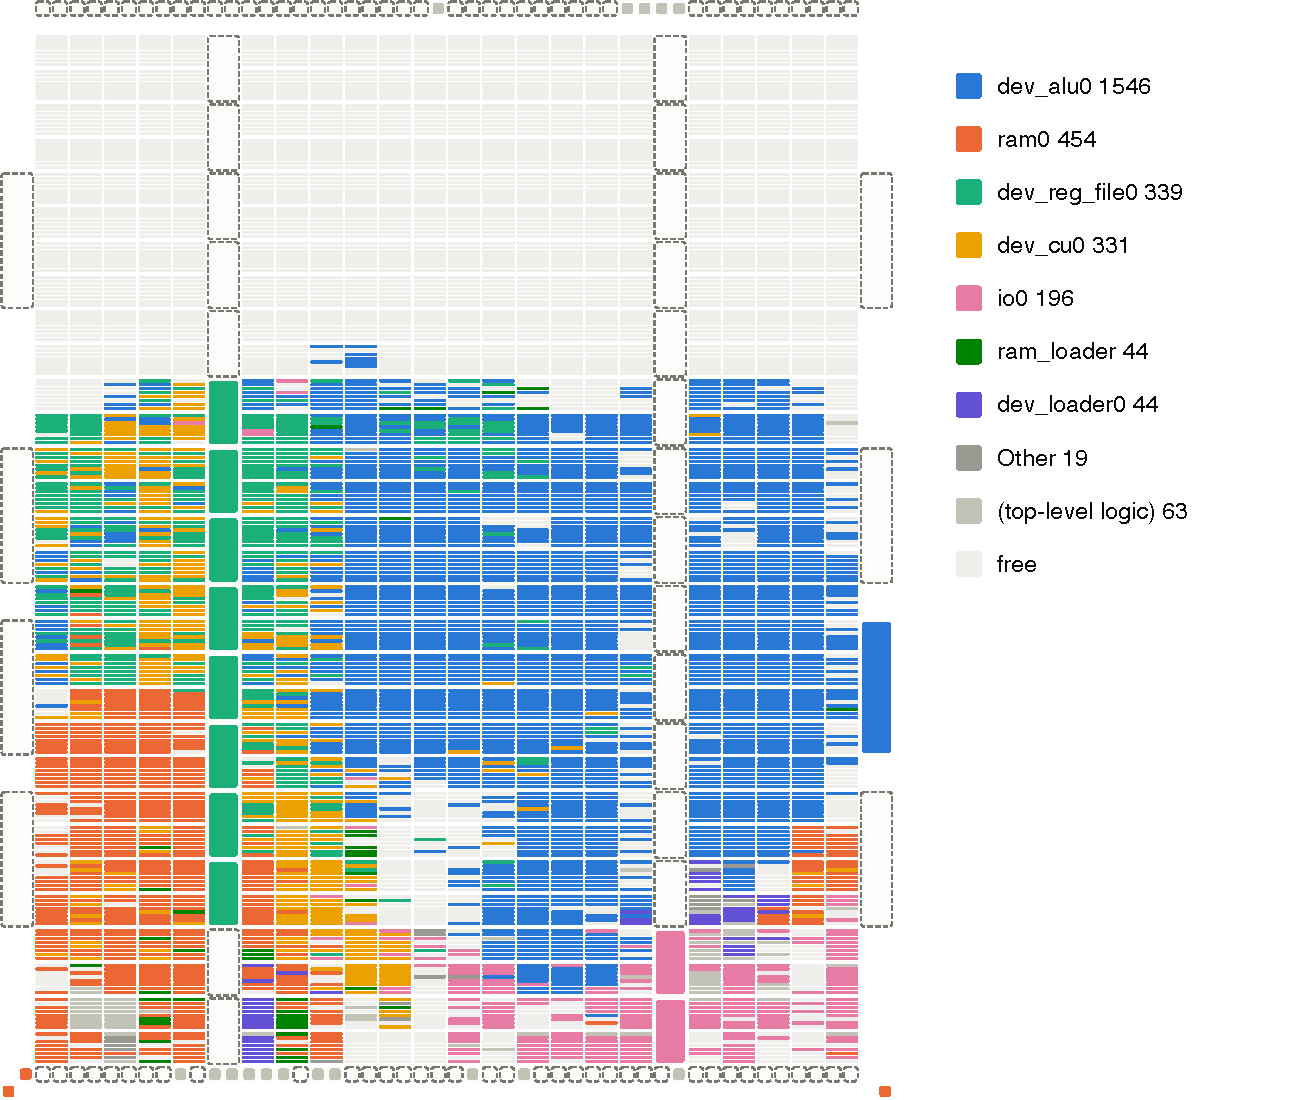
\includegraphics[width=0.85\linewidth]{figures/tools_floorplan.pdf}
\caption{The chip view of \cc{make floorplan} for step 09, with the number of
logic cells per top-level instance. The block RAMs of the register file
(\cc{dev_reg_file0}) form a column in the left half; the DSP used by the ALU
is the box on the right edge.}
\label{fig:tools-floorplan}
\end{figure}

\begin{pitfall}
The page knows only the names of the cells. yosys names a cell after the
net it drives, and after flattening this name begins with the instance path,
like \cc{dev_hex0.counter[3]} in Section~\ref{sec:step03-yosys}. The page
counts a cell for the instance at the beginning of its name. This is a good
approximation, but a cell at the boundary between two modules, for instance a
LUT that computes an input of one module from outputs of another, may be
named after the other module and be counted there. Cells whose names have no
instance path, and the extra cells nextpnr adds itself, appear as
``(top-level logic)''. So the numbers of the page and of \cc{make report}
differ a little.
\end{pitfall}

\section{make clean}

\cc{make clean} removes everything the Makefile creates: \cc{.stamp.*},
\cc{obj_dir}, \cc{waveform.vcd}, \cc{test.v}, the files of synthesis, place
and route and programming, the pictures, the report and the floorplan. The
sources (\cc{*.sv}, \cc{tb_test.cpp}) are never touched.

\chapter{Glossary}
\label{app:glossary}

The chapter in parentheses is where a term is introduced.

\begin{description}
\item[\cc{always_comb}] A block describing combinational logic: its outputs
  follow its inputs, without memory. Assignments with \cc{=}.
  (Chapter~\ref{ch:step01})
\item[\cc{always_ff}] A block describing flip-flops, here always written as
  \cc{always_ff @ (posedge clock)}: the signals assigned in it take their new
  values at the rising edge of the clock. Assignments with \cc{<=}.
  (Chapter~\ref{ch:step02})
\item[\cc{assign}] A permanent connection: the left side is a wire that always
  carries the value of the right side. (Chapter~\ref{ch:step01})
\item[Baud rate] The number of bits per second on a serial line.
  (Chapter~\ref{ch:step06})
\item[Attribute] A hint for the tools, attached to a declaration and
  written between \cc{(*} and \cc{*)}, for example \cc{(* no_rw_check *)}
  for a memory.
  (Chapter~\ref{ch:step07})
\item[Bitstream] The configuration of the FPGA as a bit pattern, written by
  icepack into \cc{test.bin}. (Chapter~\ref{ch:overview})
\item[Block RAM] One of the 30 memory blocks of 4\,kbit of the iCE40UP5K
  (\cc{SB_RAM40_4K}). yosys uses them for arrays that are read through a
  register. (Chapter~\ref{ch:step07})
\item[Bouncing] A mechanical button opens and closes several times within a
  few milliseconds before it settles. (Chapter~\ref{ch:step02})
\item[Carry chain] Dedicated wiring between neighbouring logic cells for the
  carry bits of an adder (\cc{SB_CARRY}). (Chapter~\ref{ch:step03})
\item[Clock domain] All flip-flops driven by the same clock.
  (Chapter~\ref{ch:step05})
\item[Clock enable] An input of a flip-flop that decides whether it takes
  over its data input at a clock edge (\cc{SB_DFFE}). A counter with an enable
  divides the clock without creating a new clock. (Chapter~\ref{ch:step03})
\item[Combinational logic] Logic without memory: its outputs are a function
  of its current inputs. (Chapter~\ref{ch:step01})
\item[Concatenation] \cc{\{a, b\}}: the bits of \cc{a} followed by those of
  \cc{b}, as one vector. (Chapter~\ref{ch:step03})
\item[Control unit] The part of the processor that fetches, decodes and
  executes instructions, as a state machine. (Chapter~\ref{ch:step09})
\item[Critical path] The slowest path between two flip-flops (or pins). Its
  delay determines the highest possible clock frequency.
  (Chapter~\ref{ch:step01})
\item[Debouncer] A circuit that accepts a new level of a button only after
  it has been stable for some milliseconds, and reports each press as a
  single-cycle pulse. (Chapters~\ref{ch:step05} and~\ref{ch:step07})
\item[Decoder] The combinational logic that turns the bits of an instruction
  into the control signals of the datapath. (Chapters~\ref{ch:step05}
  and~\ref{ch:step09})
\item[DSP block] A hard multiplier on the chip (\cc{SB_MAC16}); the
  iCE40UP5K has eight. (Chapter~\ref{ch:step09})
\item[FIFO] A first-in, first-out buffer: a memory with a write pointer and a
  read pointer, used as a ring. (Chapter~\ref{ch:step07})
\item[Flip-flop] A one-bit memory that takes over its input at the rising edge
  of its clock. Every logic cell has one. (Chapter~\ref{ch:step02})
\item[Fmax] The highest clock frequency at which the critical path still
  settles in time, as computed by nextpnr. (Chapter~\ref{ch:step02})
\item[FPGA] Field programmable gate array: a chip of configurable logic cells,
  routing, I/O pins and memory blocks. (Chapter~\ref{ch:overview})
\item[\cc{function}] A function in SystemVerilog. In our designs it computes
  constants while the tools process the design. (Chapter~\ref{ch:step06})
\item[Global network] One of eight wires that reach every flip-flop of the
  chip with little delay, used for clocks (\cc{SB_GB}).
  (Chapter~\ref{ch:step03})
\item[\cc{initial}] In our designs: the value a flip-flop has right after the
  FPGA is configured. (Chapter~\ref{ch:step02})
\item[Instantiation] Using a module inside another one, like a subcircuit in
  CircuitVerse. Each instance is its own copy of the hardware.
  (Chapter~\ref{ch:step03})
\item[\cc{interface}] A named bundle of wires, connected as a whole.
  (Chapter~\ref{ch:step07})
\item[Latch] A memory element that is transparent while its enable is
  active. yosys infers one when an \cc{always_comb} block does not assign a
  signal in every case, which is almost always a mistake.
  (Chapters~\ref{ch:step03} and~\ref{ch:step06})
\item[Logic cell] The basic building block of the FPGA: a LUT with four
  inputs, a flip-flop, and carry logic. The iCE40UP5K has 5280
  (\cc{ICESTORM_LC}). (Chapter~\ref{ch:overview})
\item[\cc{logic}] The type of a signal. Whether it becomes a wire or the
  output of a flip-flop follows from how it is assigned.
  (Chapter~\ref{ch:step01})
\item[LUT] Lookup table: a 16-to-1 multiplexer whose data inputs are
  configuration bits. It computes any Boolean function of four inputs.
  (Chapter~\ref{ch:overview})
\item[\cc{modport}] The view of an interface from one side: which of its wires
  are inputs and which are outputs there. (Chapter~\ref{ch:step07})
\item[Metastability] A flip-flop whose input changes right at the clock edge
  may hang between 0 and 1 for a while. (Chapter~\ref{ch:step04})
\item[Module] A circuit with ports, between \cc{module} and \cc{endmodule}.
  (Chapter~\ref{ch:step01})
\item[Netlist] A list of building blocks and of the wires between them, the
  result of synthesis (\cc{test.json}). (Chapter~\ref{ch:overview})
\item[Non-blocking assignment] \cc{<=} in \cc{always_ff}: all right-hand sides
  are taken from before the clock edge. (Chapter~\ref{ch:step02})
\item[Part-select] \cc{x[3:0]} or \cc{x[i +: 3]}: some bits of a vector.
  (Chapter~\ref{ch:step03})
\item[\cc{package}] A collection of constants and types, used with
  \cc{import} or \cc{pkg::name}. (Chapter~\ref{ch:step07})
\item[\cc{parameter}] A constant of a module that can be set differently for
  each instance. (Chapter~\ref{ch:step06})
\item[Pin file] \cc{icebreaker.pcf}: the names of the pins of the chip that a
  top module may use as ports. (Chapter~\ref{ch:overview})
\item[Place and route] Choosing a physical block for every building block of
  the netlist and switches for the wires between them; done by nextpnr.
  (Chapter~\ref{ch:overview})
\item[PMOD] A simple connector standard for small extension modules.
  (Chapter~\ref{ch:overview})
\item[Reduction] \cc{&x}, \cc{|x}, \cc{^x}: the AND, OR or XOR of all bits
  of a vector. (Chapter~\ref{ch:step07})
\item[Register file] The registers of a processor, with ports to read and to
  write them. (Chapters~\ref{ch:step05} and~\ref{ch:step09})
\item[Replication] \cc{\{n\{a\}\}}: \cc{a} repeated $n$ times, $n$ wires
  connected to the same signal. (Chapter~\ref{ch:step05})
\item[Seven-segment display] Seven LEDs arranged as an 8. Our display has two
  digits that share the segment wires and are switched on in turn
  (multiplexing). (Chapter~\ref{ch:step03})
\item[Simulation] Computing how all signals of a design change over time, here
  with Verilator and a testbench. (Chapter~\ref{ch:step01})
\item[Sized literal] A constant with a given number of bits, such as
  \cc{8'h0f} or \cc{1'b1}. (Chapter~\ref{ch:step03})
\item[SPRAM] One of the four single-port memory blocks of 256\,kbit of the
  iCE40UP5K (\cc{SB_SPRAM256KA}), together 128\,KiB.
  (Chapter~\ref{ch:step08})
\item[State machine] A register holding a state, and combinational logic
  computing the next state. (Chapters~\ref{ch:step02} and~\ref{ch:step06})
\item[Synchroniser] Flip-flops that bring an asynchronous input, such as a
  button or the serial line, into the clock domain of the design.
  (Chapters~\ref{ch:step04} and~\ref{ch:step06})
\item[Synthesis] Turning a description into a netlist of the building blocks
  of the FPGA; done by yosys. (Chapter~\ref{ch:overview})
\item[Testbench] A program that sets the inputs of a simulated design and
  records its signals. (Chapter~\ref{ch:step01})
\item[Top module] The outermost module of a design. Its ports are pins of the
  chip. (Chapter~\ref{ch:step01})
\item[\cc{typedef enum}] A type whose values have names, used for the states
  of state machines. (Chapter~\ref{ch:step06})
\item[UART] The circuit for a serial line: a start bit, eight data bits (least
  significant first), a stop bit. (Chapter~\ref{ch:step06})
\item[Vector] A signal of several bits, such as \cc{logic [7:0] x}.
  (Chapter~\ref{ch:step03})
\item[Waveform] The values of signals over time, as recorded in
  \cc{waveform.vcd} and shown by Surfer or GTKWave. (Chapter~\ref{ch:step01})
\end{description}

\end{document}
